\documentclass{article}
\usepackage{amsmath,mathtools}
\usepackage[utf8]{inputenc}
\usepackage[ngerman]{babel}
\usepackage{acronym}
\usepackage{graphicx} 
\usepackage{epstopdf}
\usepackage{svg}
\usepackage{multirow}

%Hyperlinks package, links aus inhaltsverzeichnis
\usepackage[hidelinks]{hyperref}
\hypersetup{
    colorlinks=false, %set true if you want colored links
    linktoc=all
}
%Blattformatierung
\usepackage{geometry}
\geometry{a4paper, top=25mm, left=30mm, right=25mm, bottom=20mm}

\begin{document}
\tableofcontents

\newpage
\section{Dynamische Störungen}
\subsection{Messplots $y_{11}=-tan(\varphi)$}
\subsubsection{Verlauf von $\varphi$ bei $T_M = sin(2\pi\cdot f \cdot t)$}
\begin{figure}[!h]
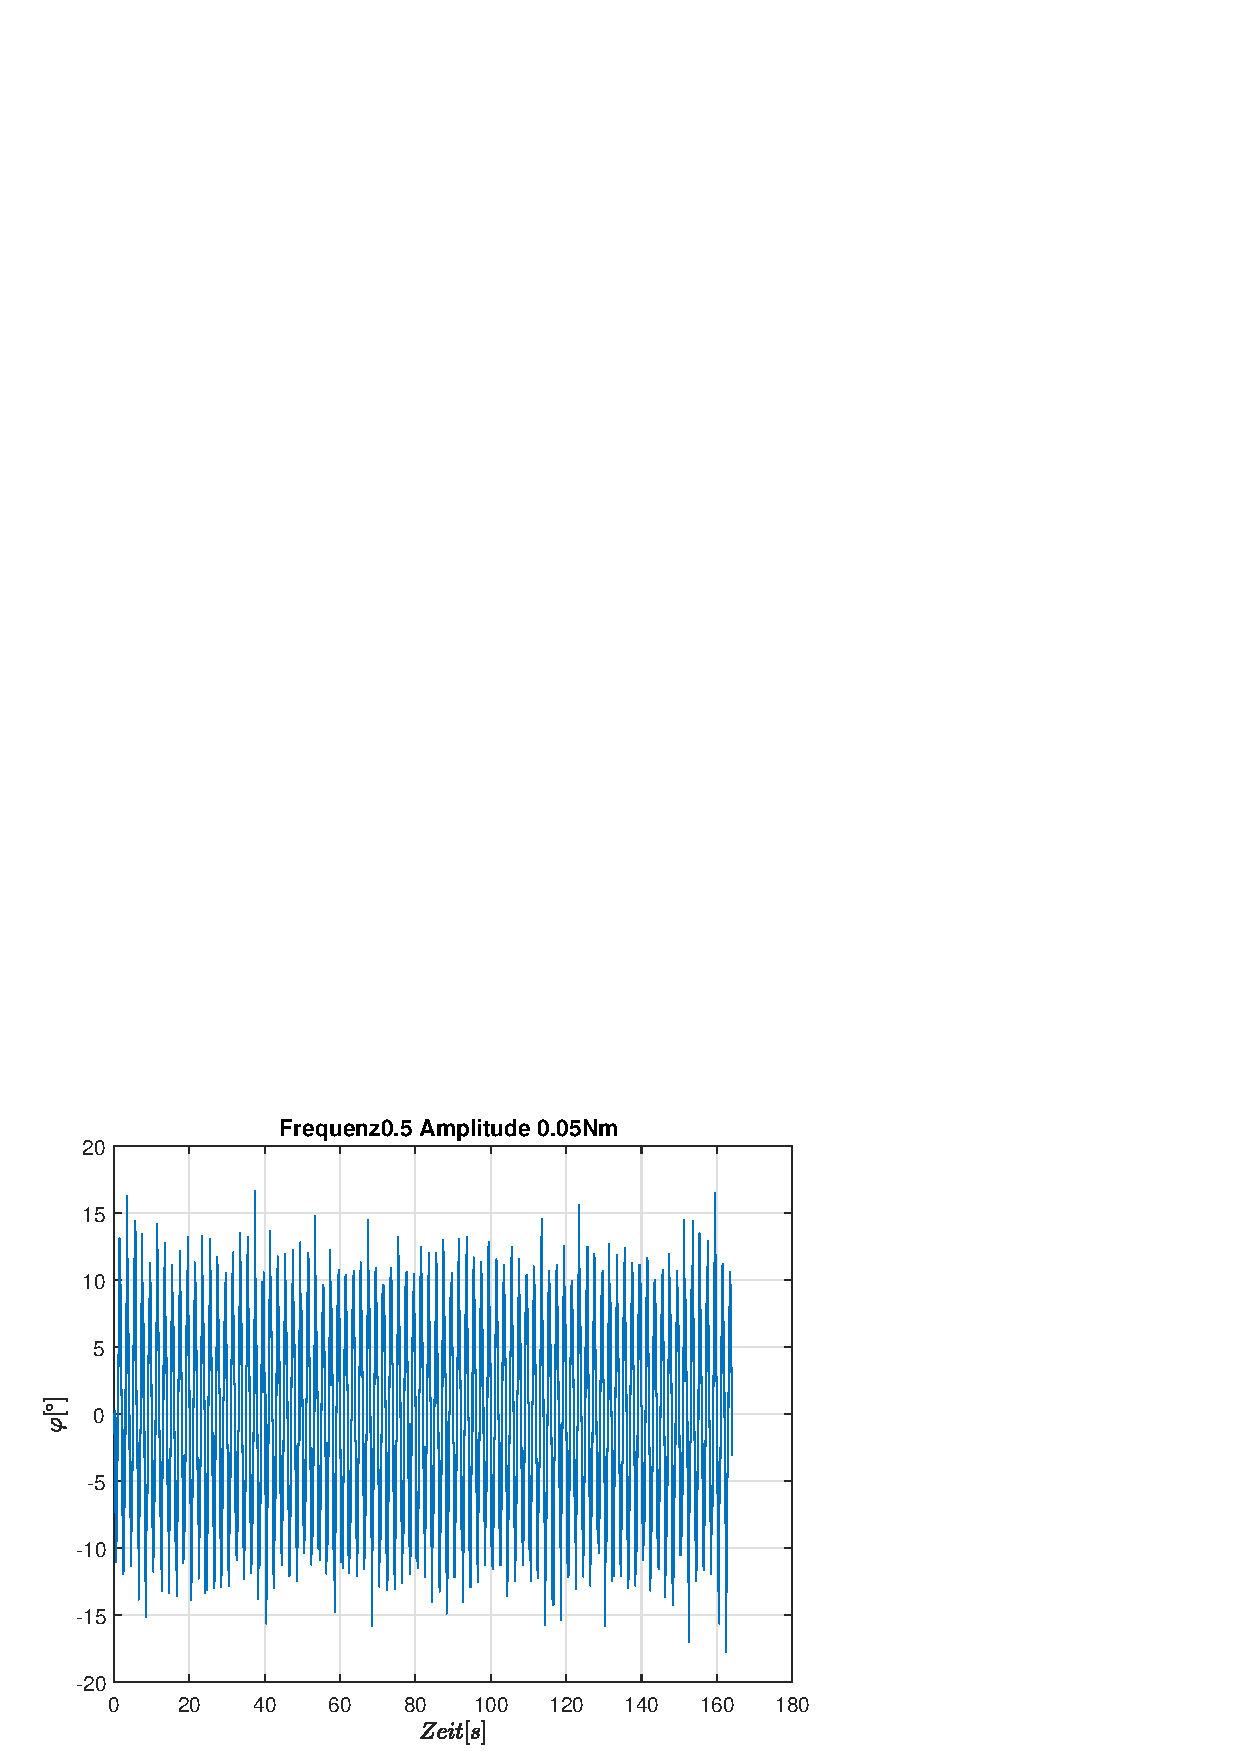
\includegraphics[width=0.5\linewidth]{img/phi_sinefreq_0_5}
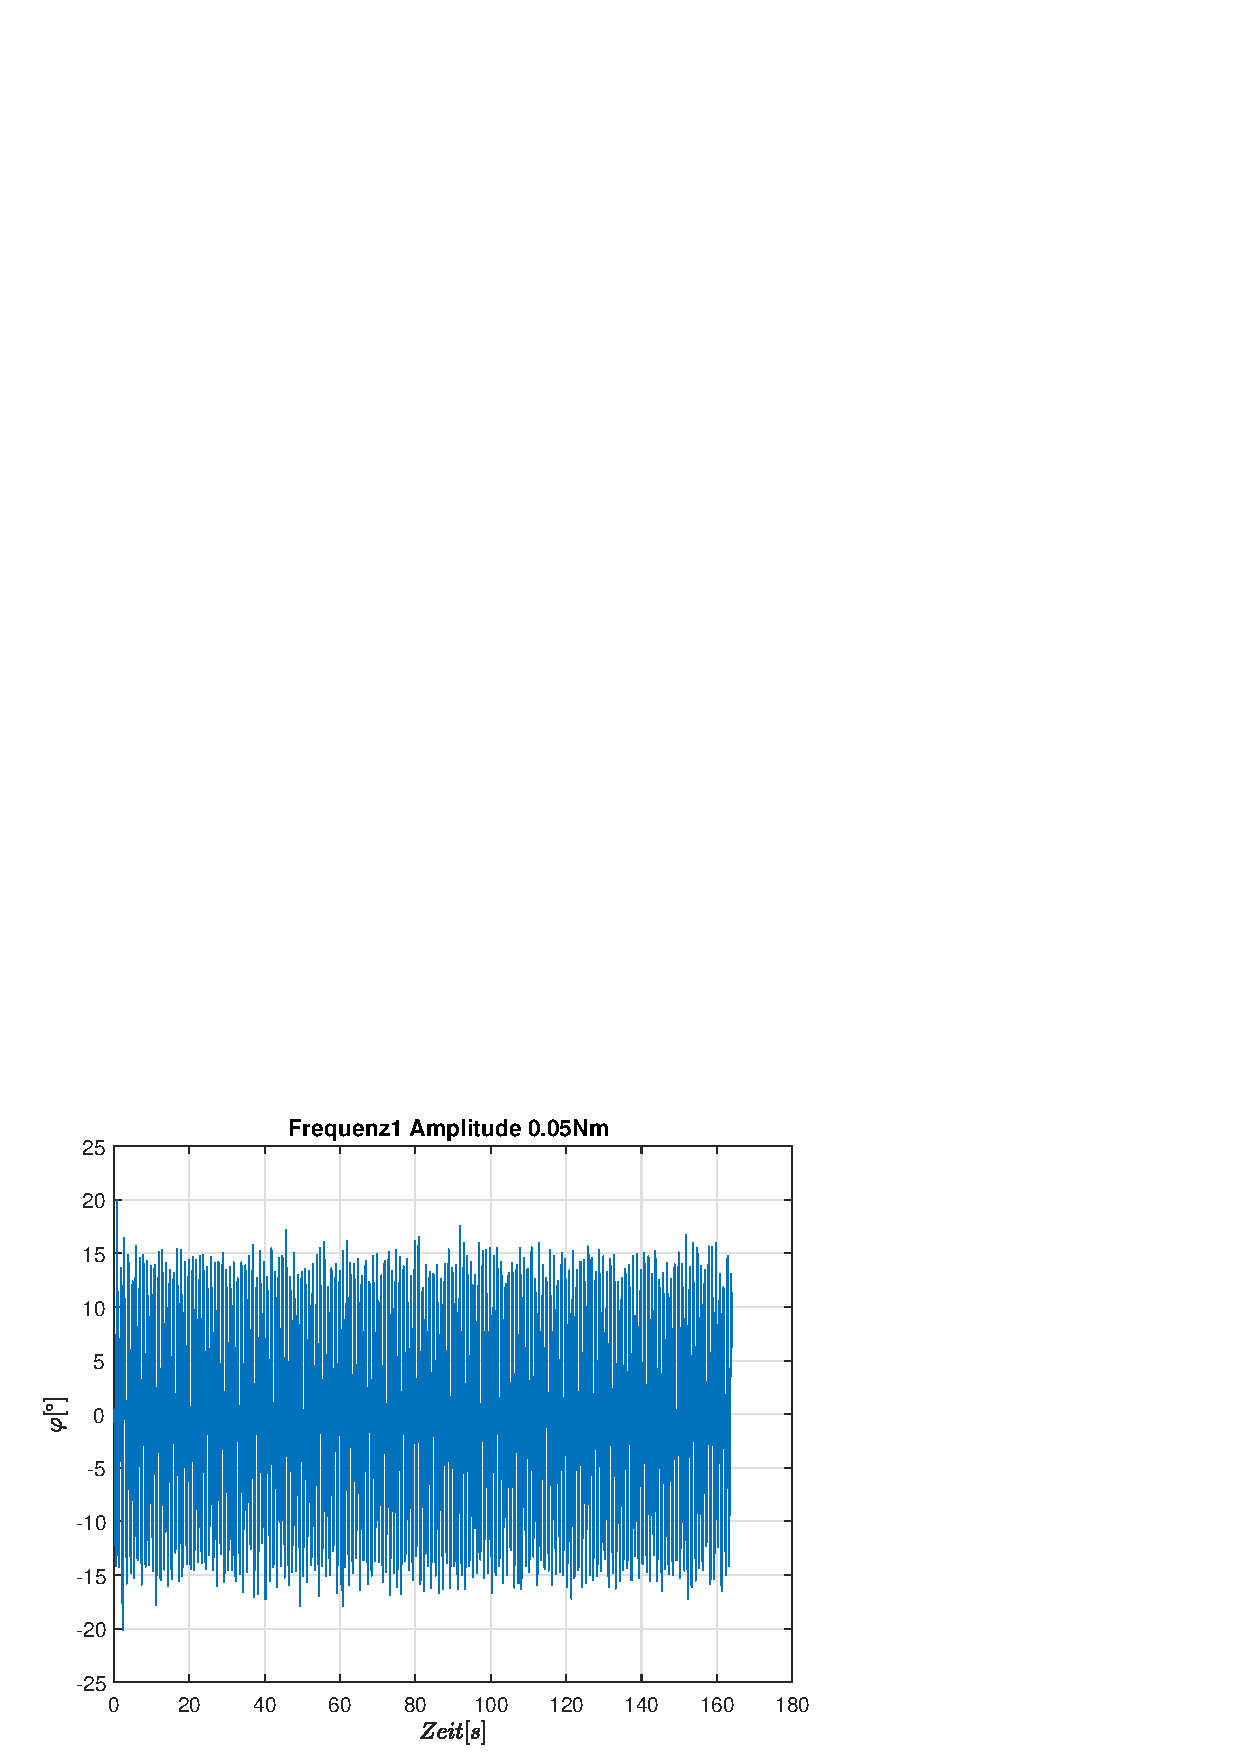
\includegraphics[width=0.5\linewidth]{img/phi_sinefreq_1}
\end{figure}
\begin{figure}[!h]
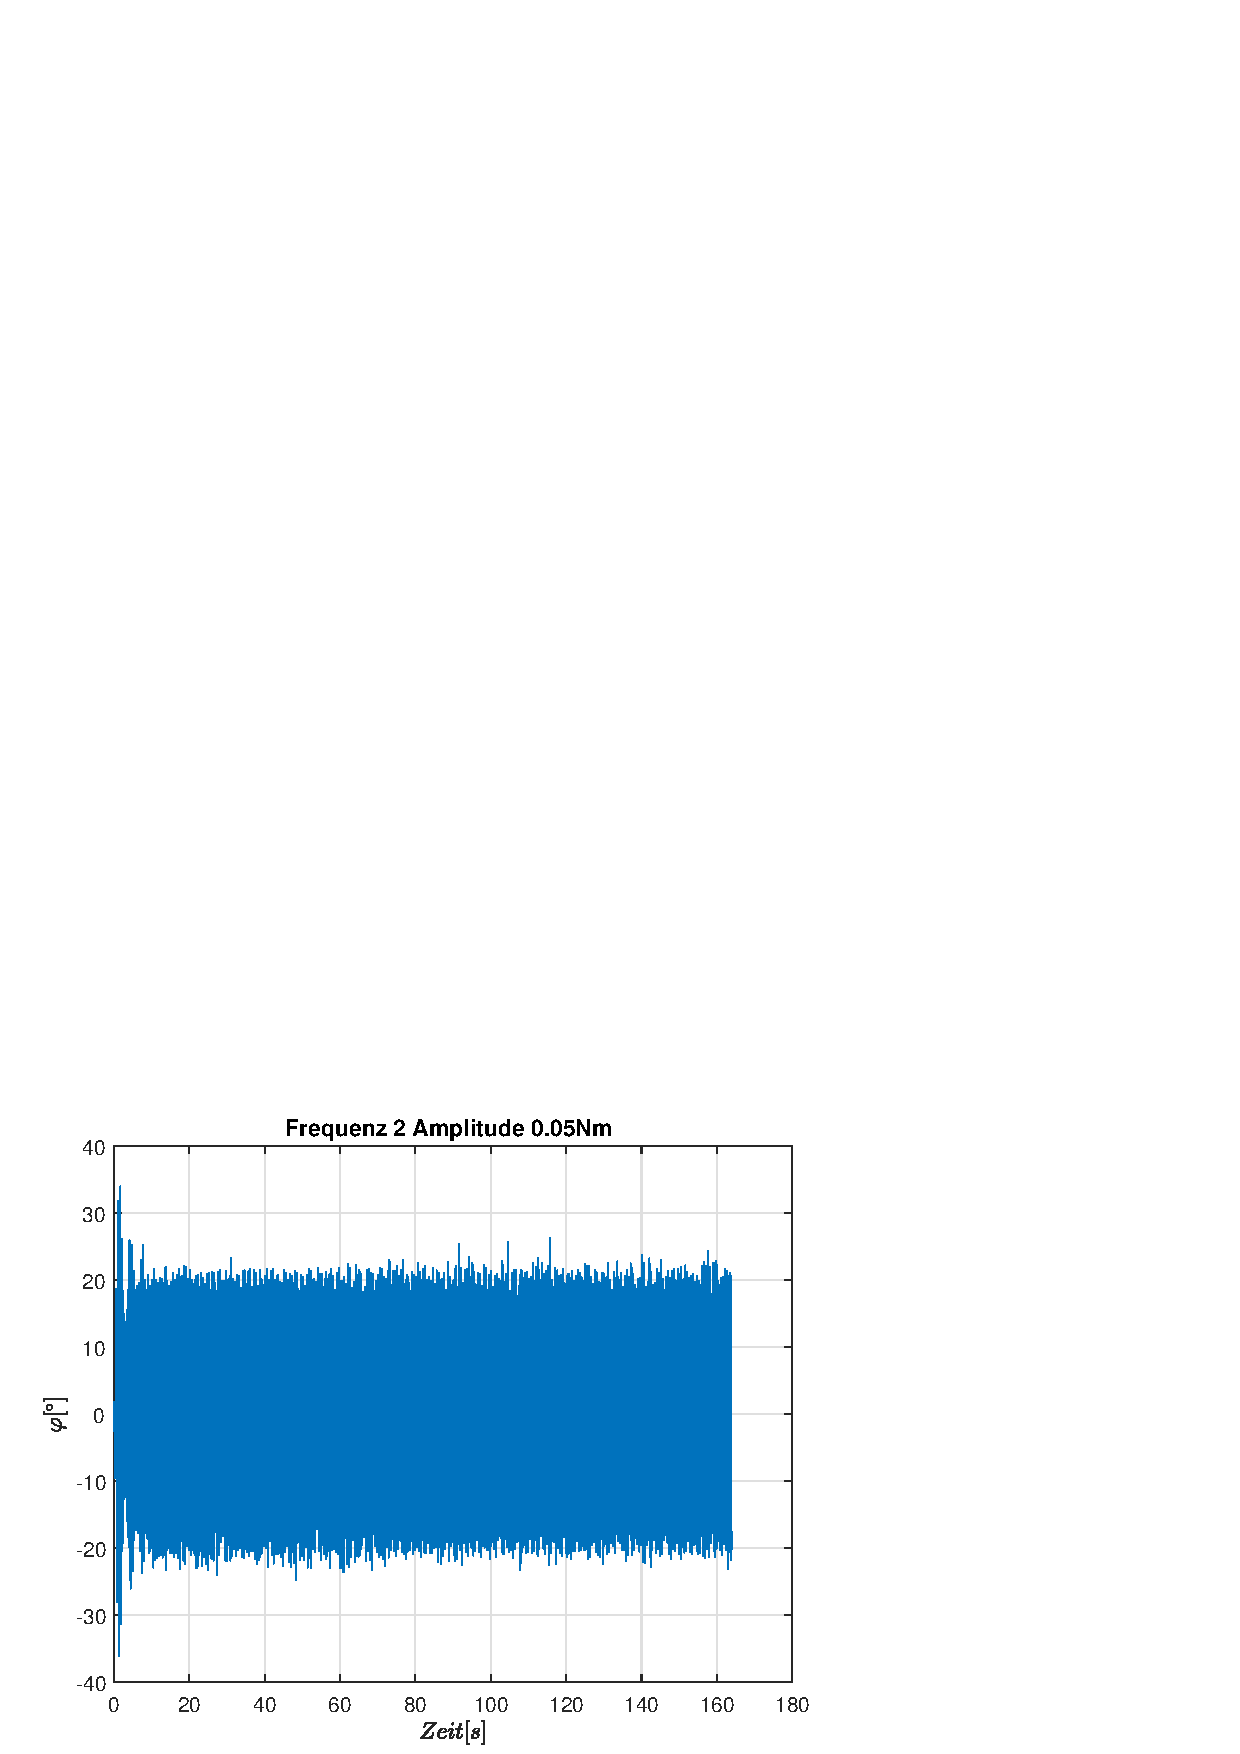
\includegraphics[width=0.5\linewidth]{img/phi_sinefreq_2}
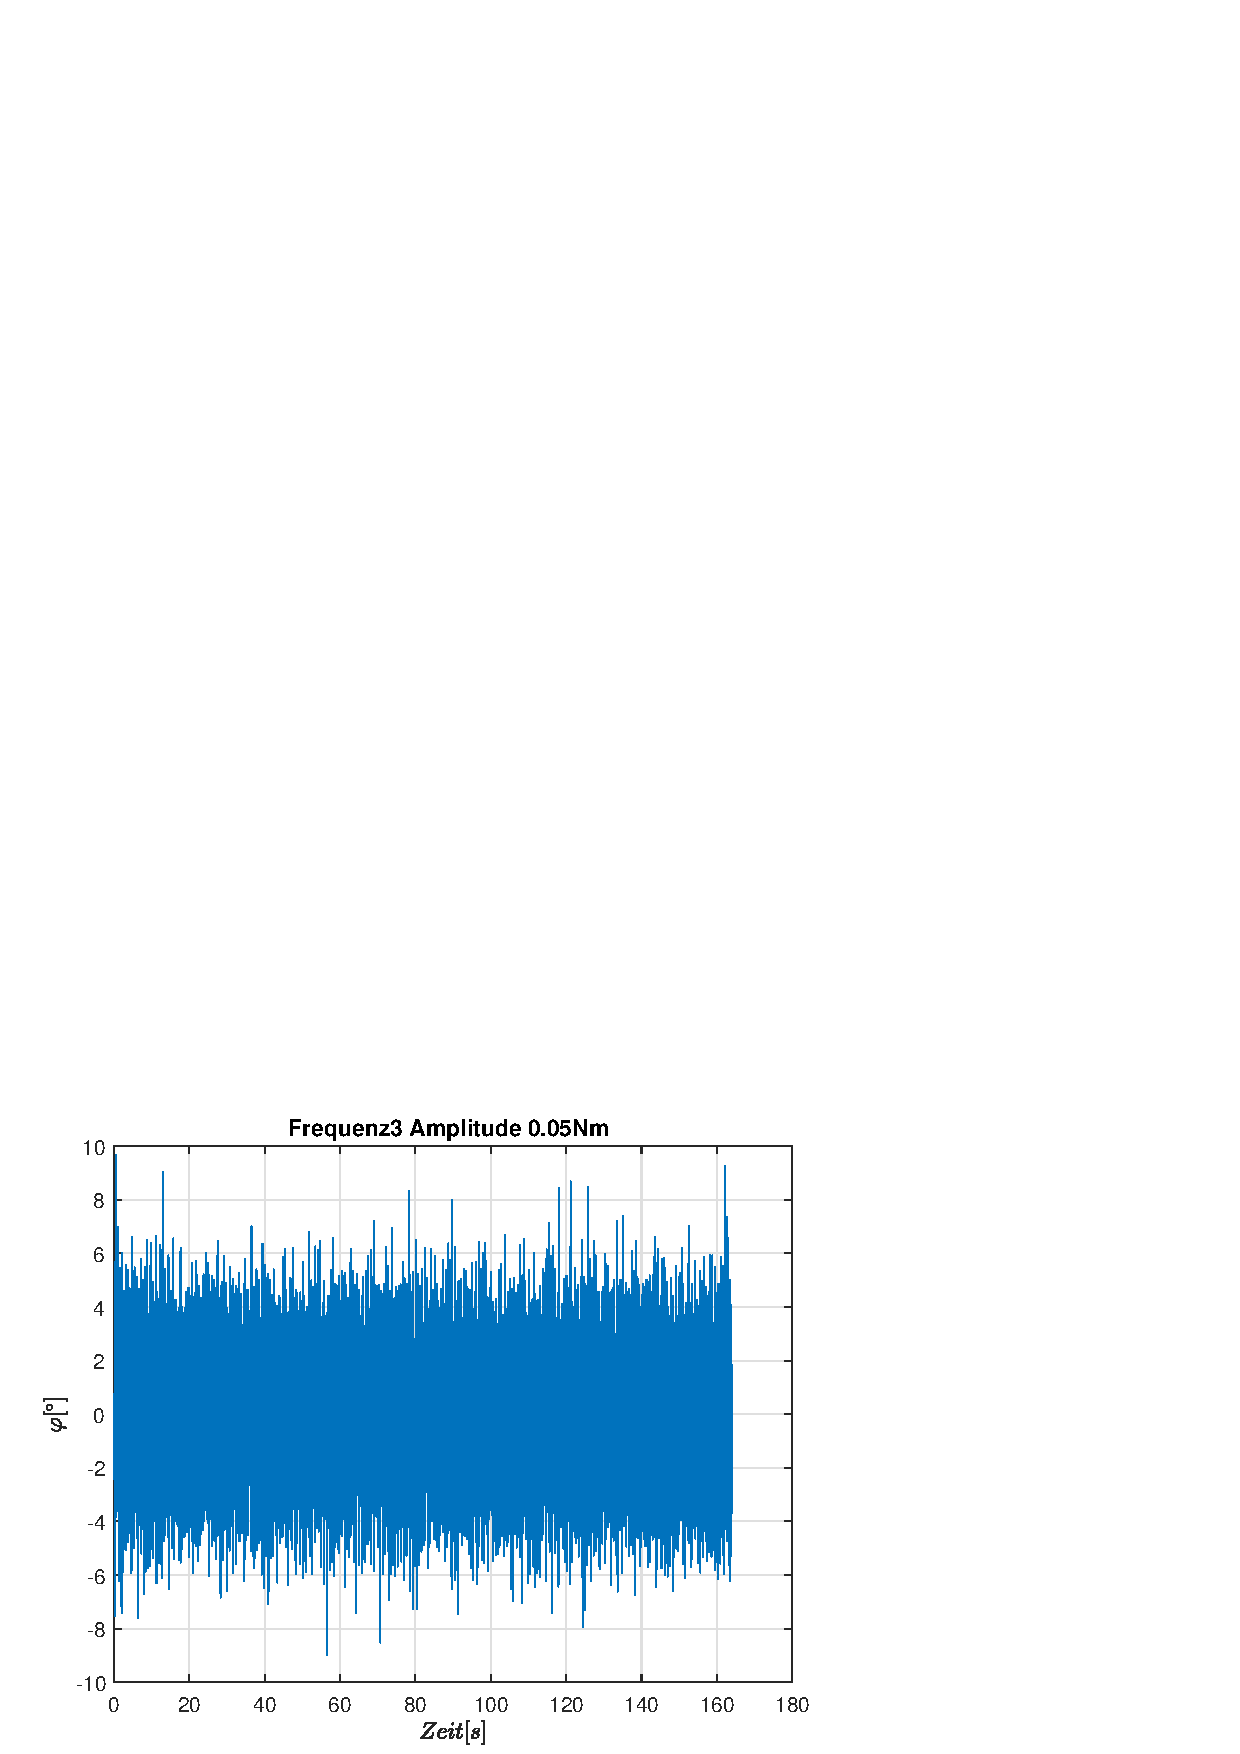
\includegraphics[width=0.5\linewidth]{img/phi_sinefreq_3}
\end{figure}
\begin{figure}[!h]
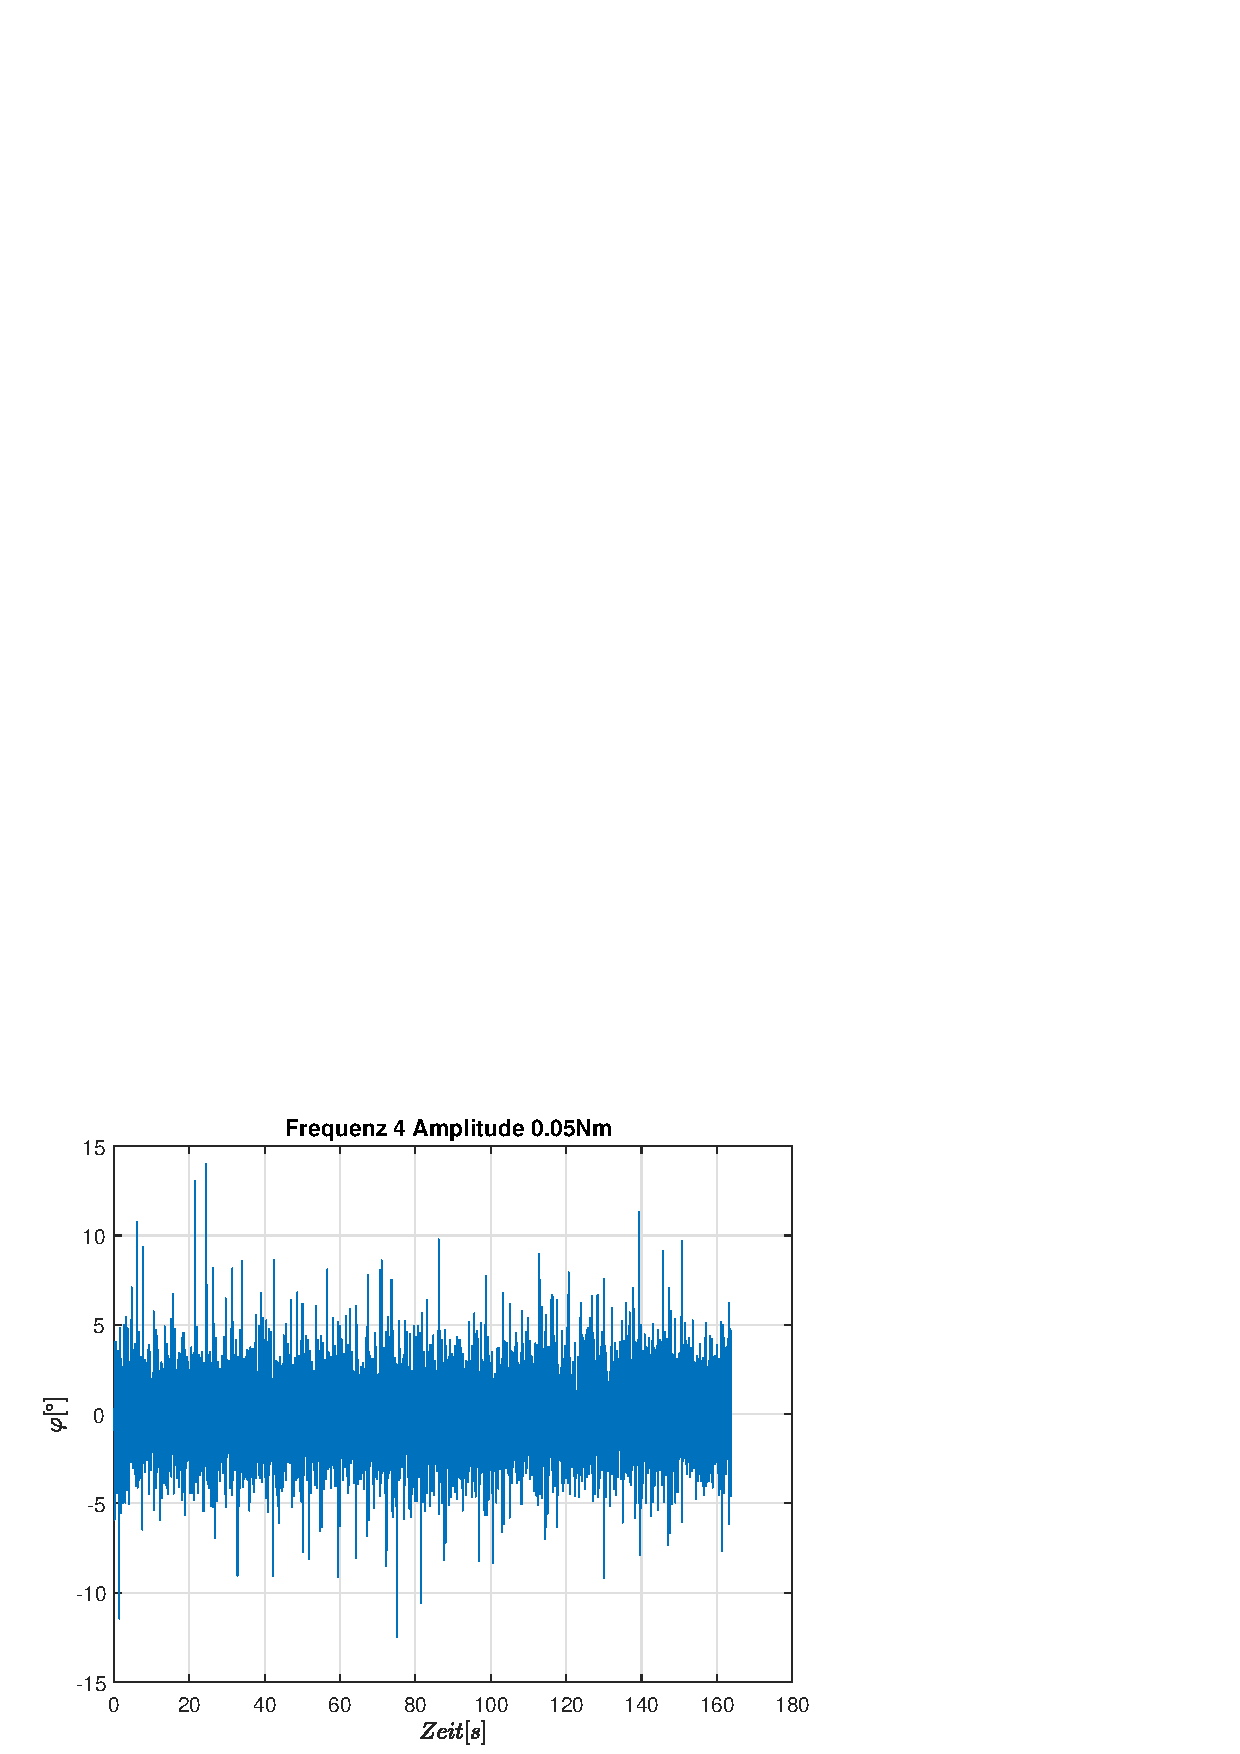
\includegraphics[width=0.5\linewidth]{img/phi_sinefreq_4}
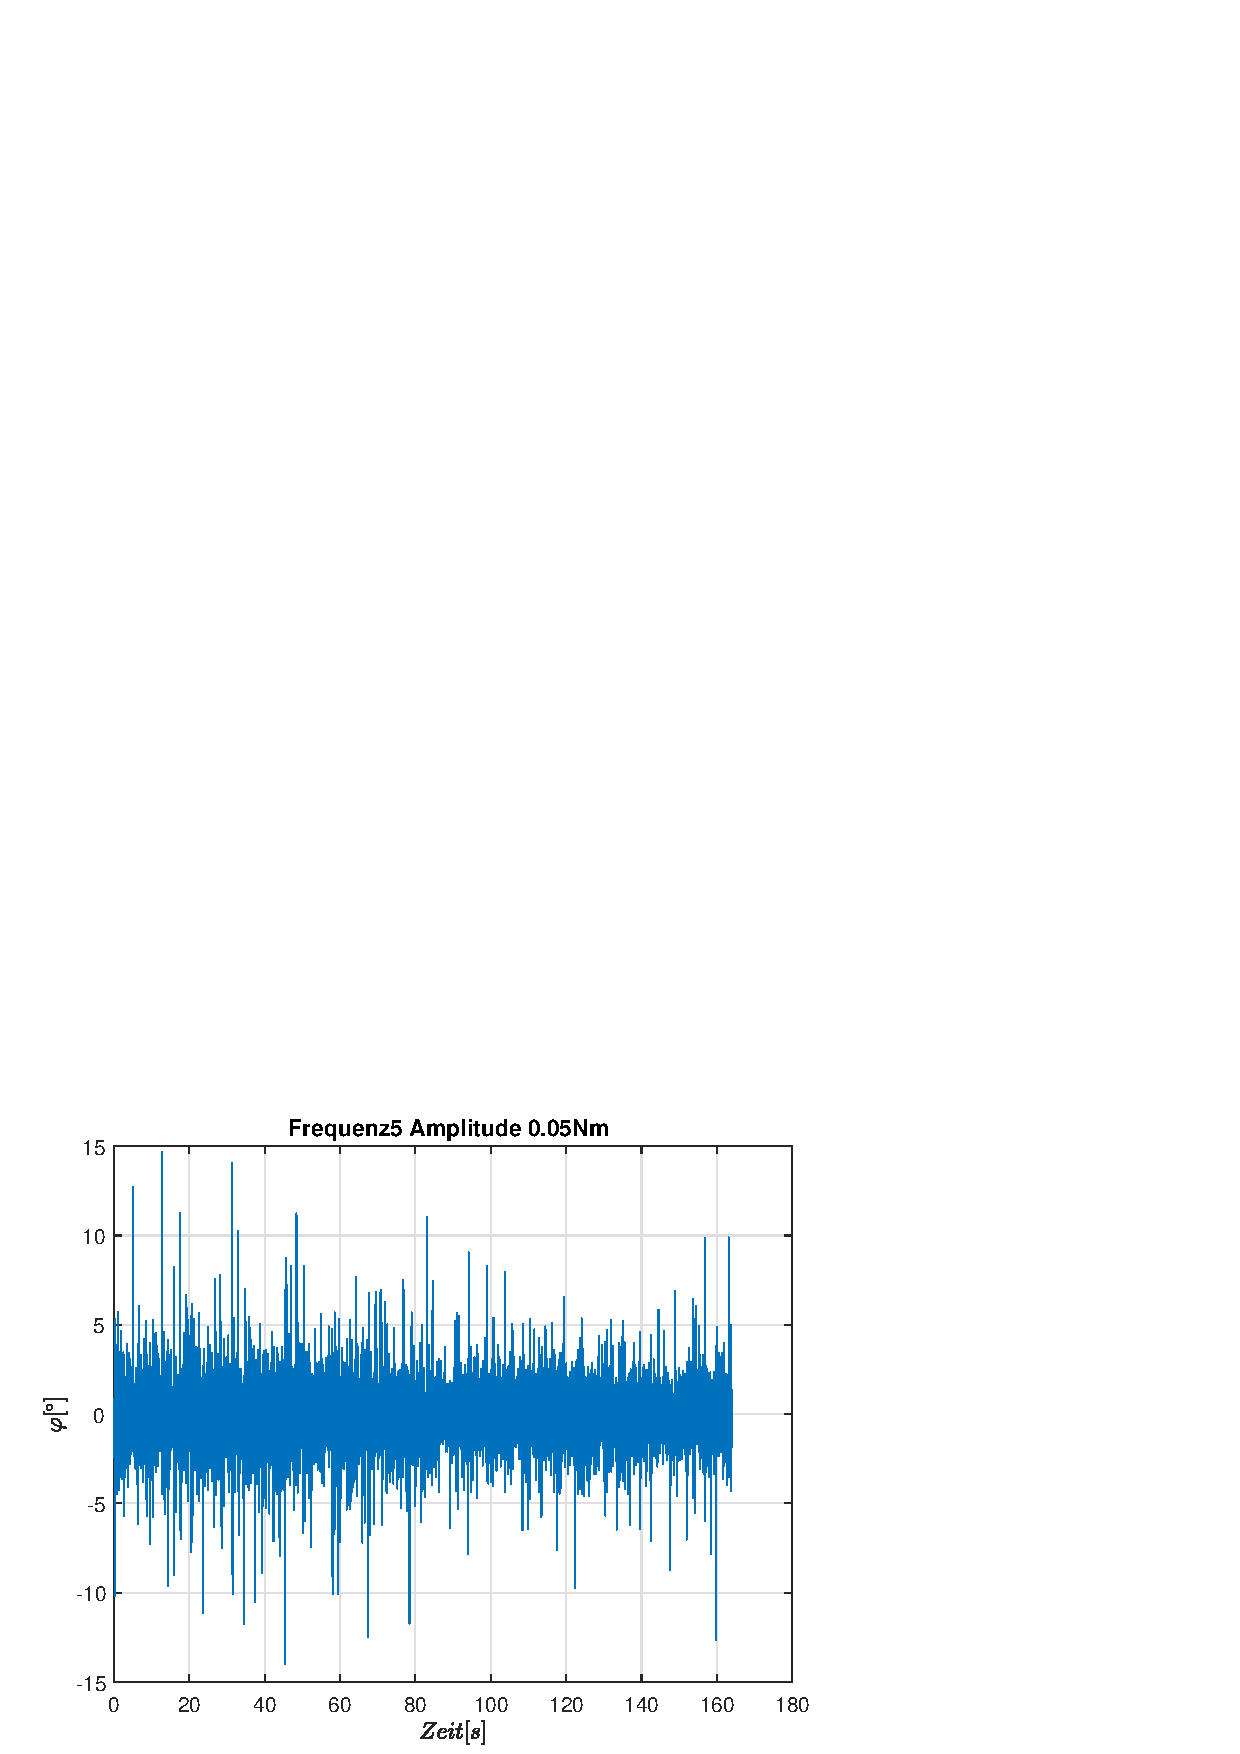
\includegraphics[width=0.5\linewidth]{img/phi_sinefreq_5}
\end{figure}
\begin{figure}[!h]
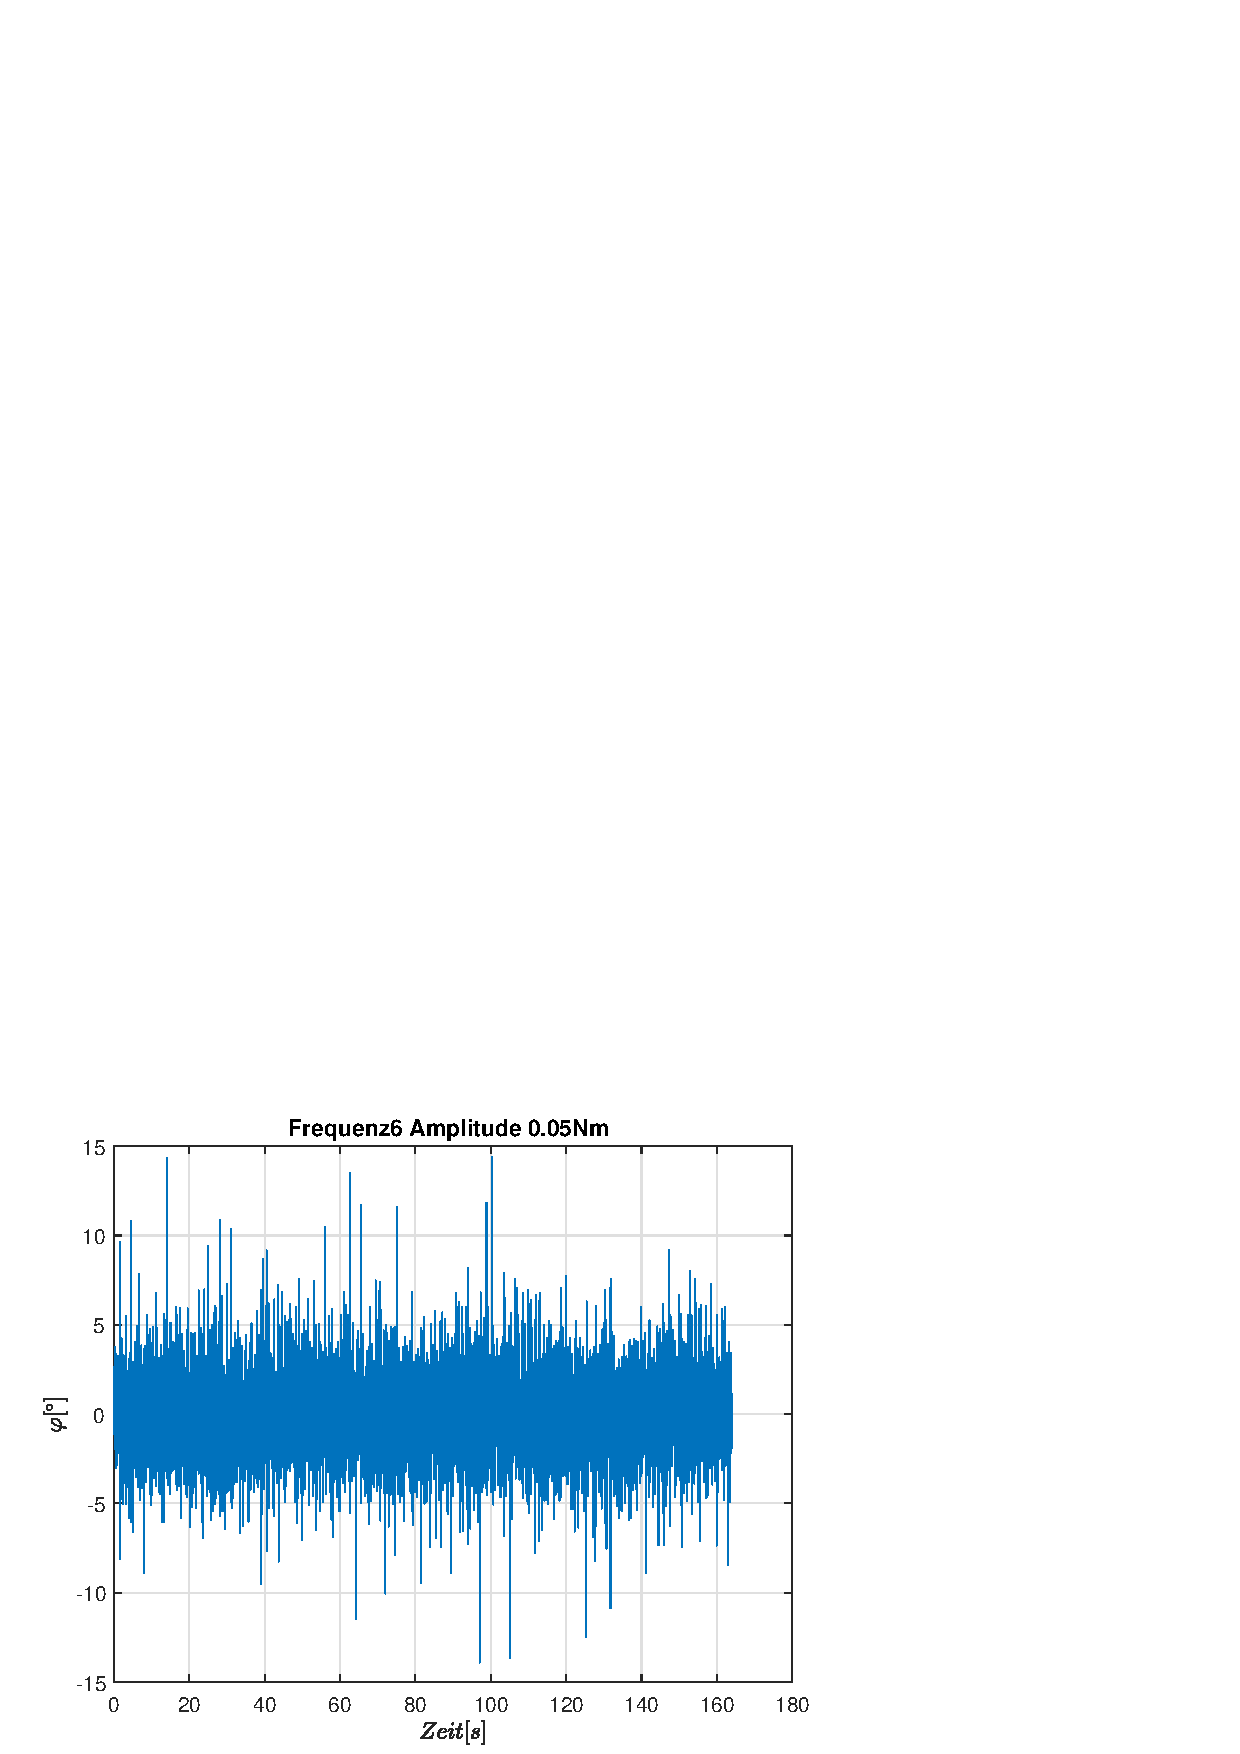
\includegraphics[width=0.5\linewidth]{img/phi_sinefreq_6}
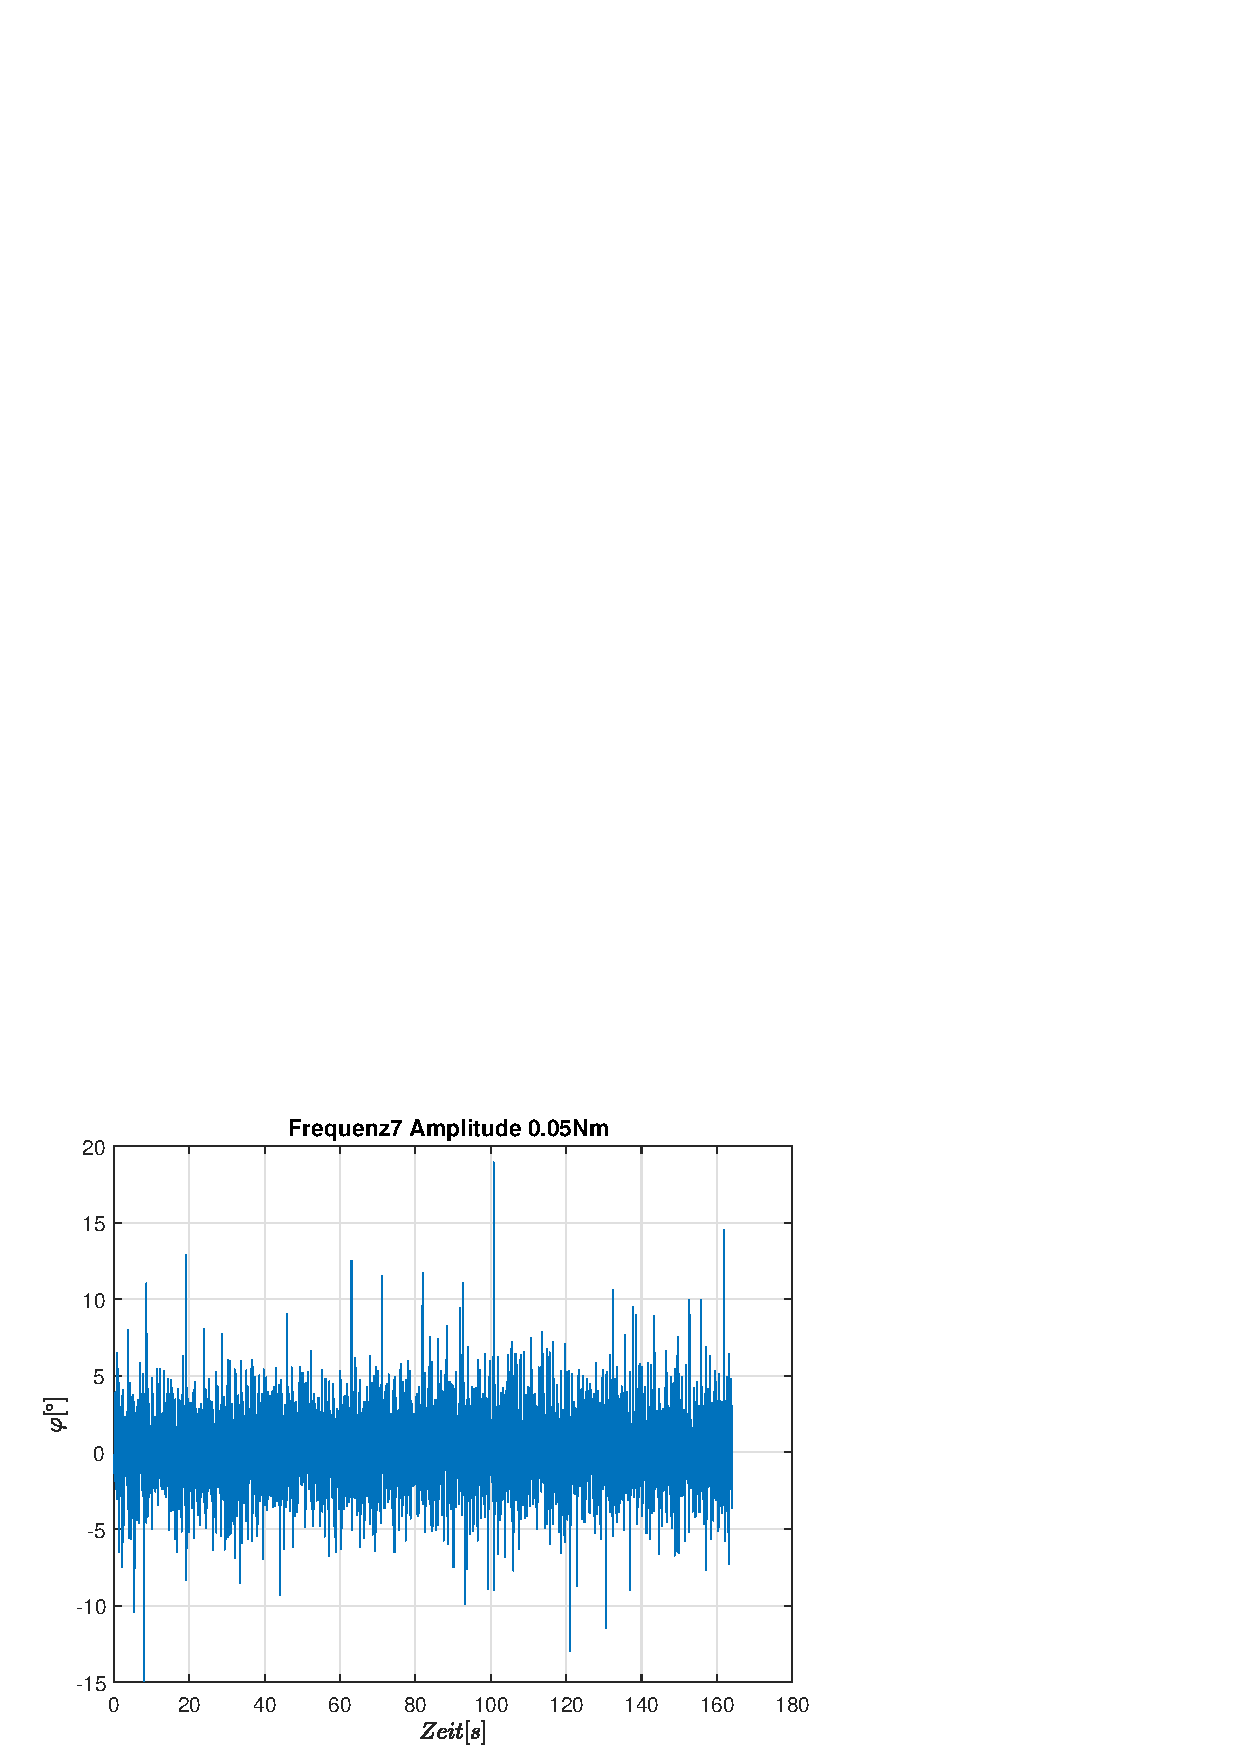
\includegraphics[width=0.5\linewidth]{img/phi_sinefreq_7}
\end{figure}
\begin{figure}[!h]
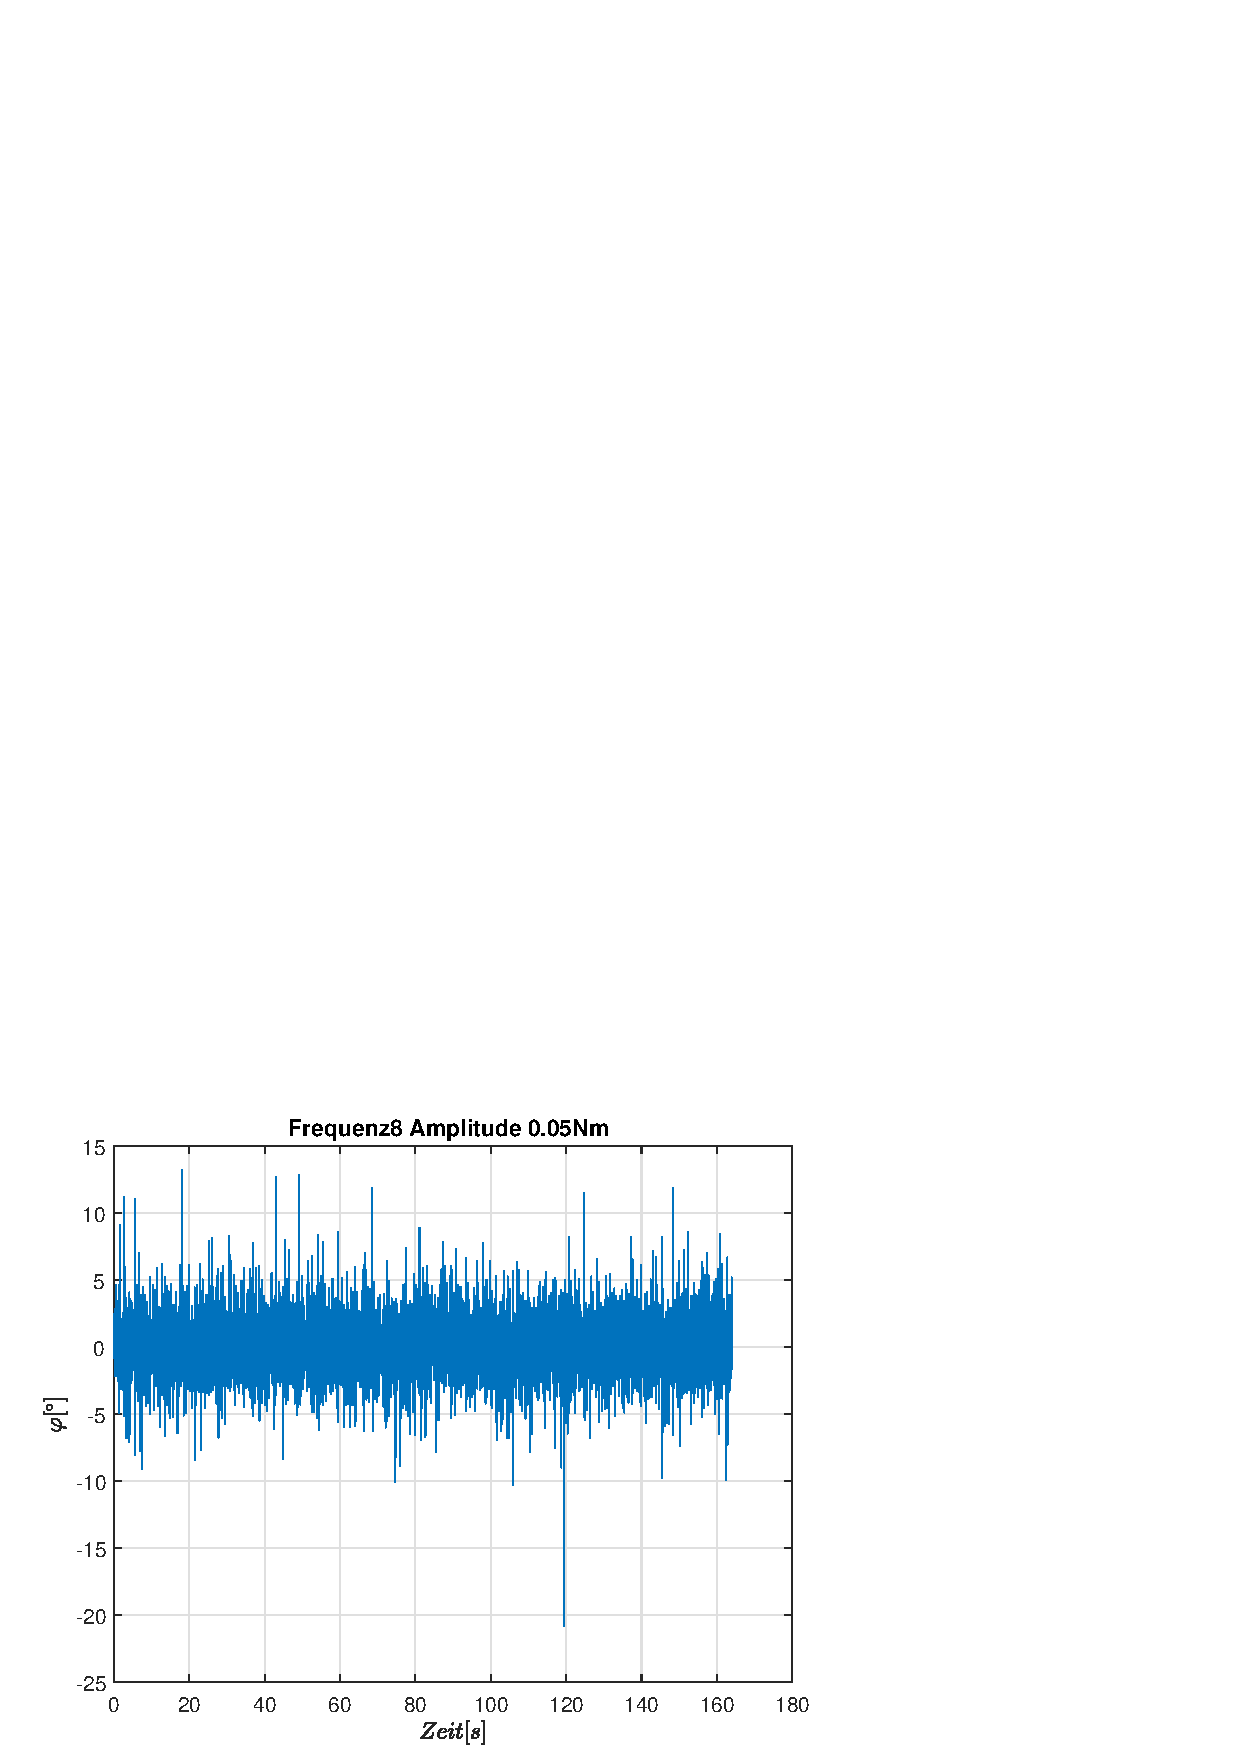
\includegraphics[width=0.5\linewidth]{img/phi_sinefreq_8}
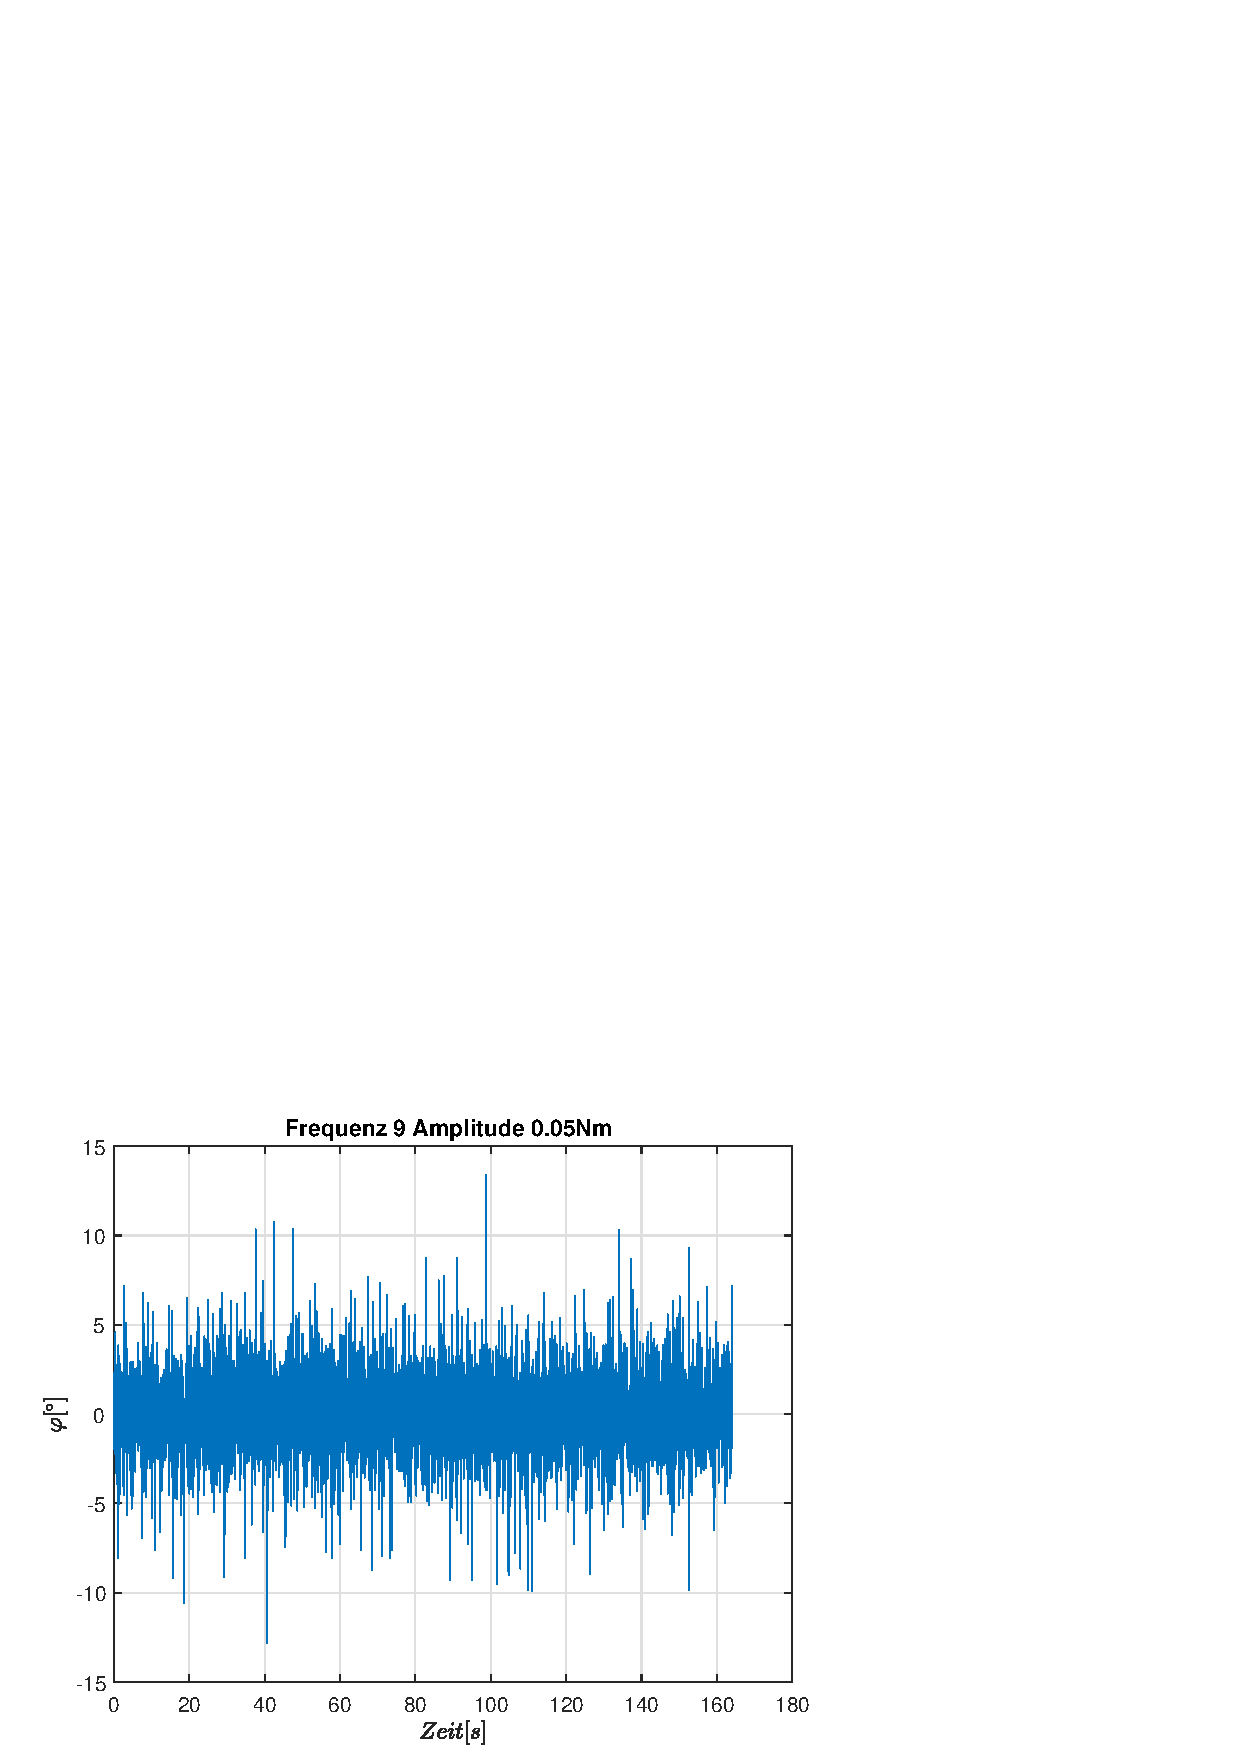
\includegraphics[width=0.5\linewidth]{img/phi_sinefreq_9}
\end{figure}
\begin{figure}[!h]
\centering
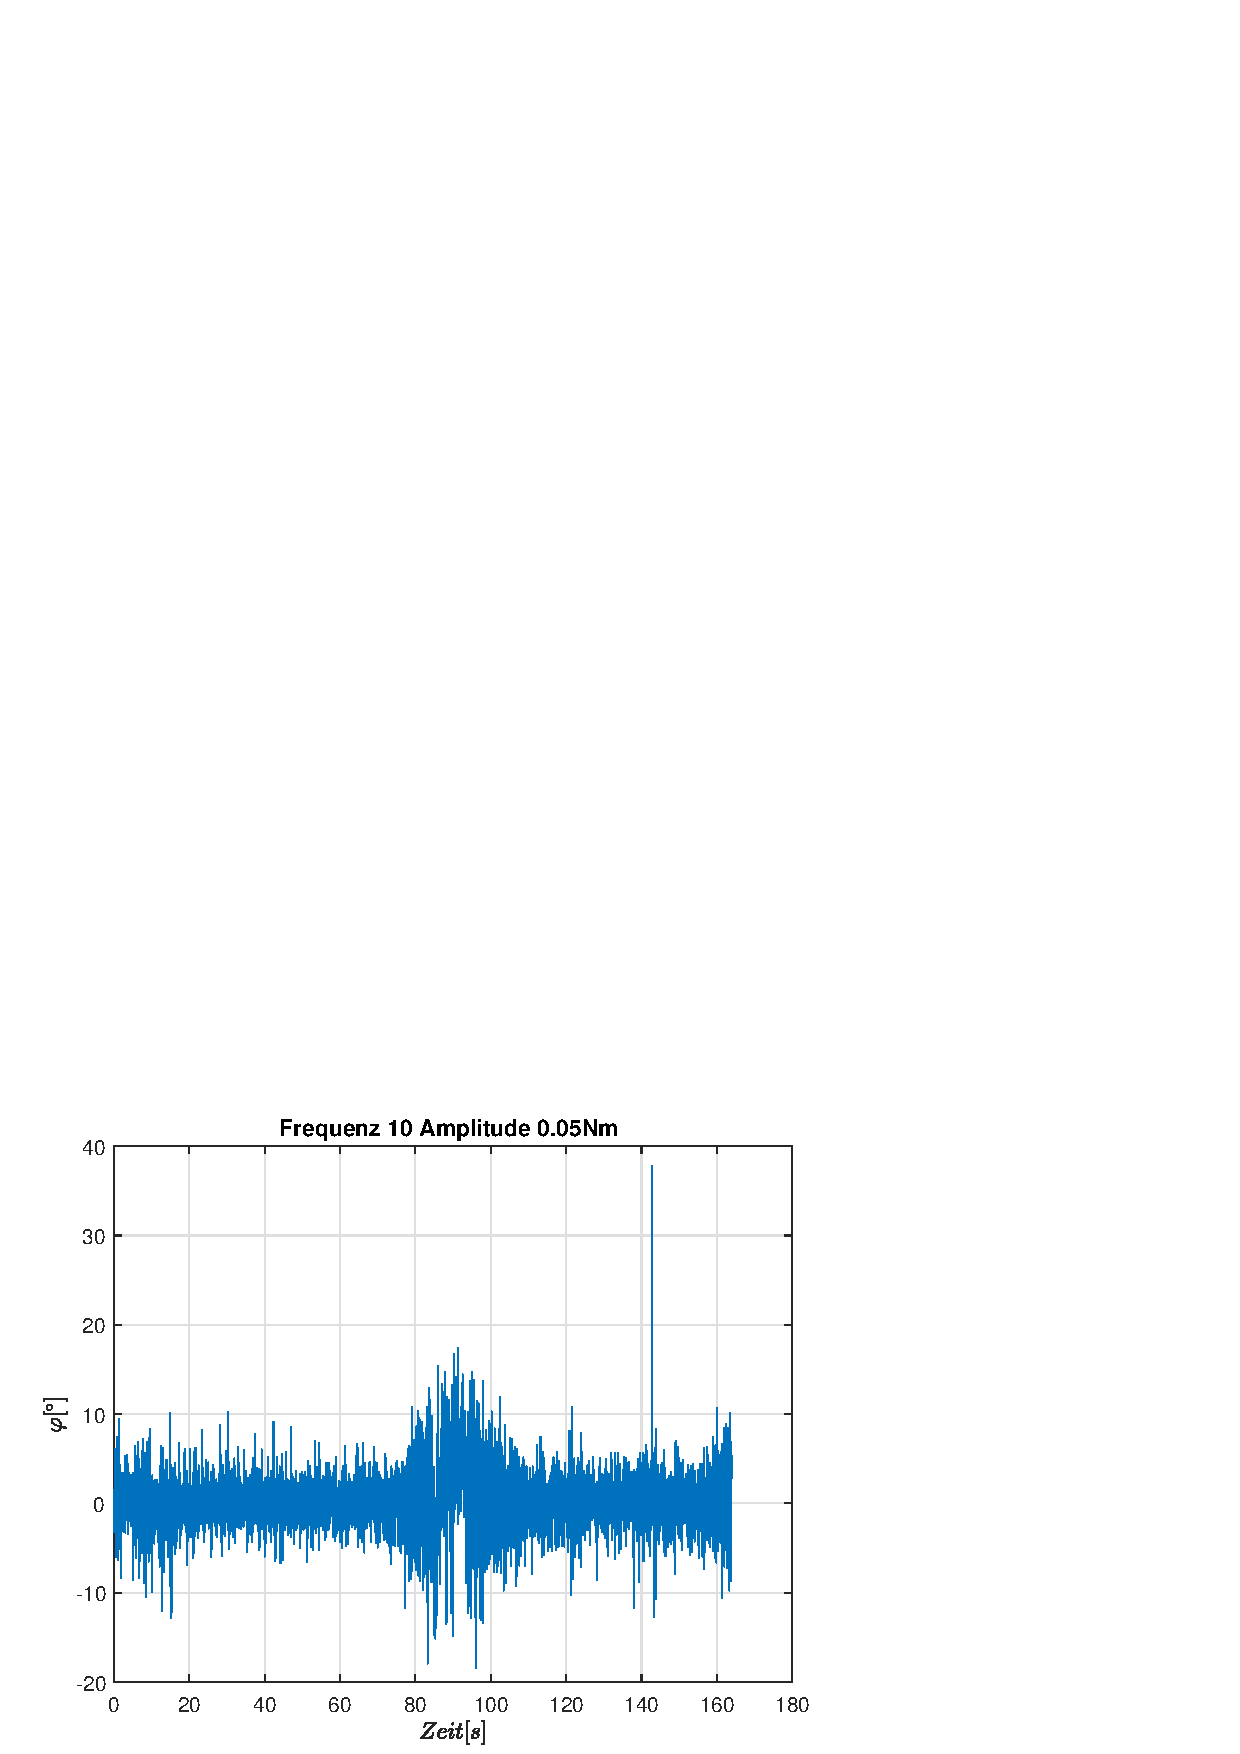
\includegraphics[width=0.5\linewidth]{img/phi_sinefreq_10}
\end{figure}

\newpage
\subsubsection{DFT-Spektren von $\varphi$ bei $T_M = sin(2\pi\cdot f \cdot t)$}
\begin{figure}[!h]
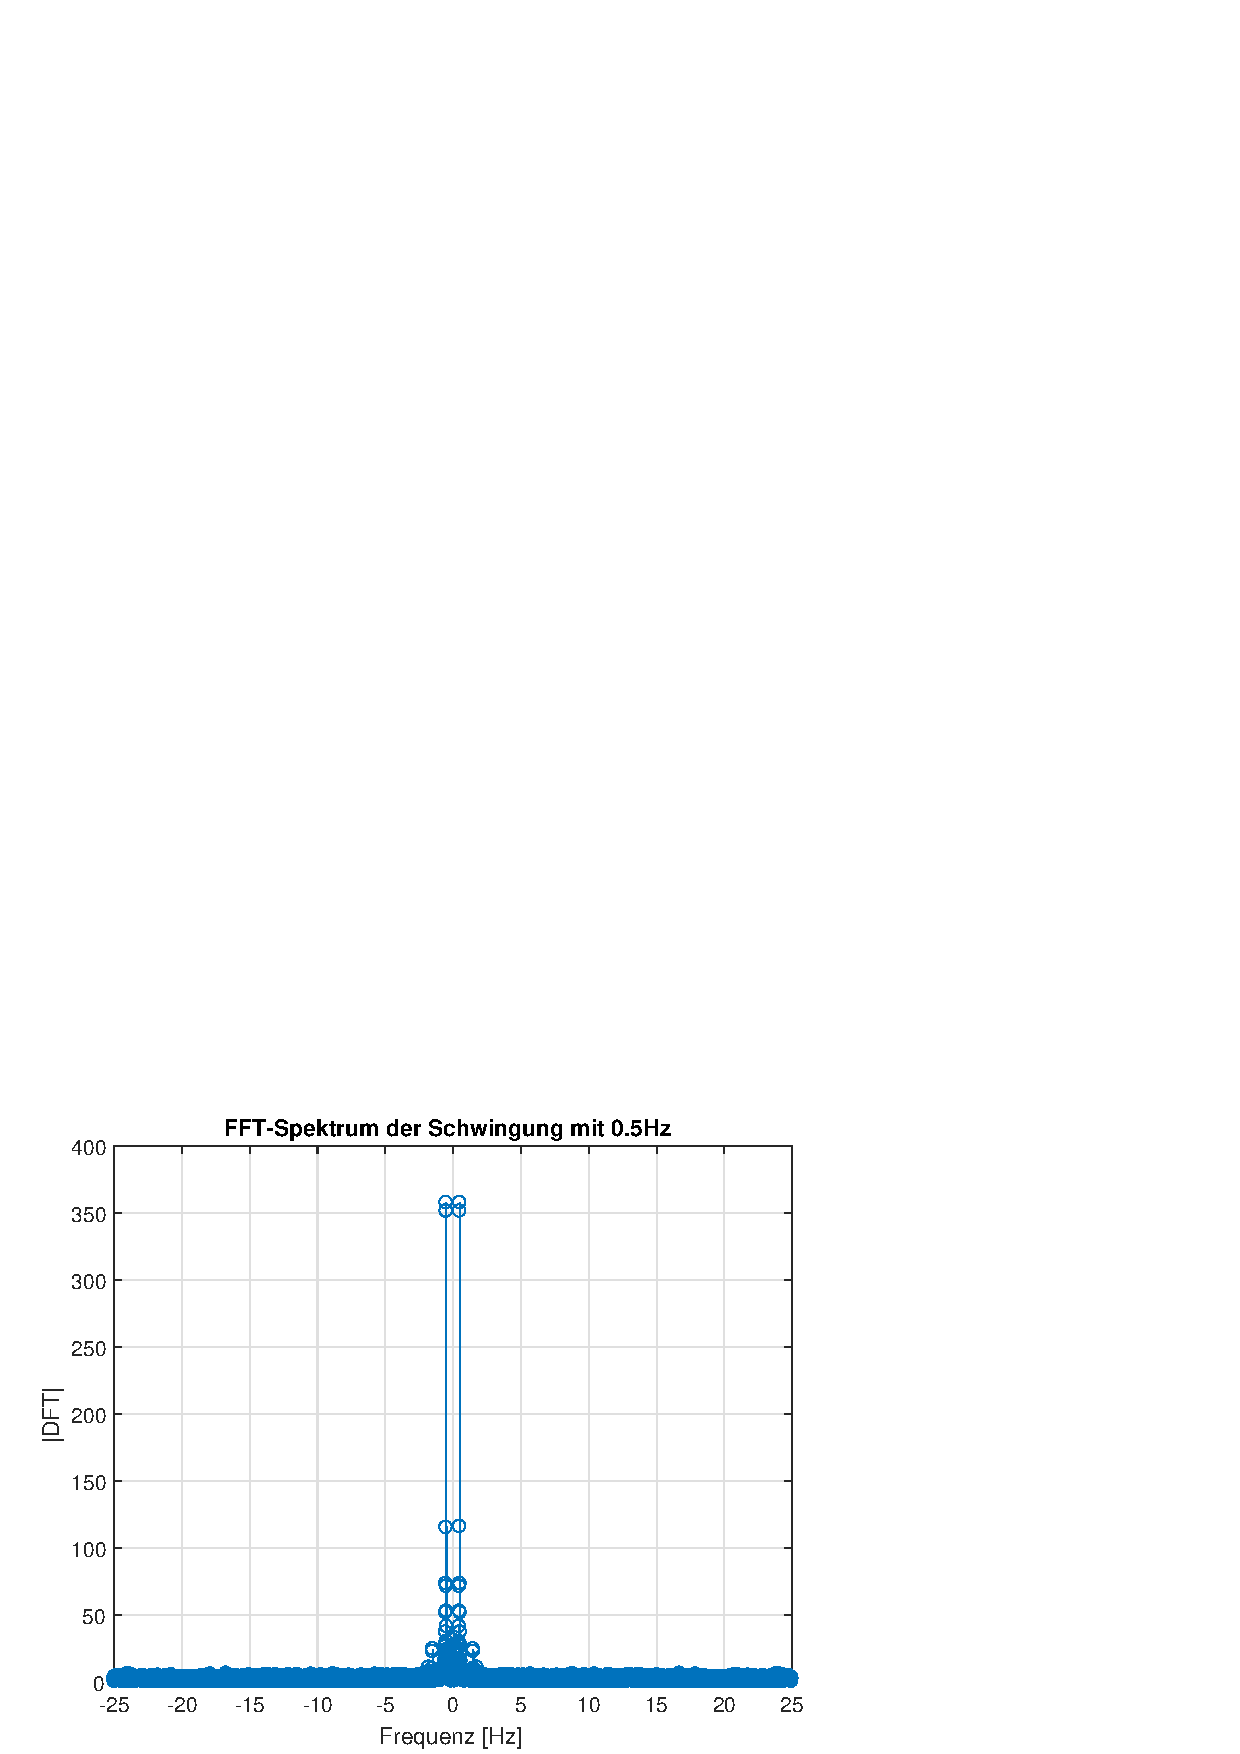
\includegraphics[width=0.5\linewidth]{img/dft_sinefreq_0_5}
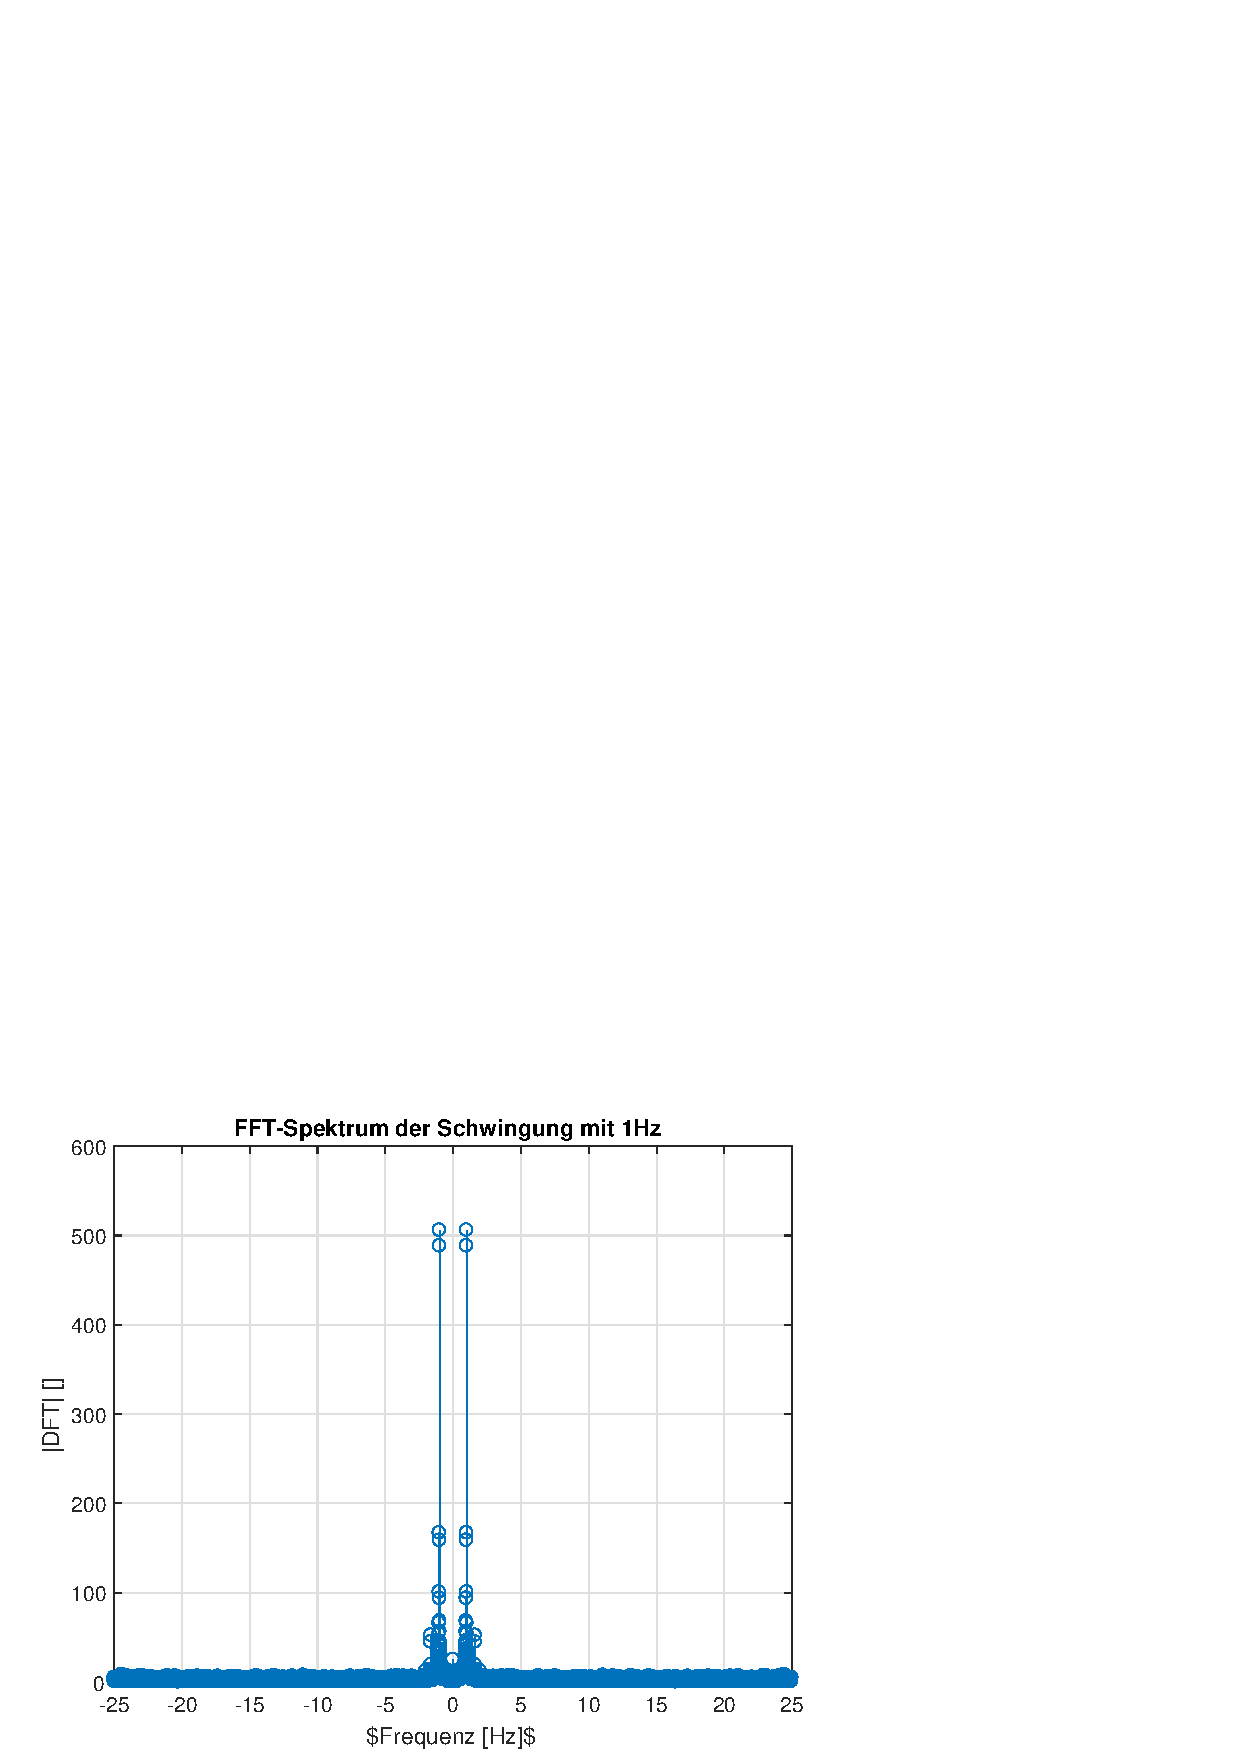
\includegraphics[width=0.5\linewidth]{img/dft_sinefreq_1}
\end{figure}
\begin{figure}[!h]
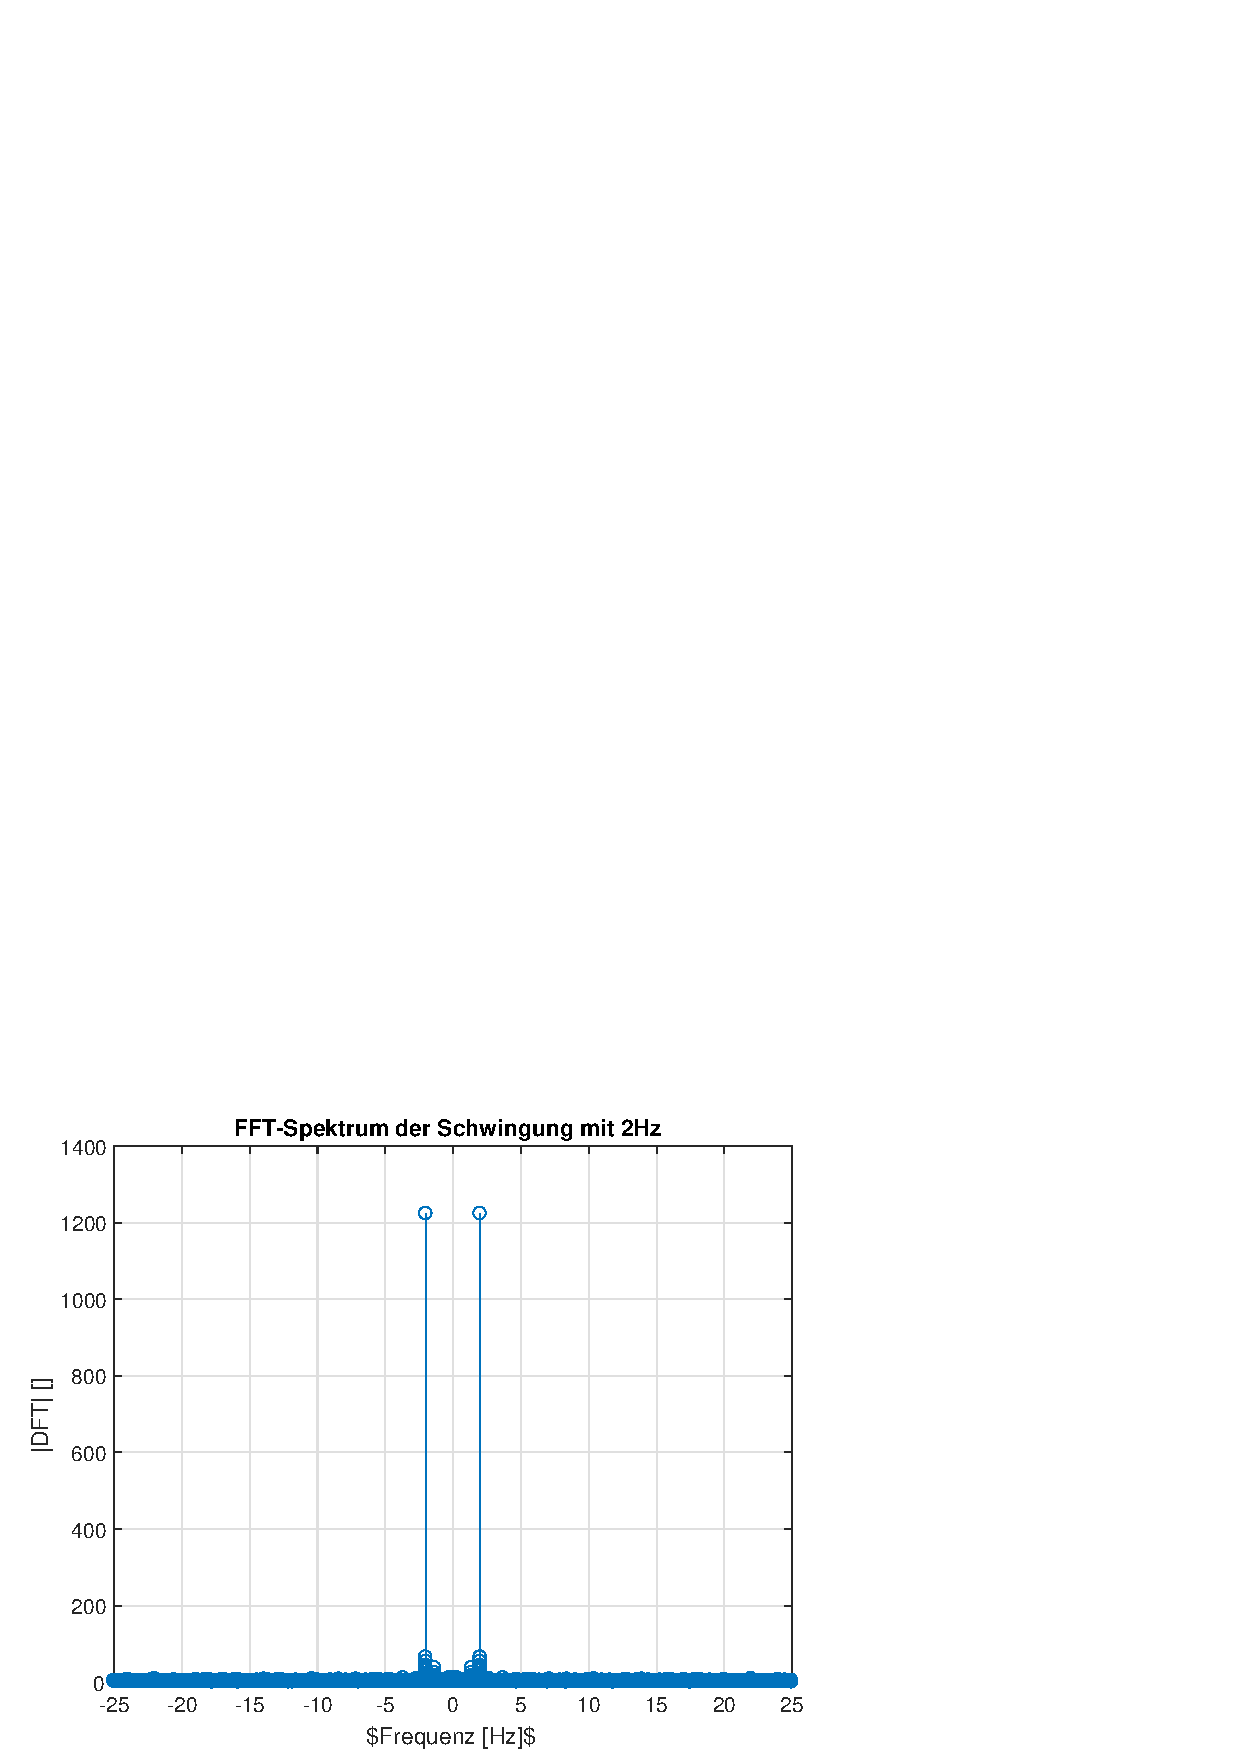
\includegraphics[width=0.5\linewidth]{img/dft_sinefreq_2}
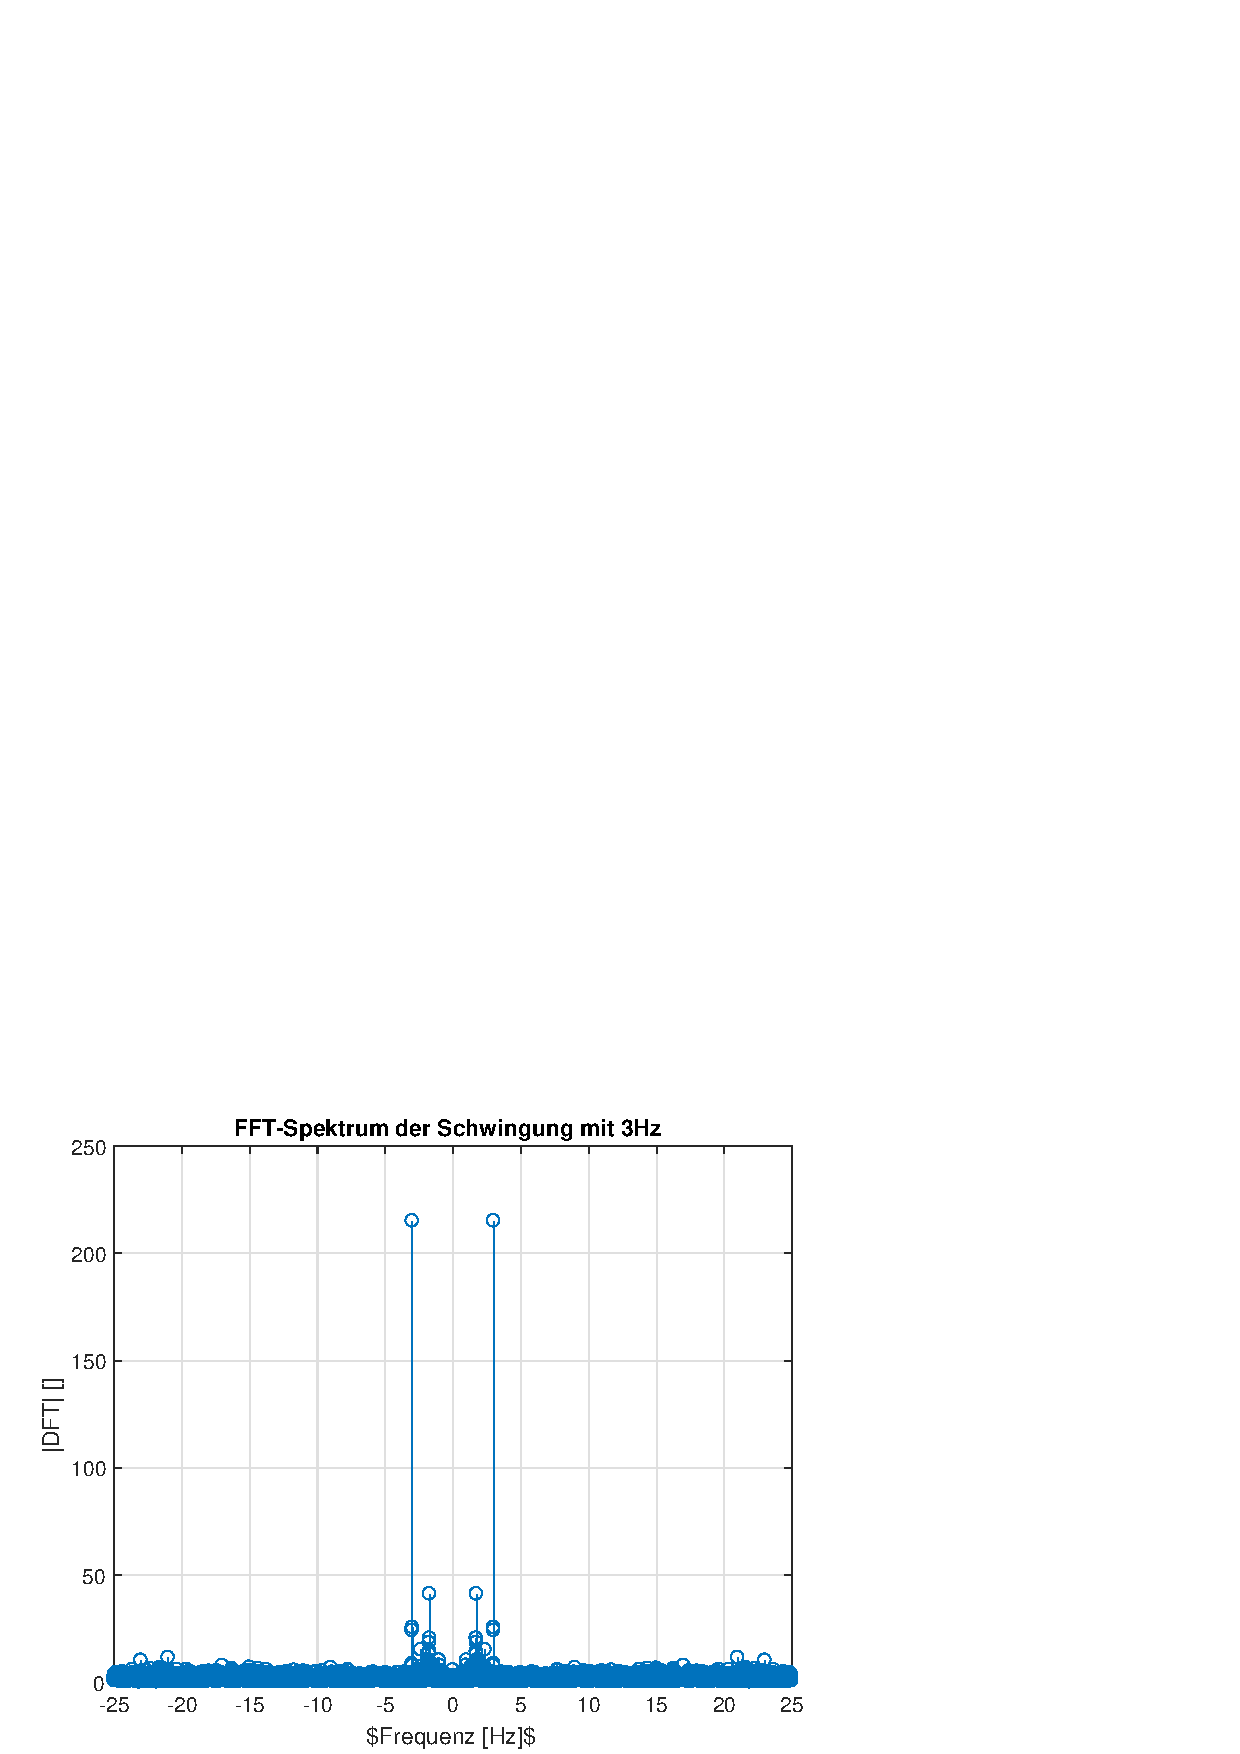
\includegraphics[width=0.5\linewidth]{img/dft_sinefreq_3}
\end{figure}
\begin{figure}[!h]
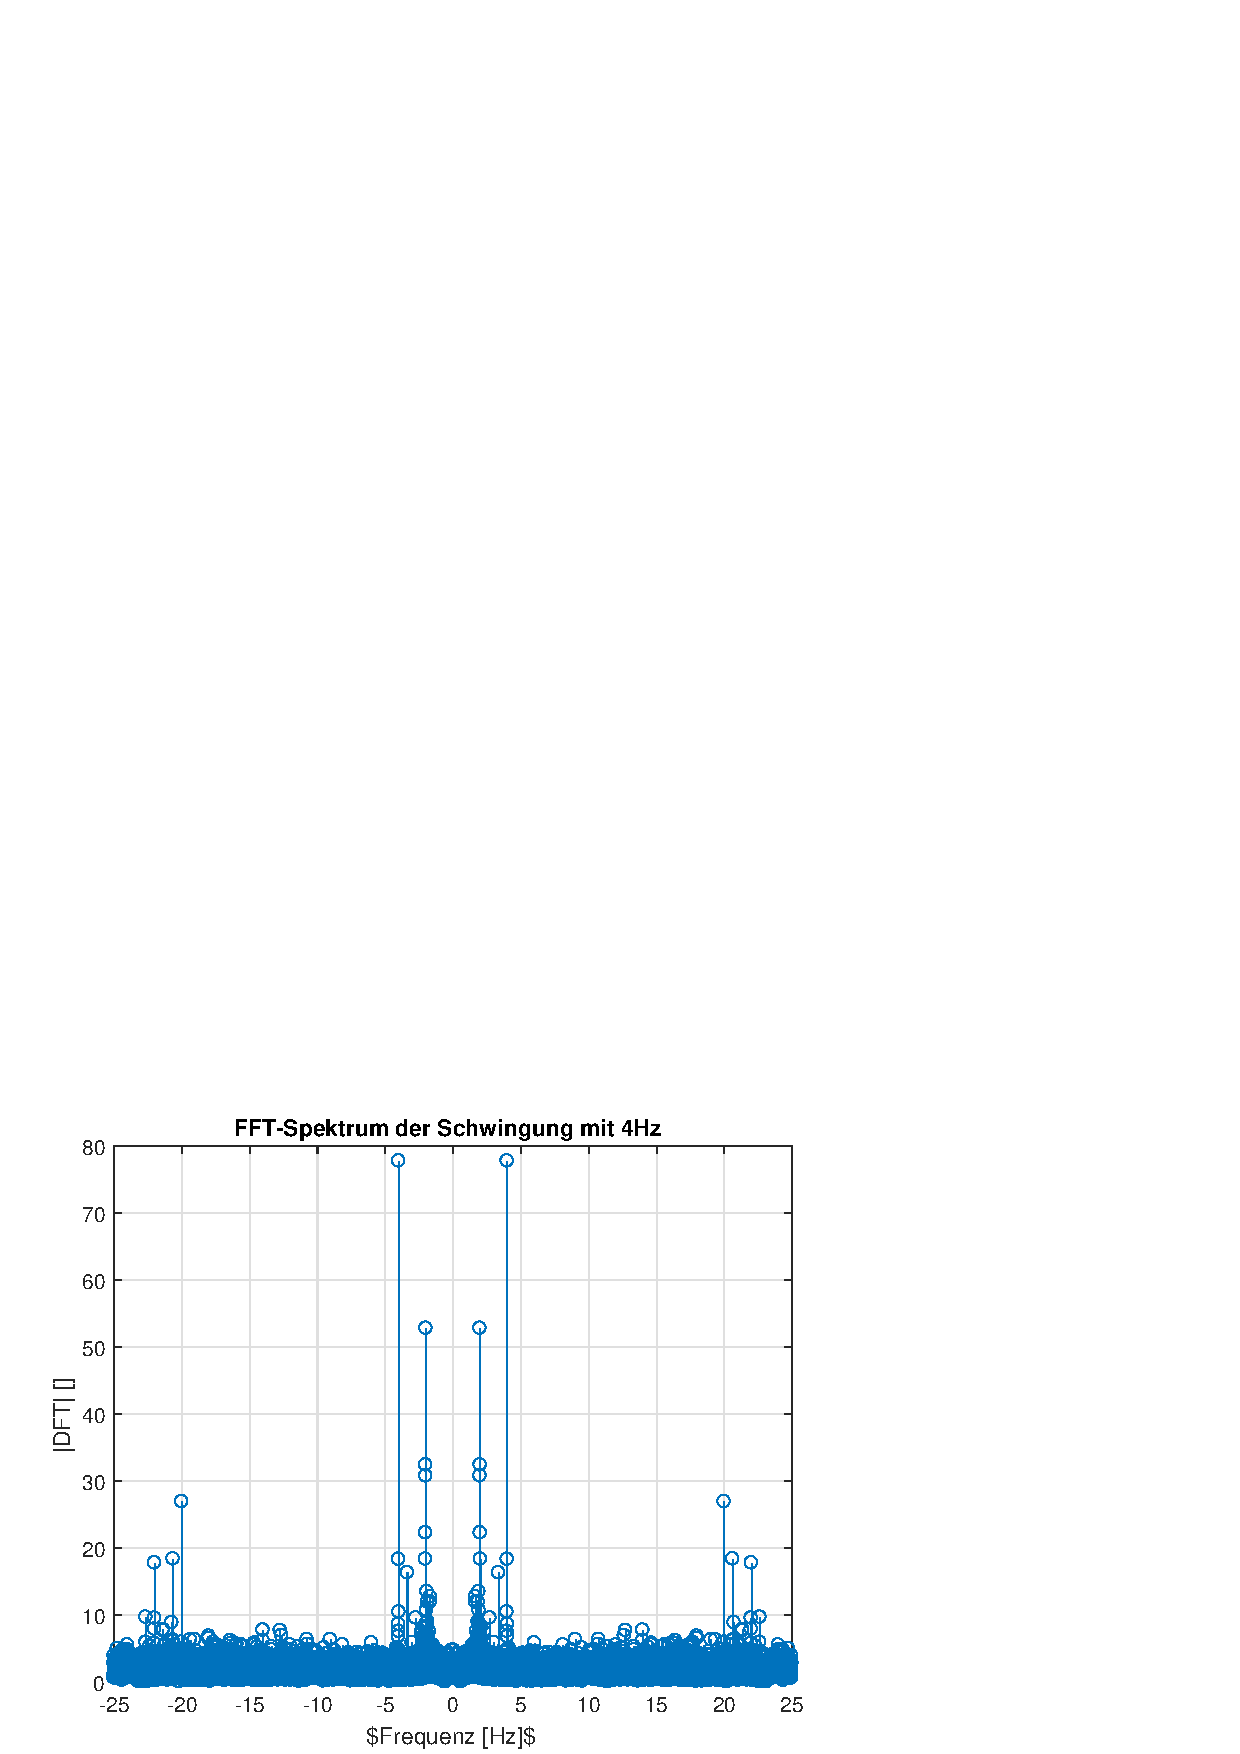
\includegraphics[width=0.5\linewidth]{img/dft_sinefreq_4}
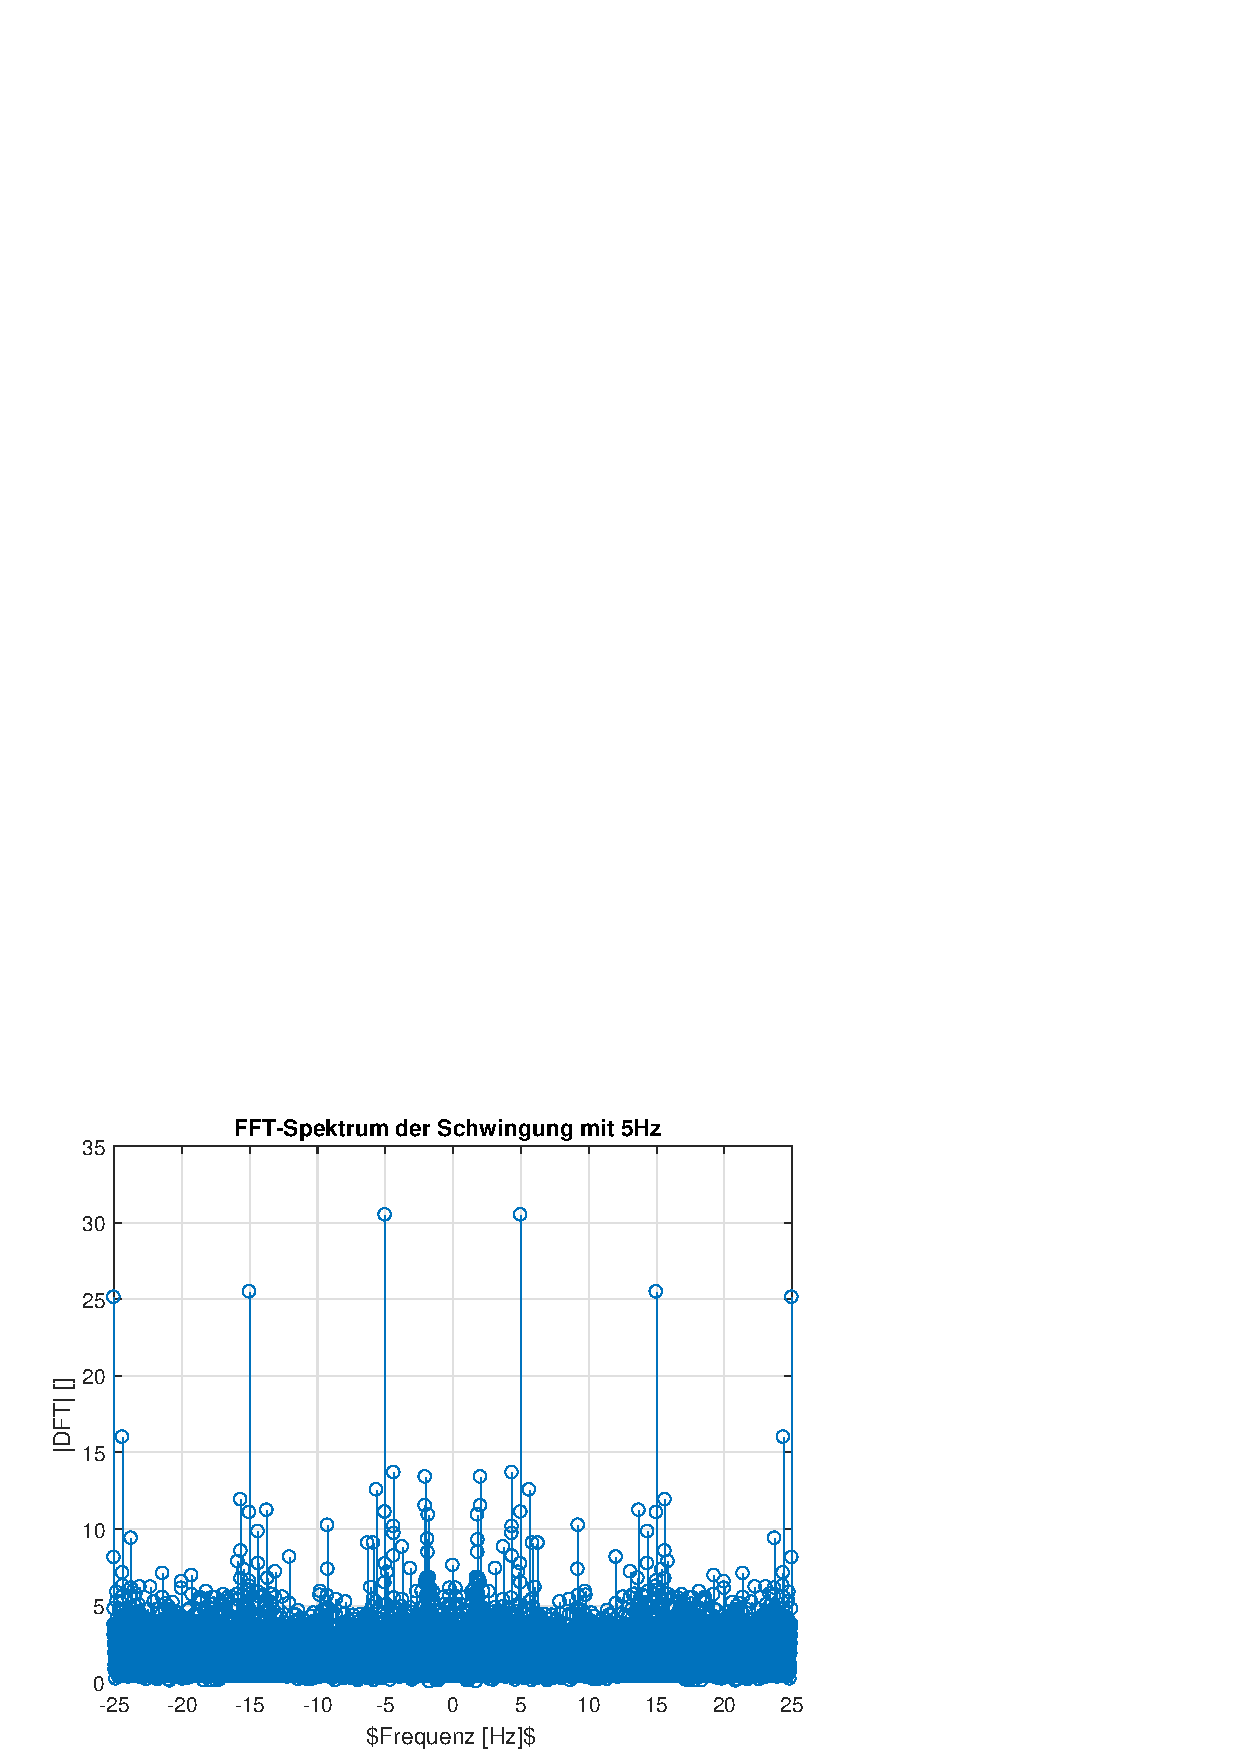
\includegraphics[width=0.5\linewidth]{img/dft_sinefreq_5}
\end{figure}
\begin{figure}[!h]
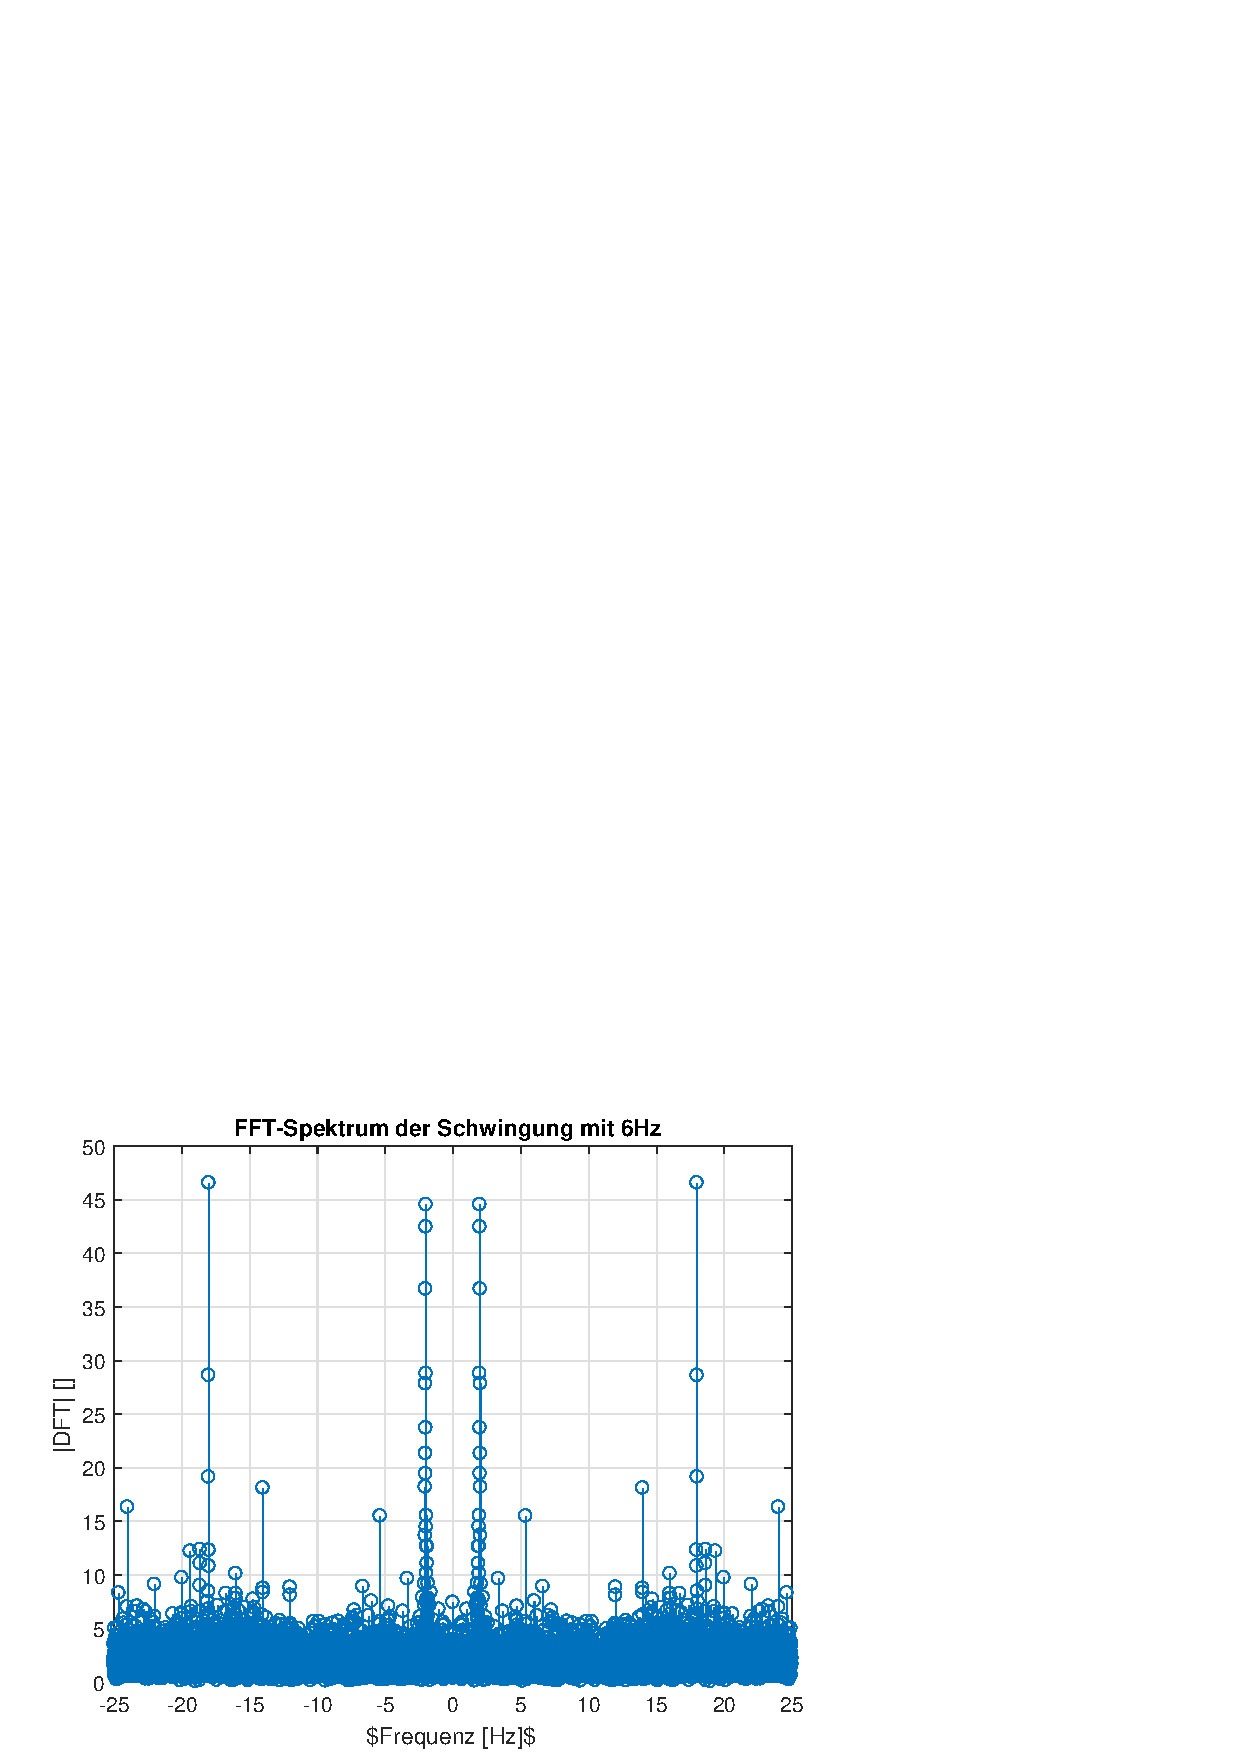
\includegraphics[width=0.5\linewidth]{img/dft_sinefreq_6}
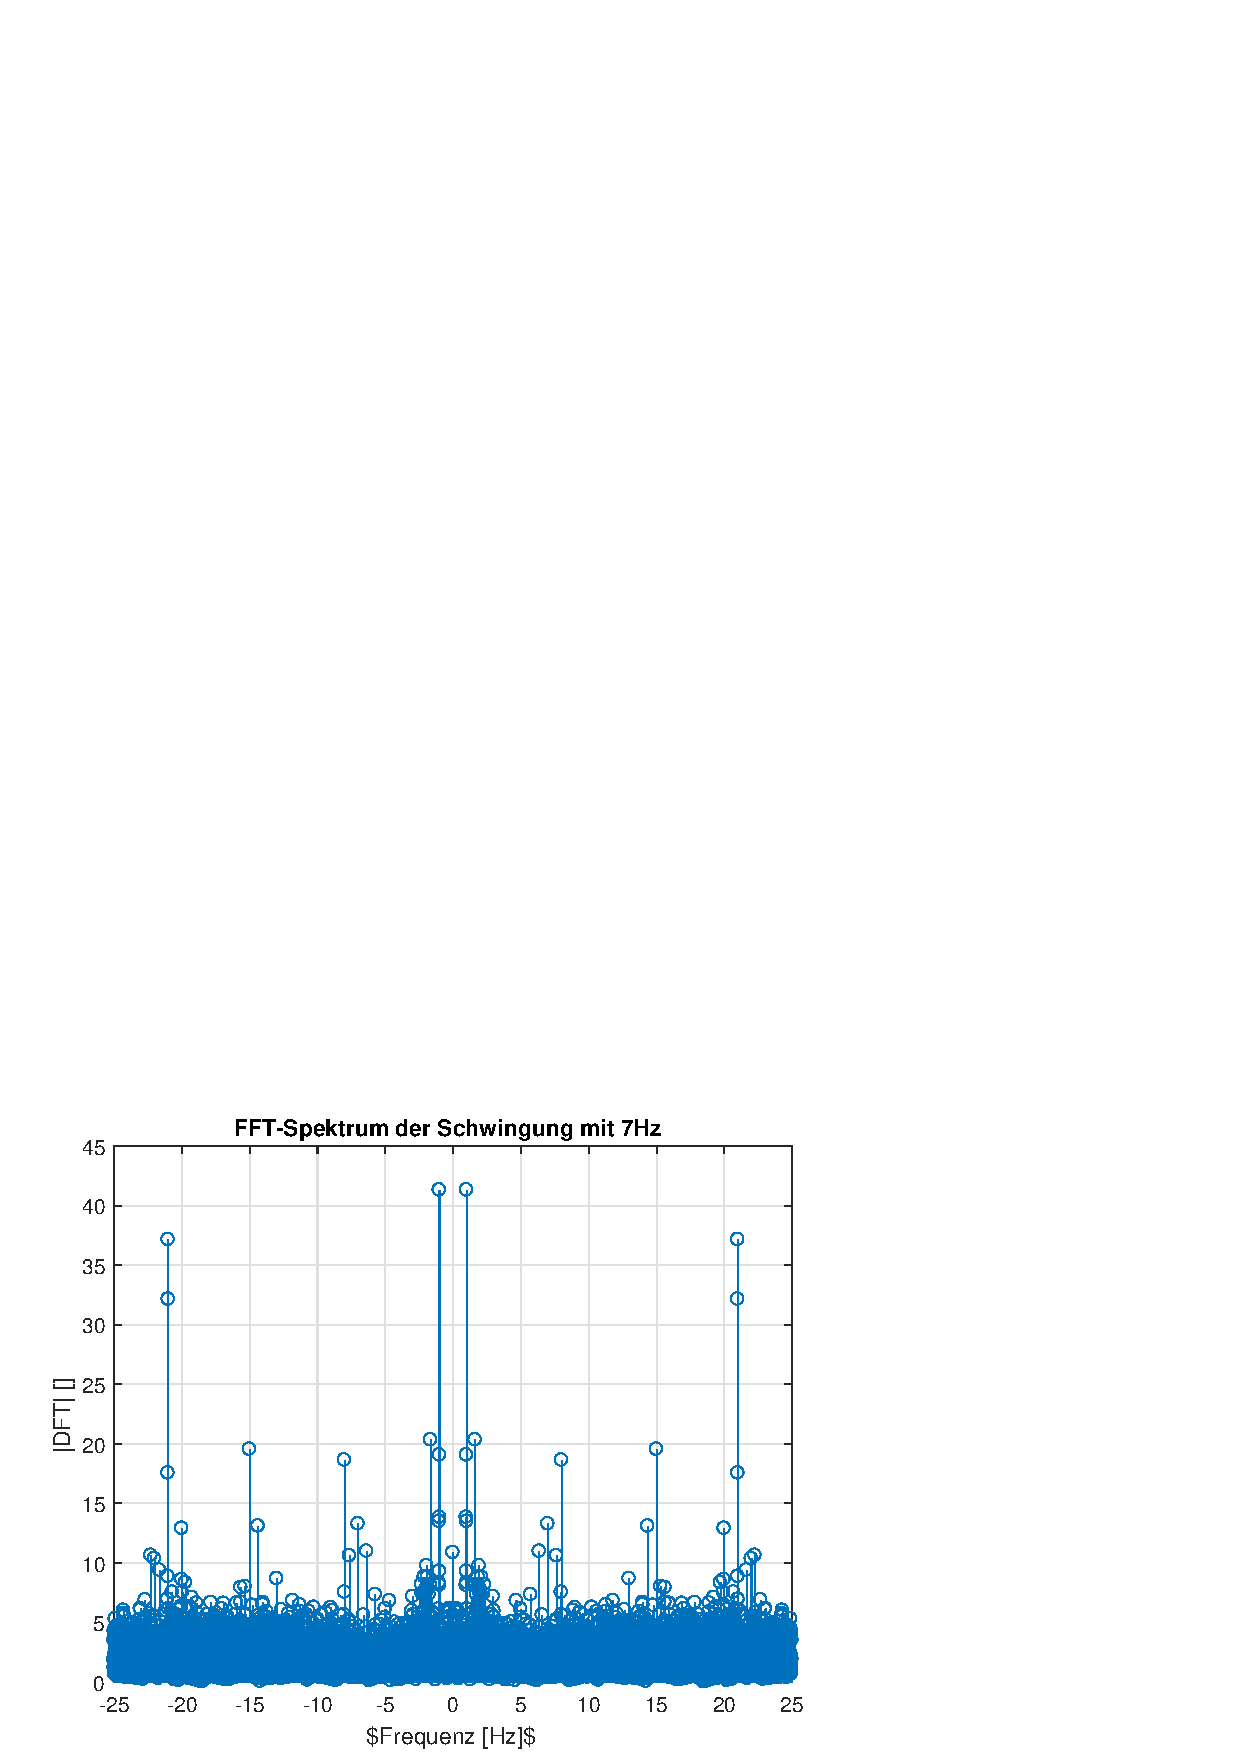
\includegraphics[width=0.5\linewidth]{img/dft_sinefreq_7}
\end{figure}
\begin{figure}[!h]
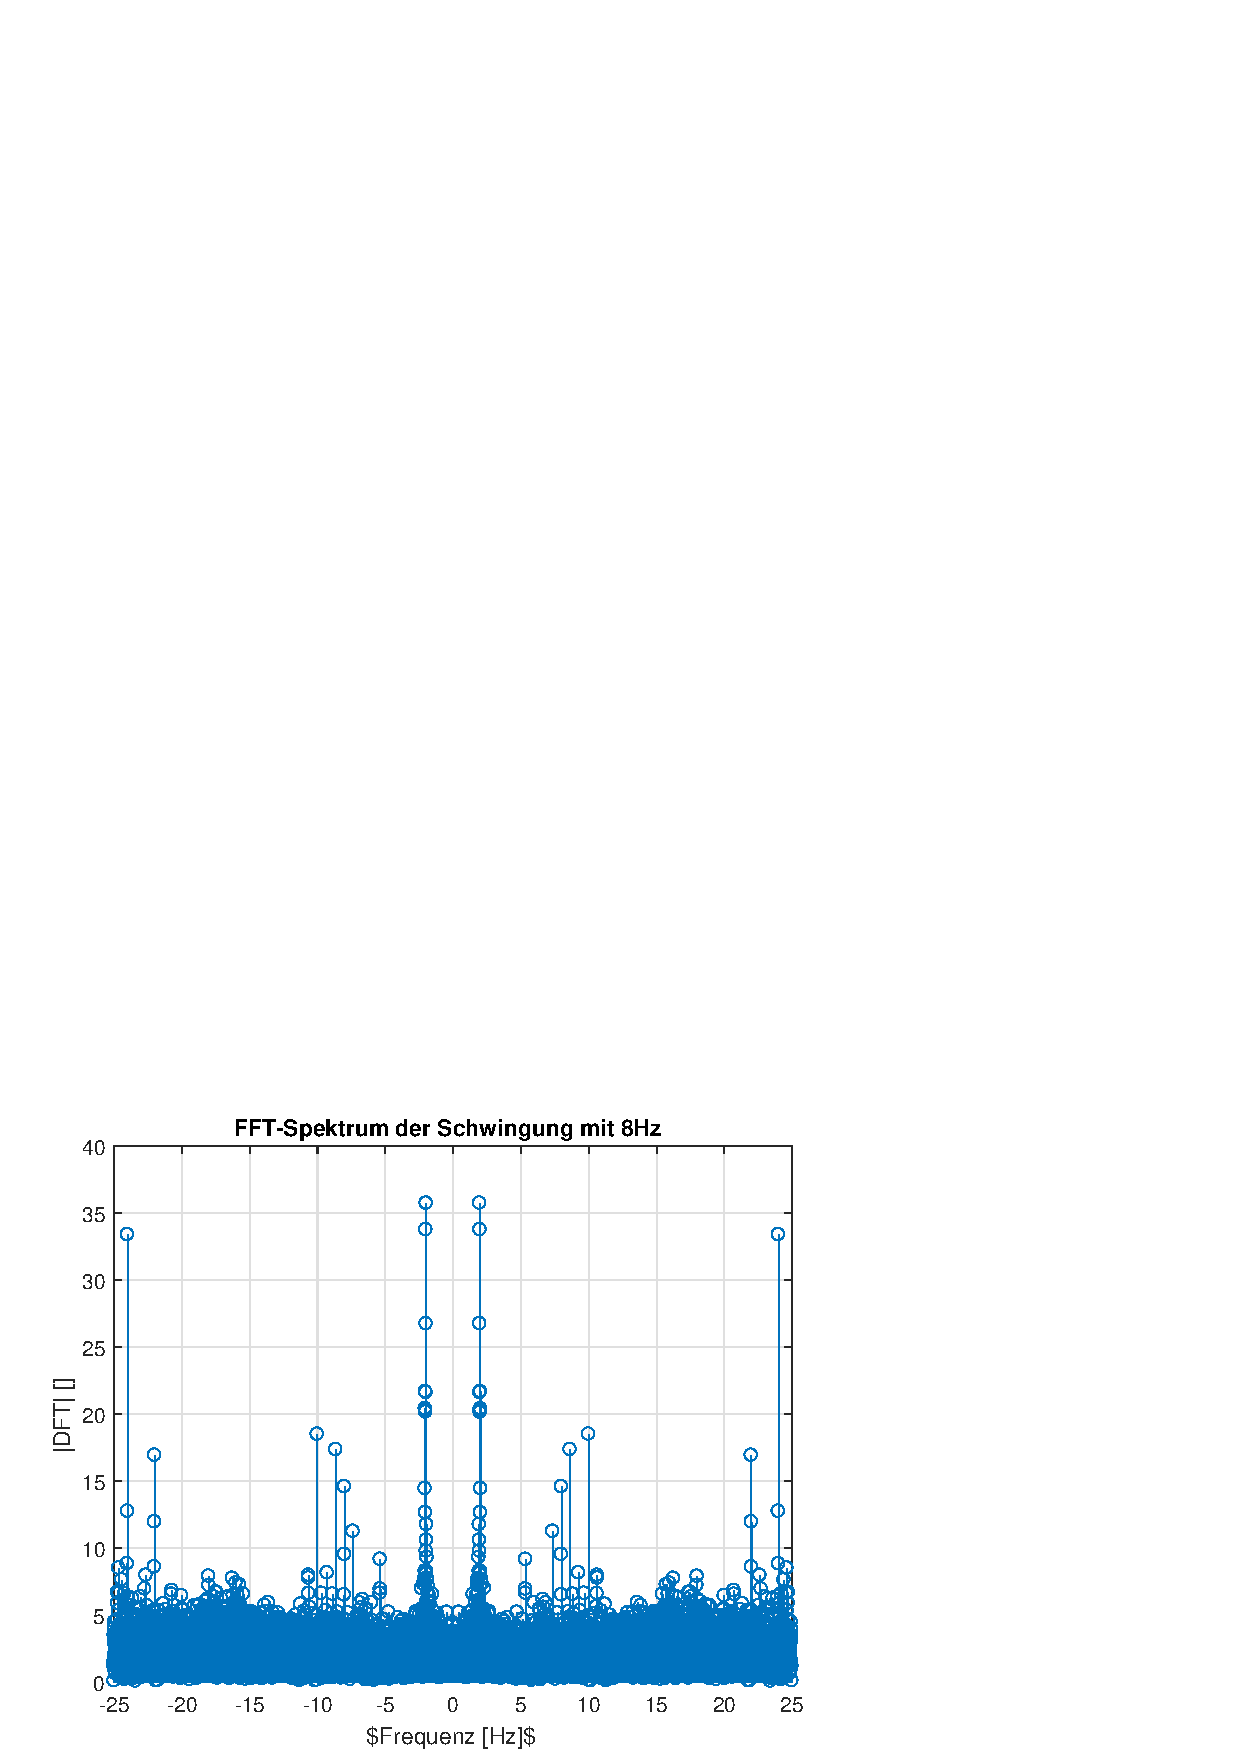
\includegraphics[width=0.5\linewidth]{img/dft_sinefreq_8}
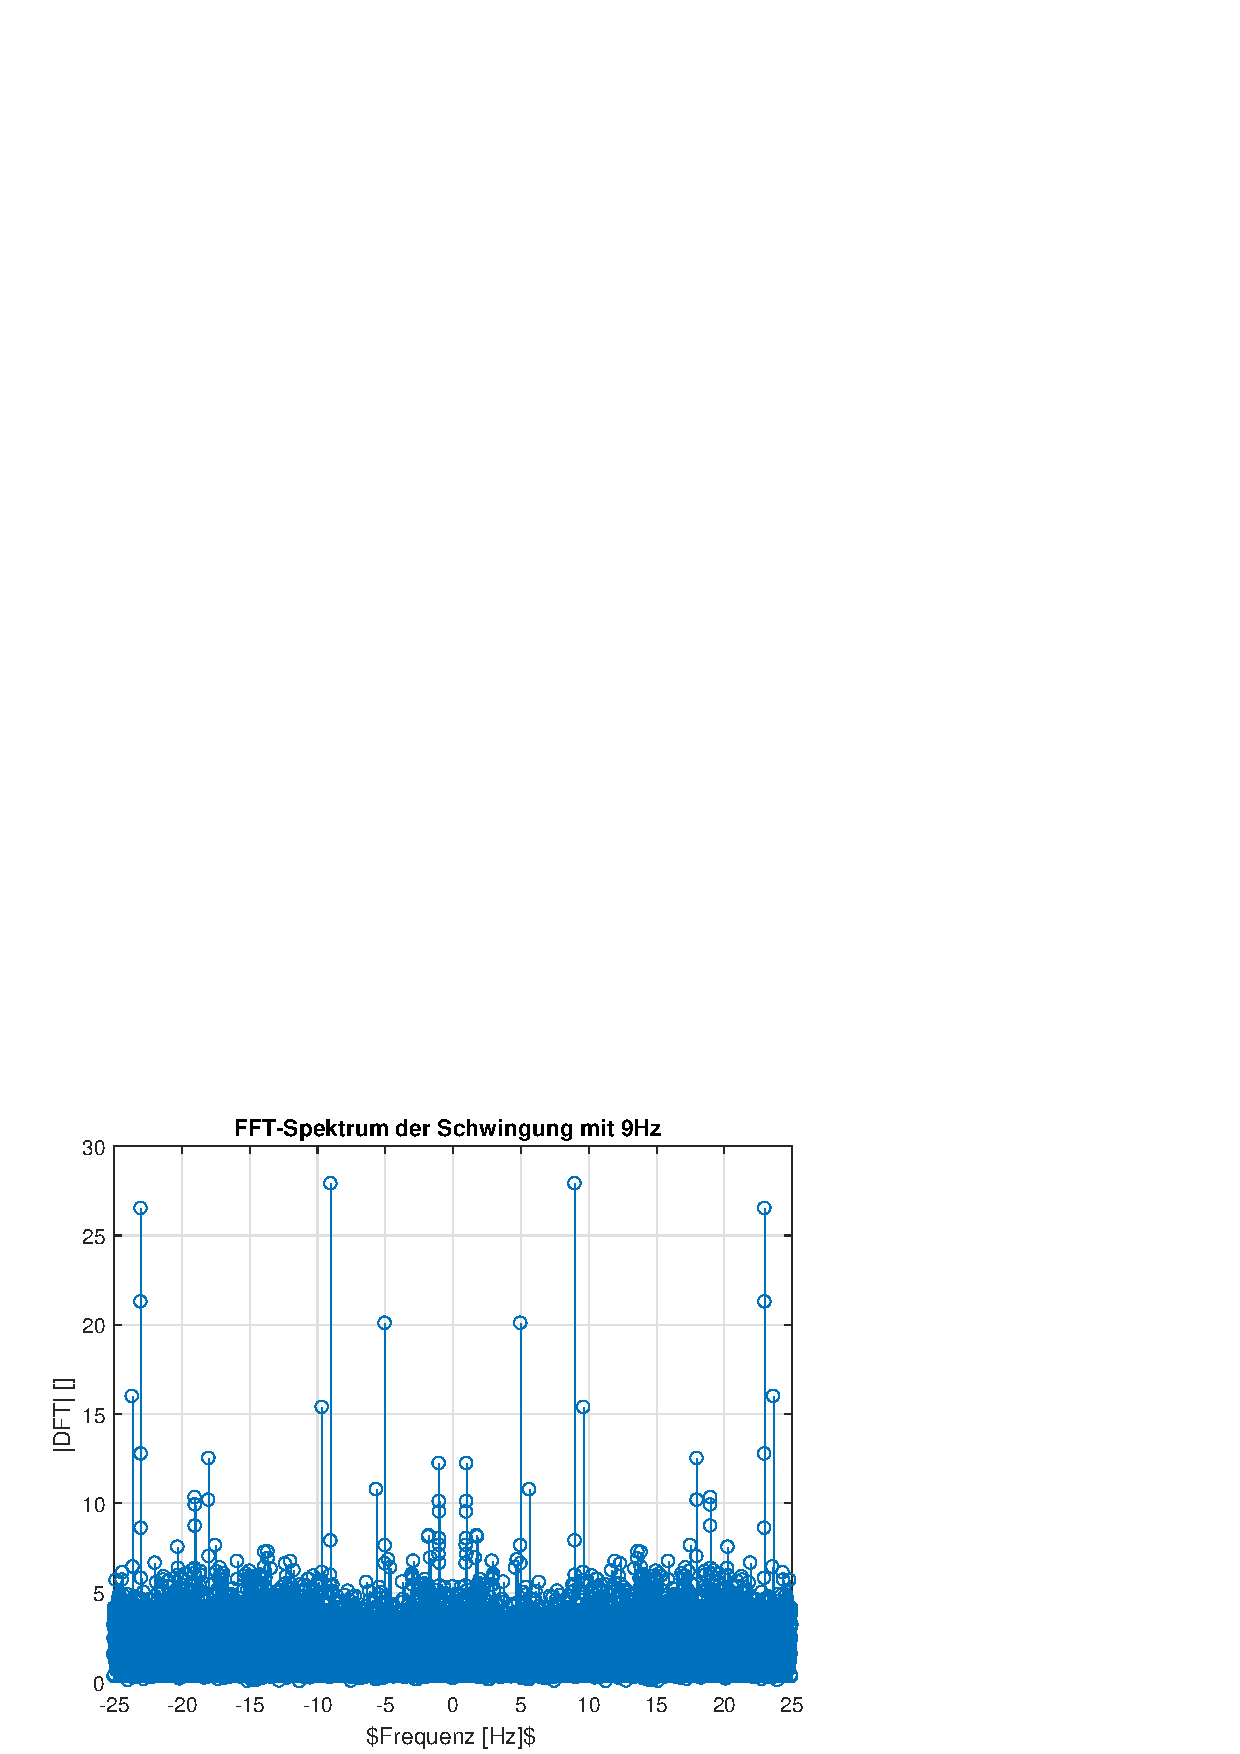
\includegraphics[width=0.5\linewidth]{img/dft_sinefreq_9}
\end{figure}
\begin{figure}[!h]
\centering
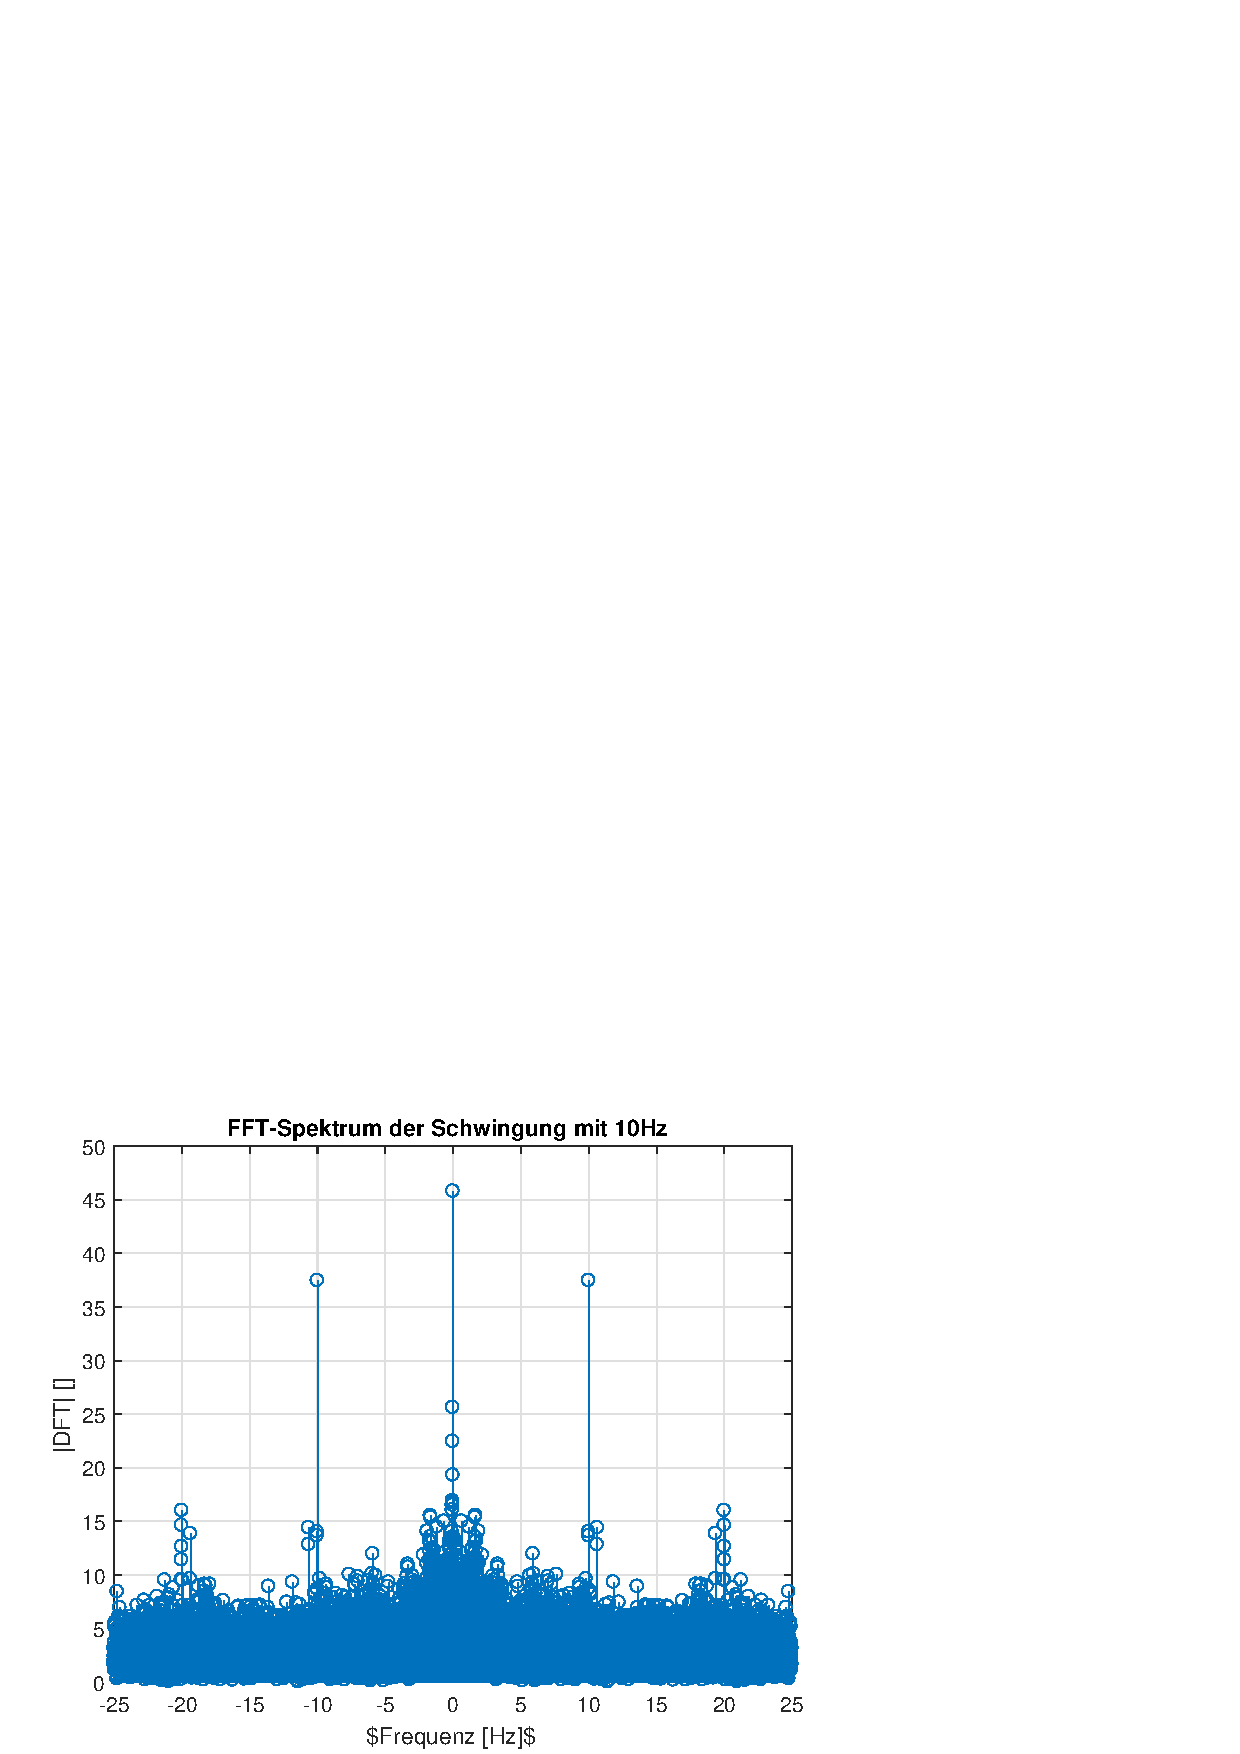
\includegraphics[width=0.5\linewidth]{img/dft_sinefreq_10}
\end{figure}

\newpage
\subsubsection{Autokorelleation von $\varphi$ bei $T_M = sin(2\pi\cdot f\cdot t)$}
\begin{figure}[!h]
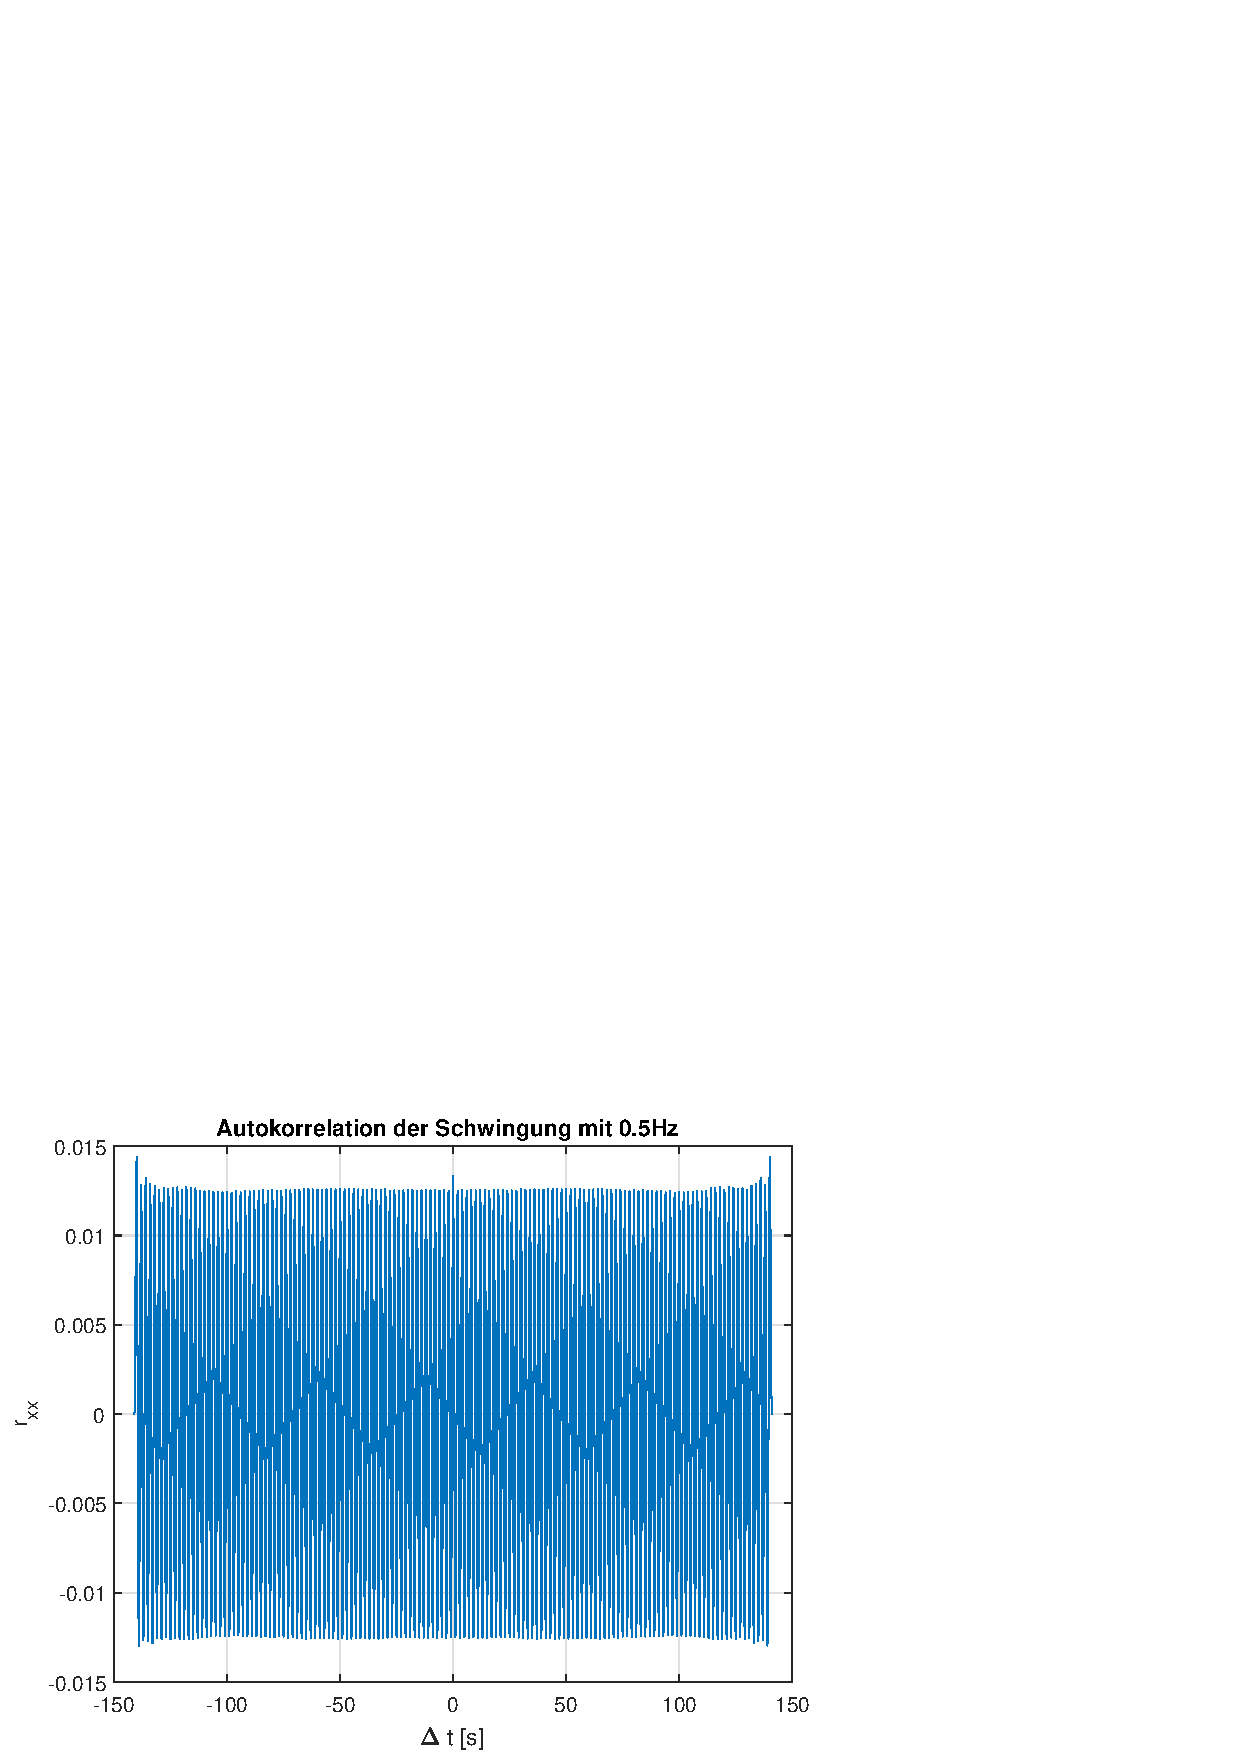
\includegraphics[width=0.5\linewidth]{img/rxx_sinefreq_0_5}
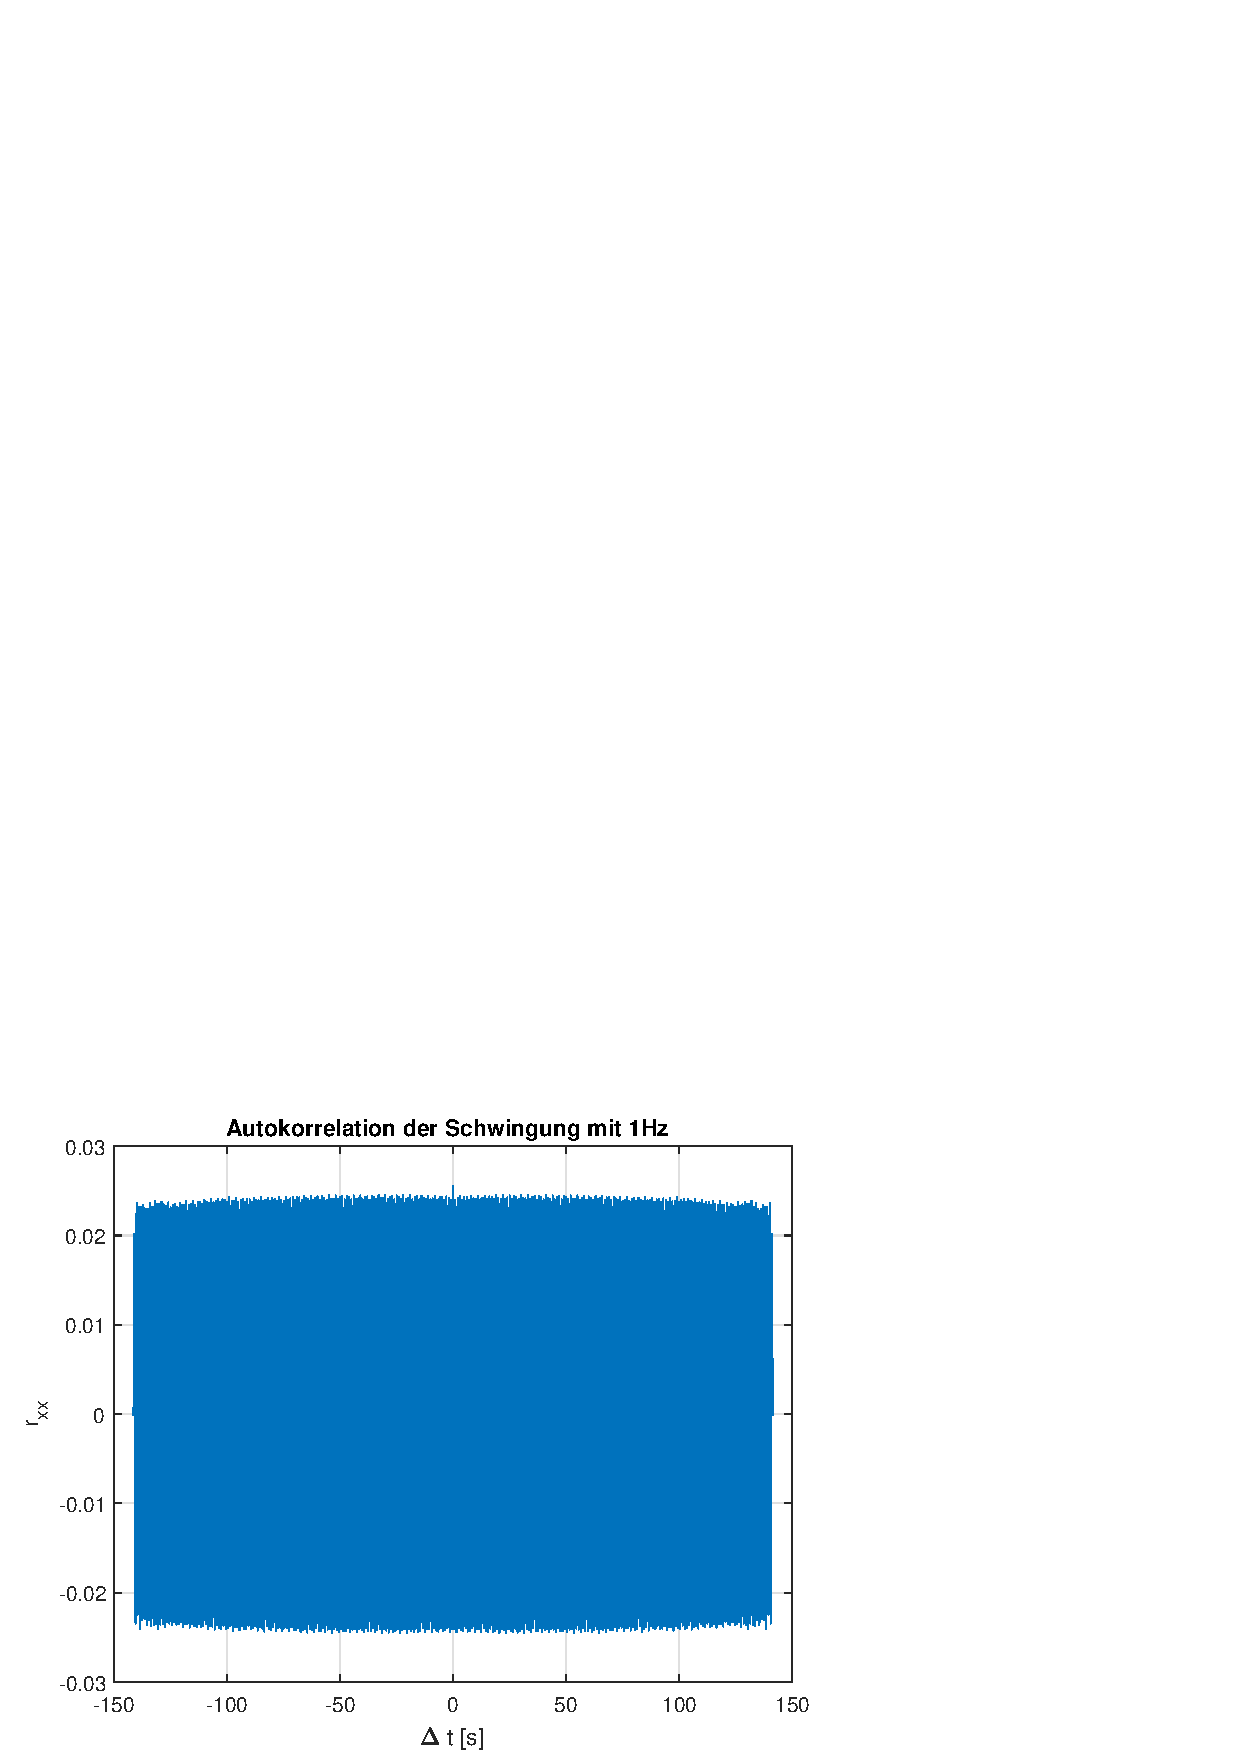
\includegraphics[width=0.5\linewidth]{img/rxx_sinefreq_1}
\end{figure}
\begin{figure}[!h]
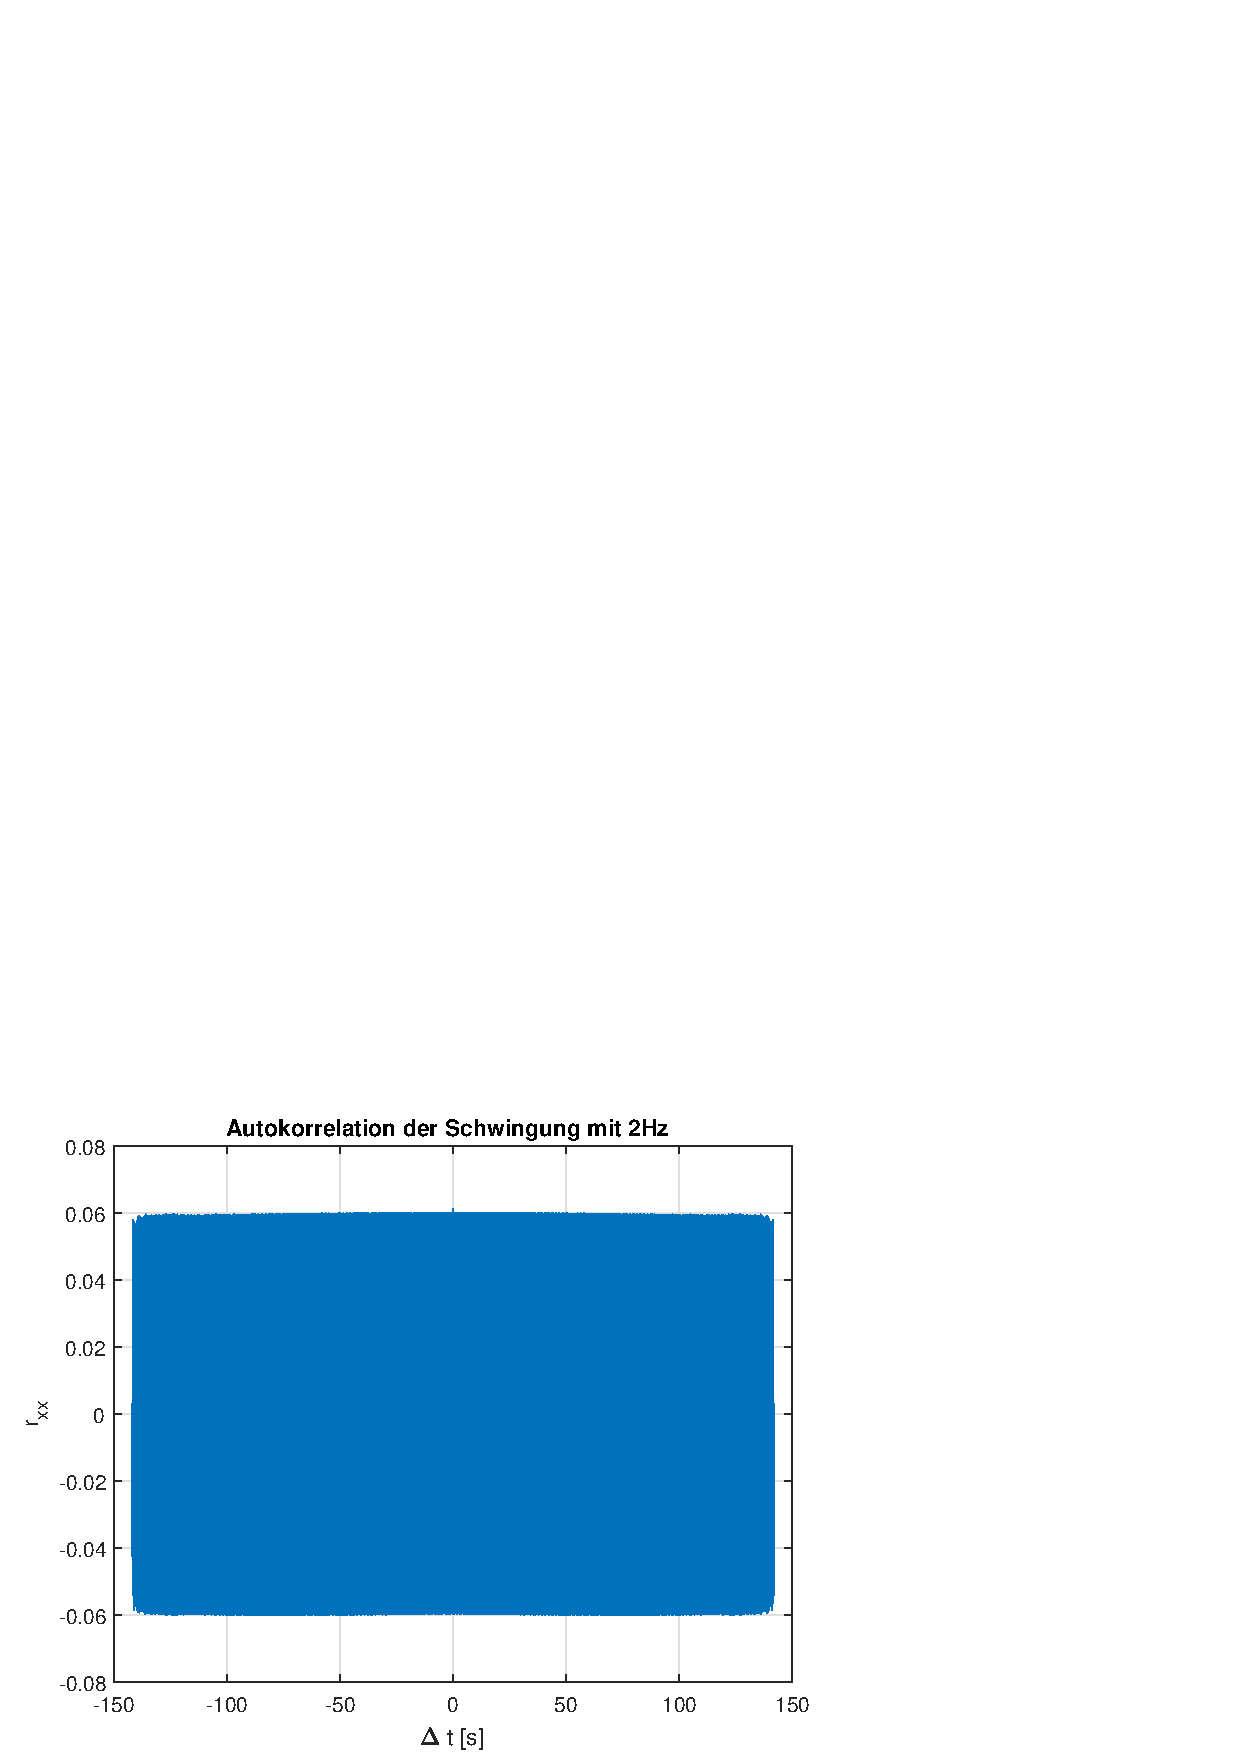
\includegraphics[width=0.5\linewidth]{img/rxx_sinefreq_2}
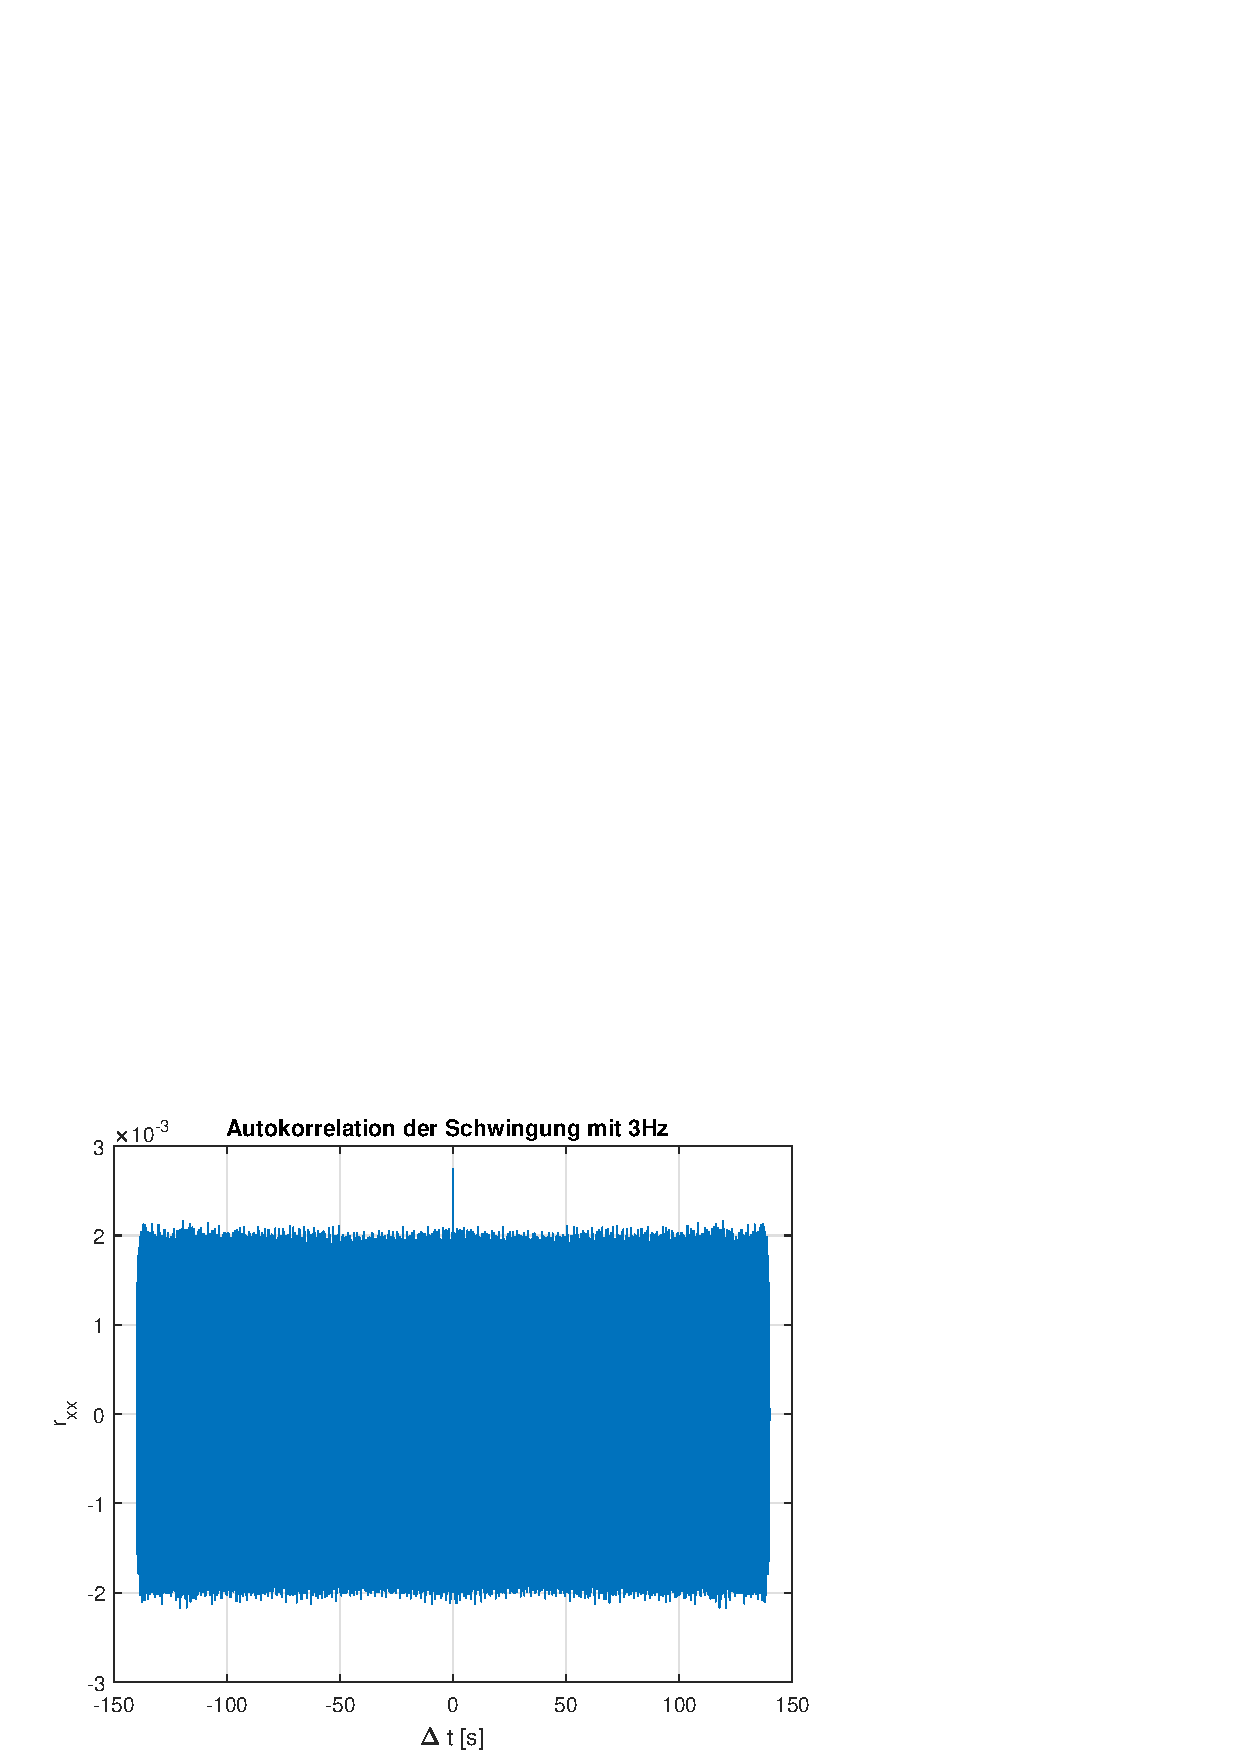
\includegraphics[width=0.5\linewidth]{img/rxx_sinefreq_3}
\end{figure}
\begin{figure}[!h]
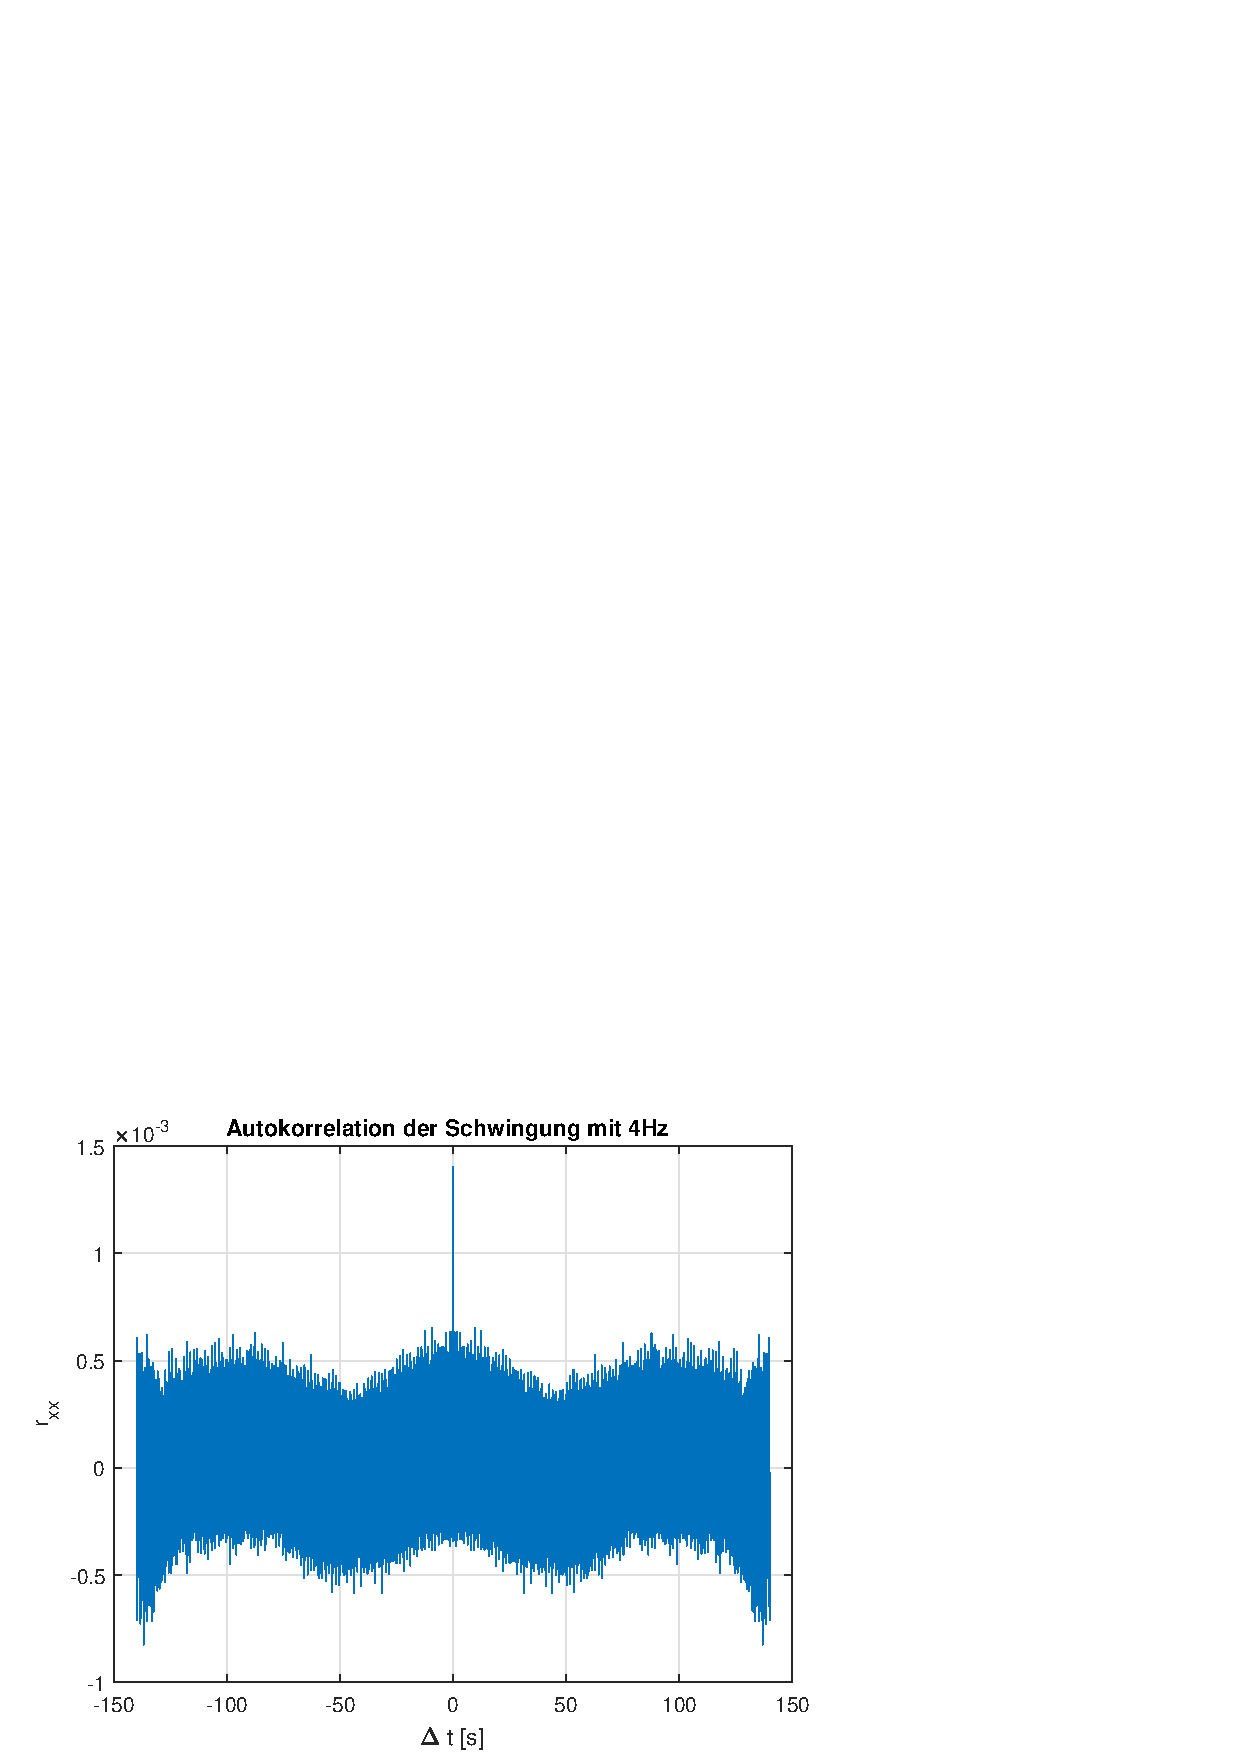
\includegraphics[width=0.5\linewidth]{img/rxx_sinefreq_4}
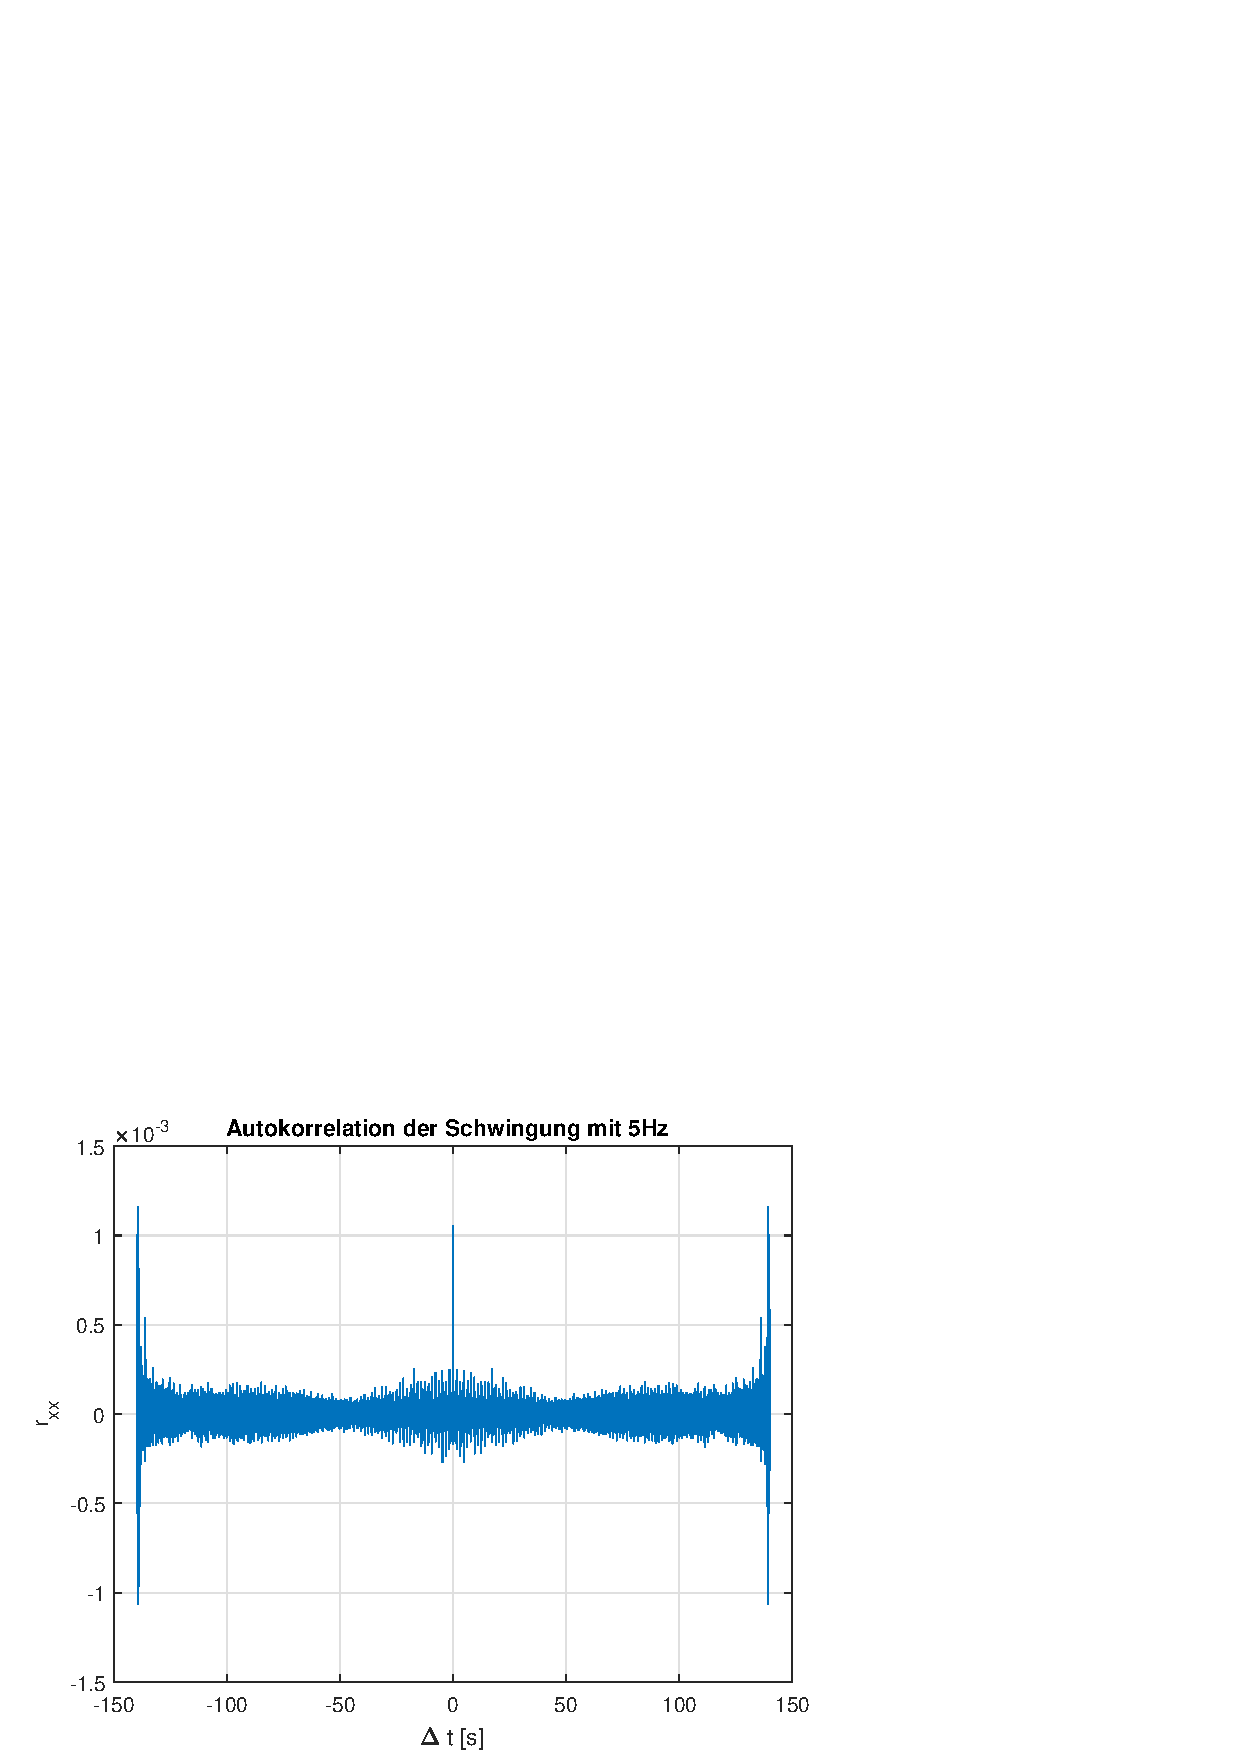
\includegraphics[width=0.5\linewidth]{img/rxx_sinefreq_5}
\end{figure}
\begin{figure}[!h]
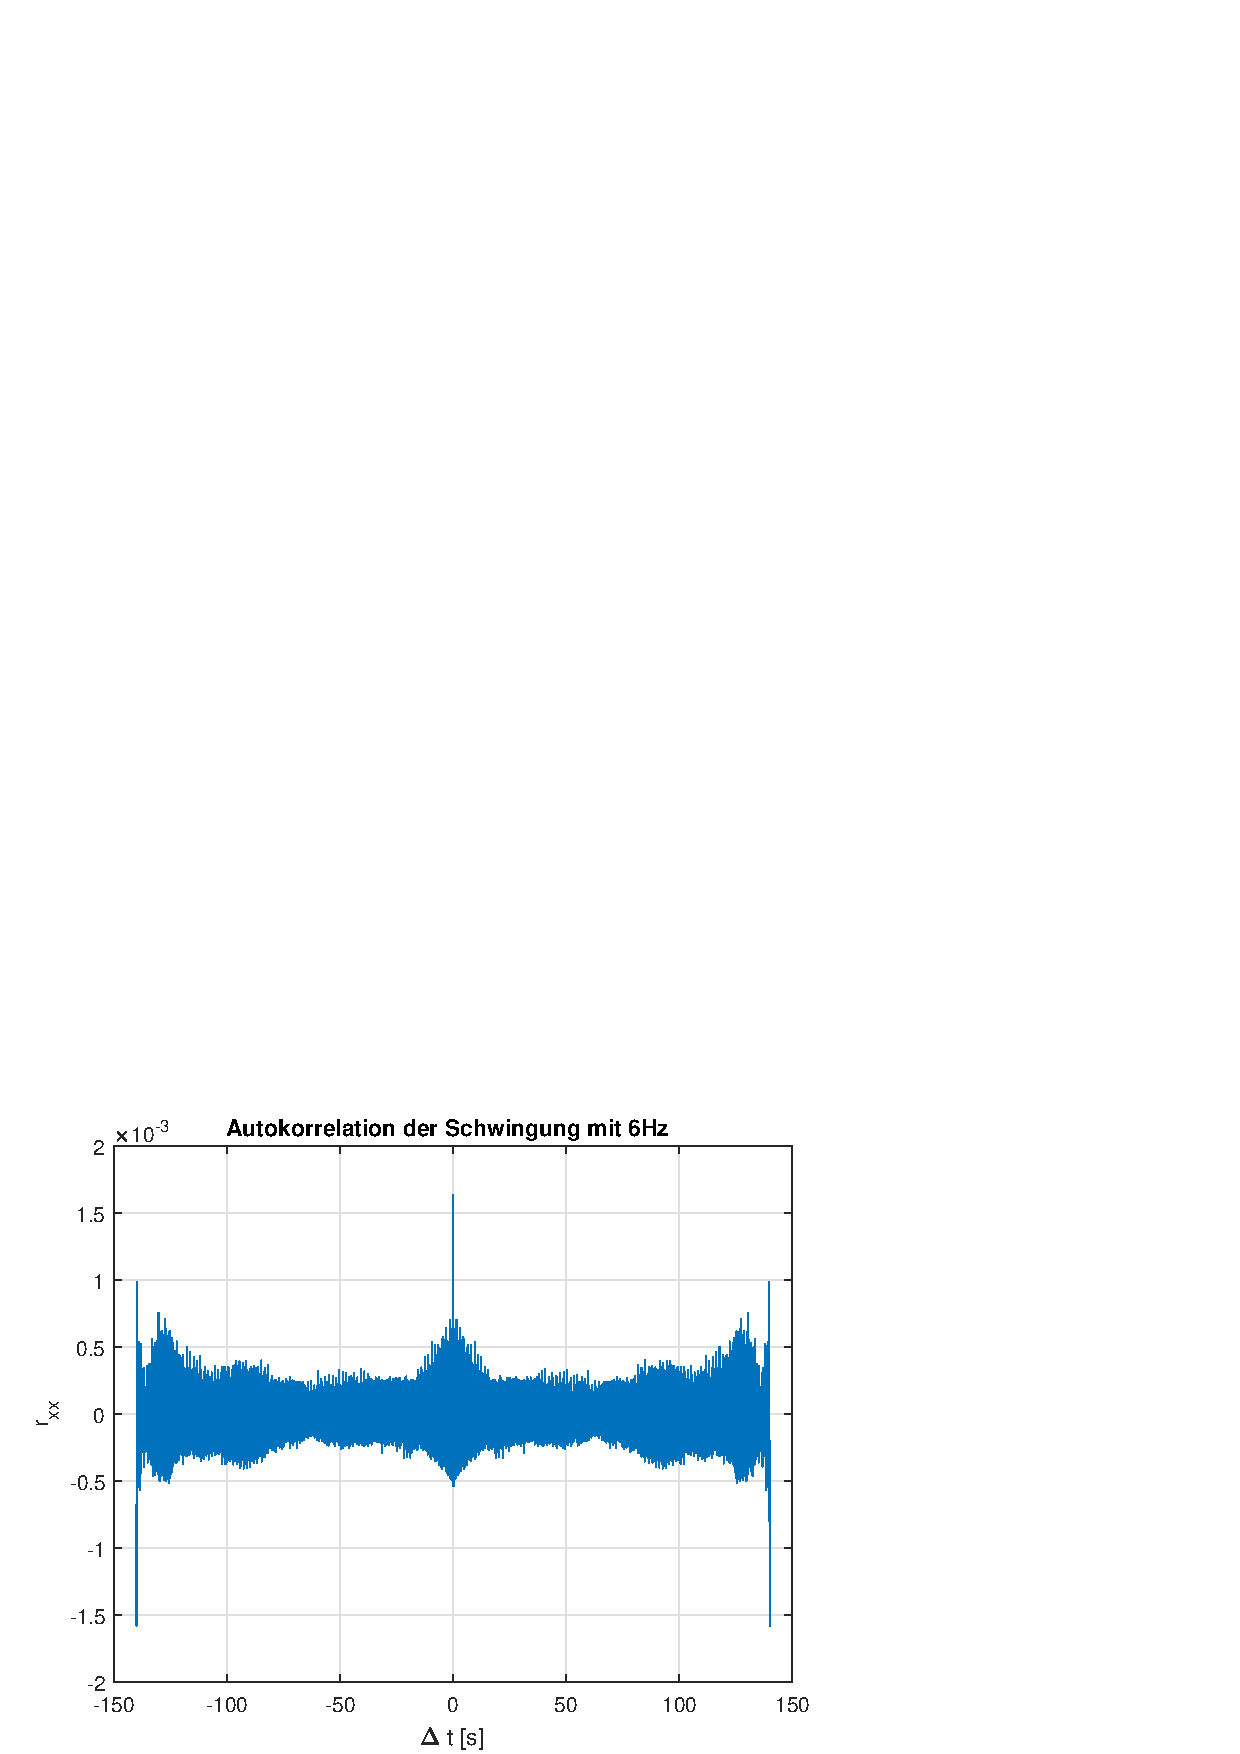
\includegraphics[width=0.5\linewidth]{img/rxx_sinefreq_6}
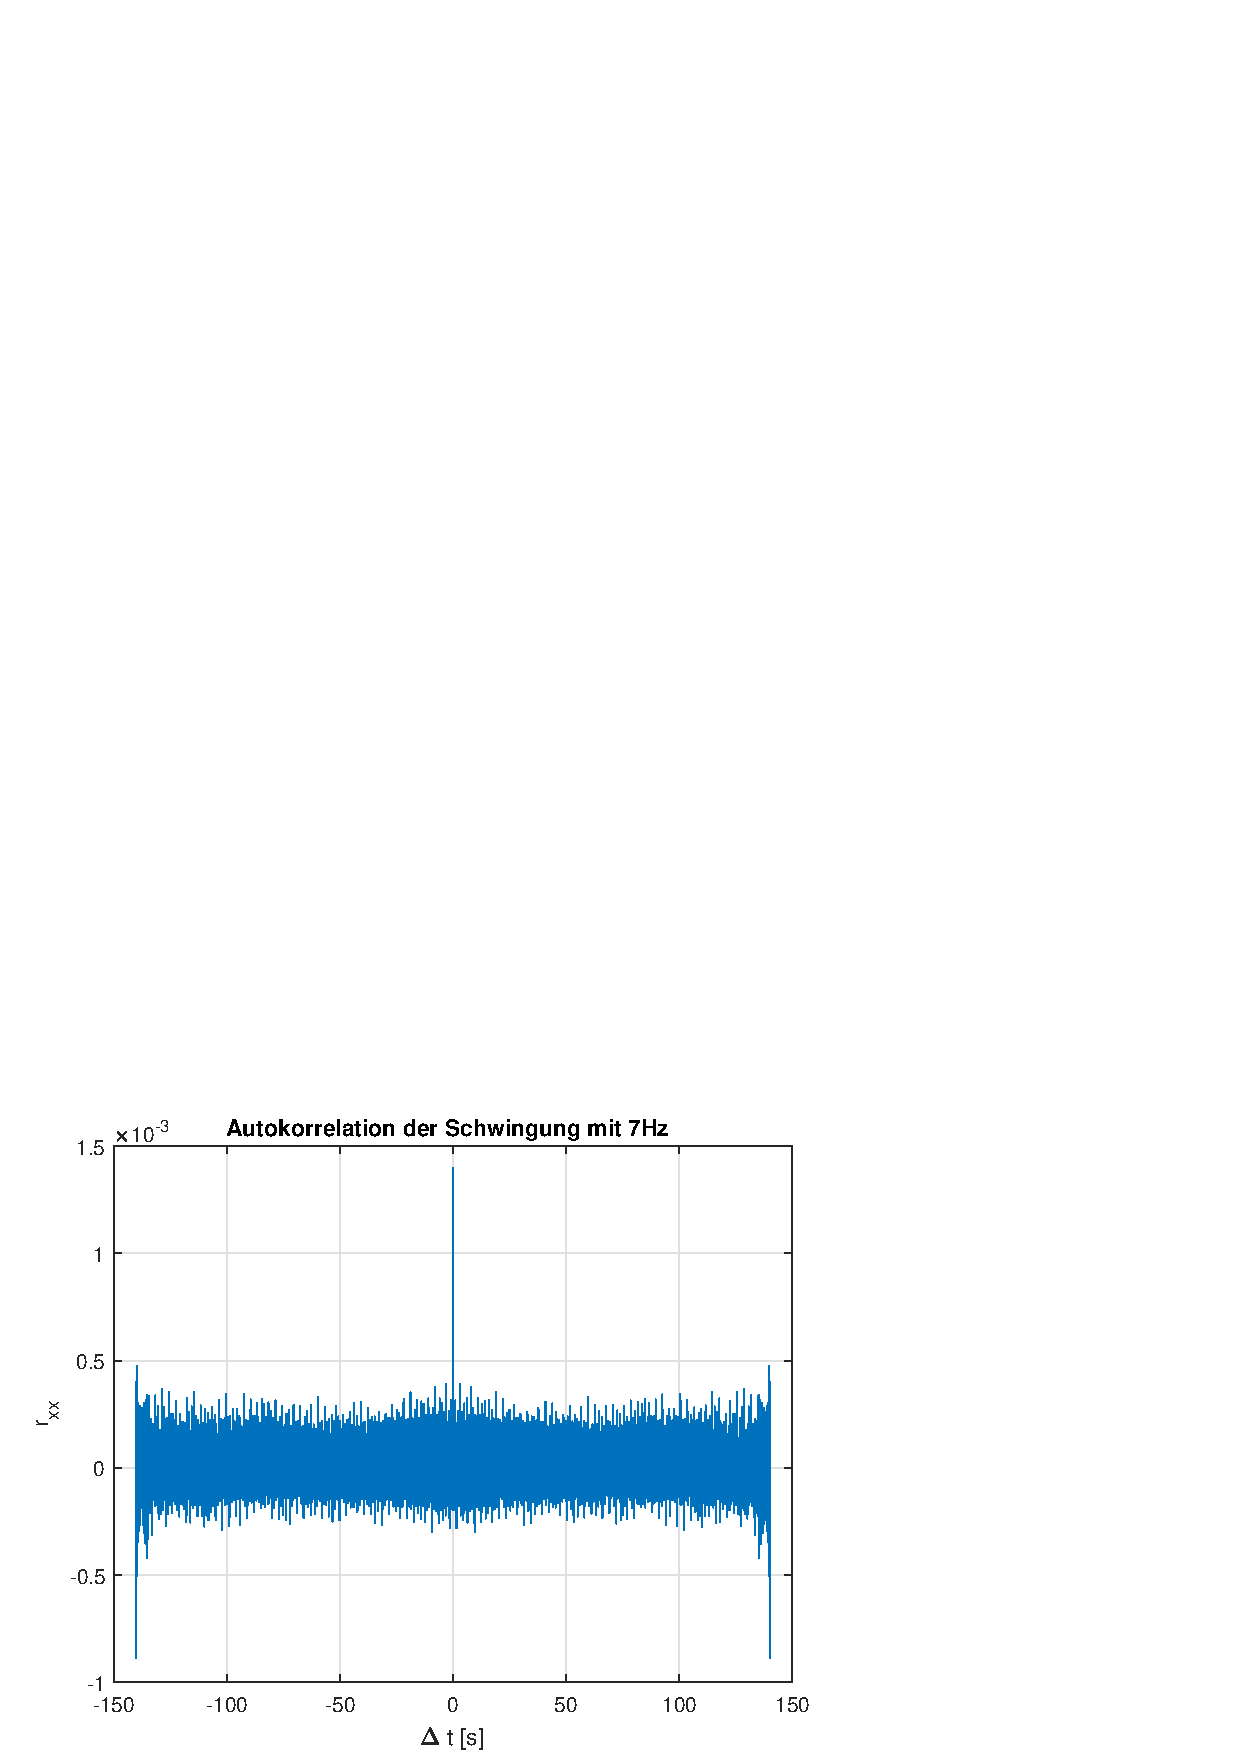
\includegraphics[width=0.5\linewidth]{img/rxx_sinefreq_7}
\end{figure}
\begin{figure}[!h]
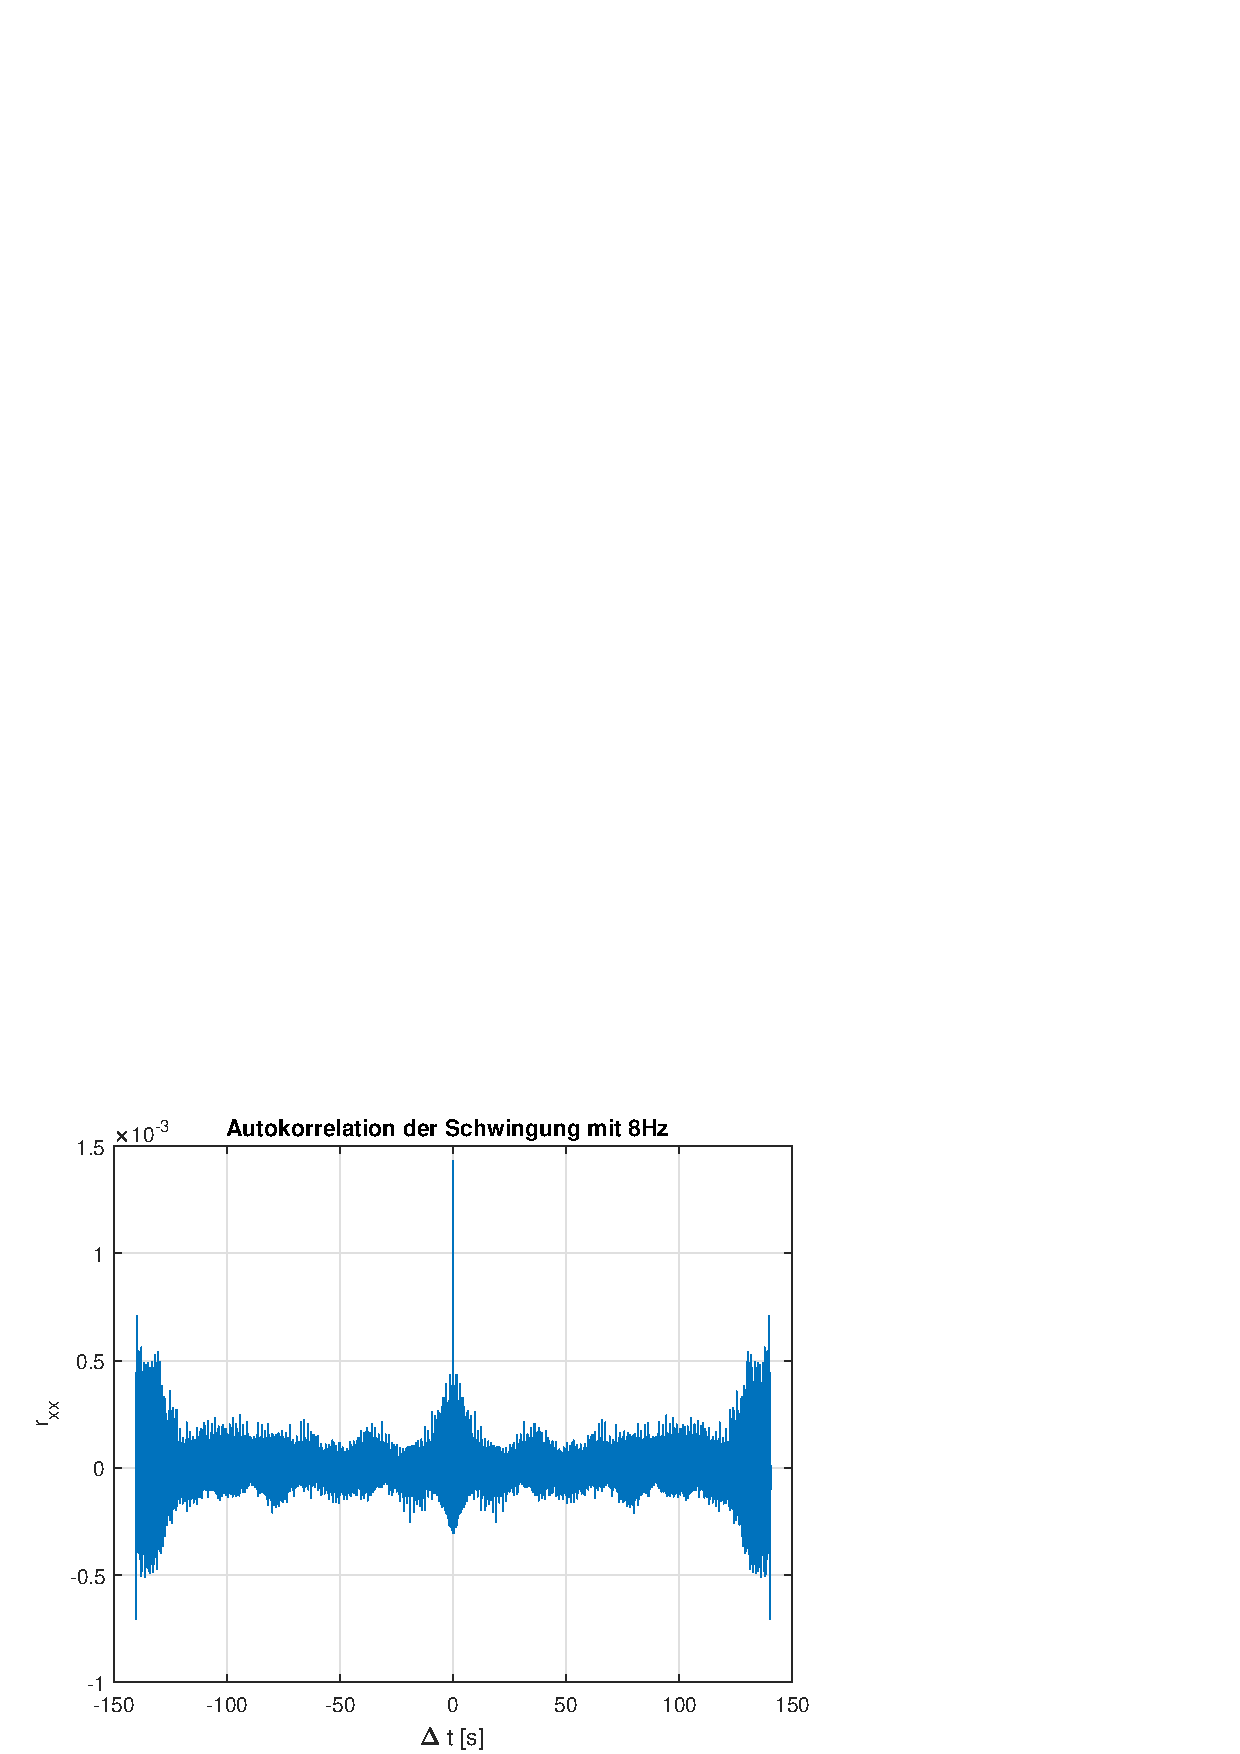
\includegraphics[width=0.5\linewidth]{img/rxx_sinefreq_8}
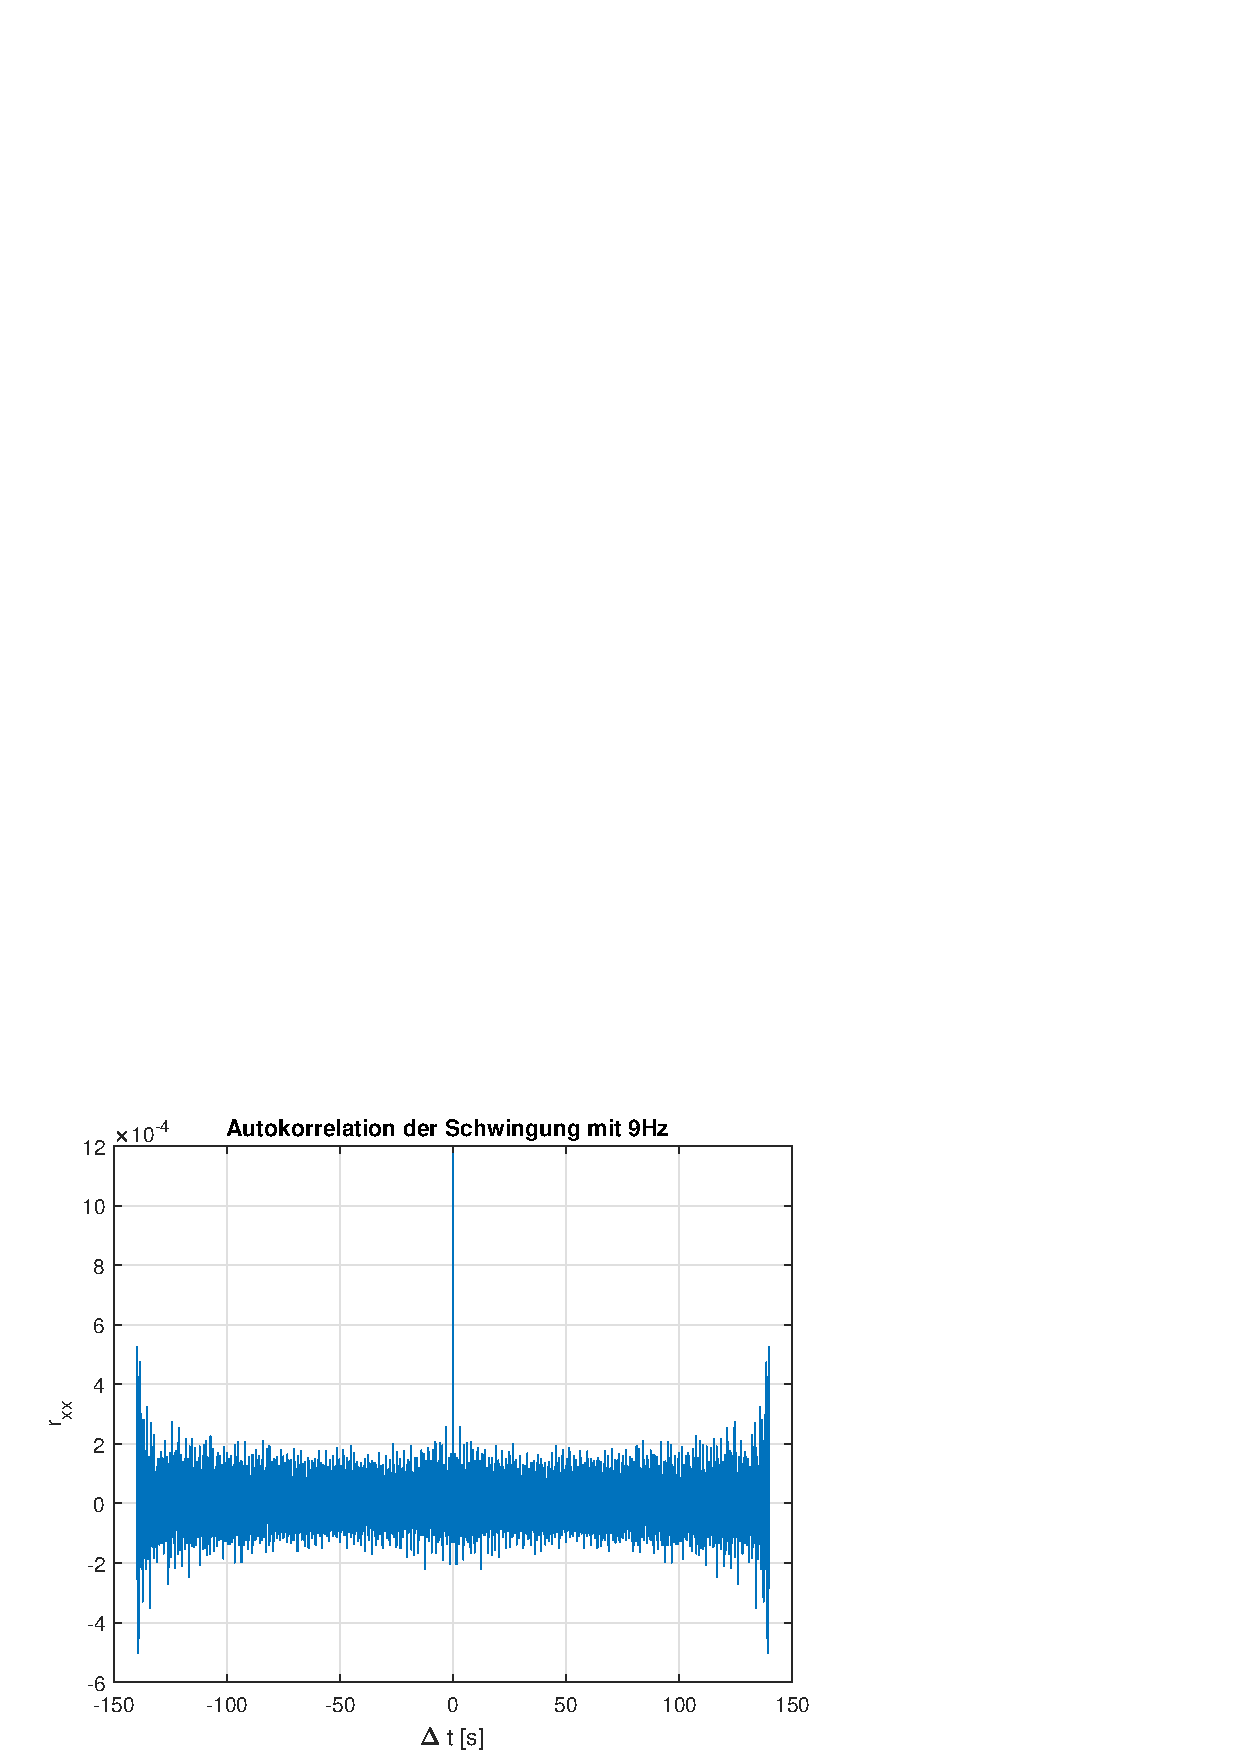
\includegraphics[width=0.5\linewidth]{img/rxx_sinefreq_9}
\end{figure}
\begin{figure}[!h]
\centering
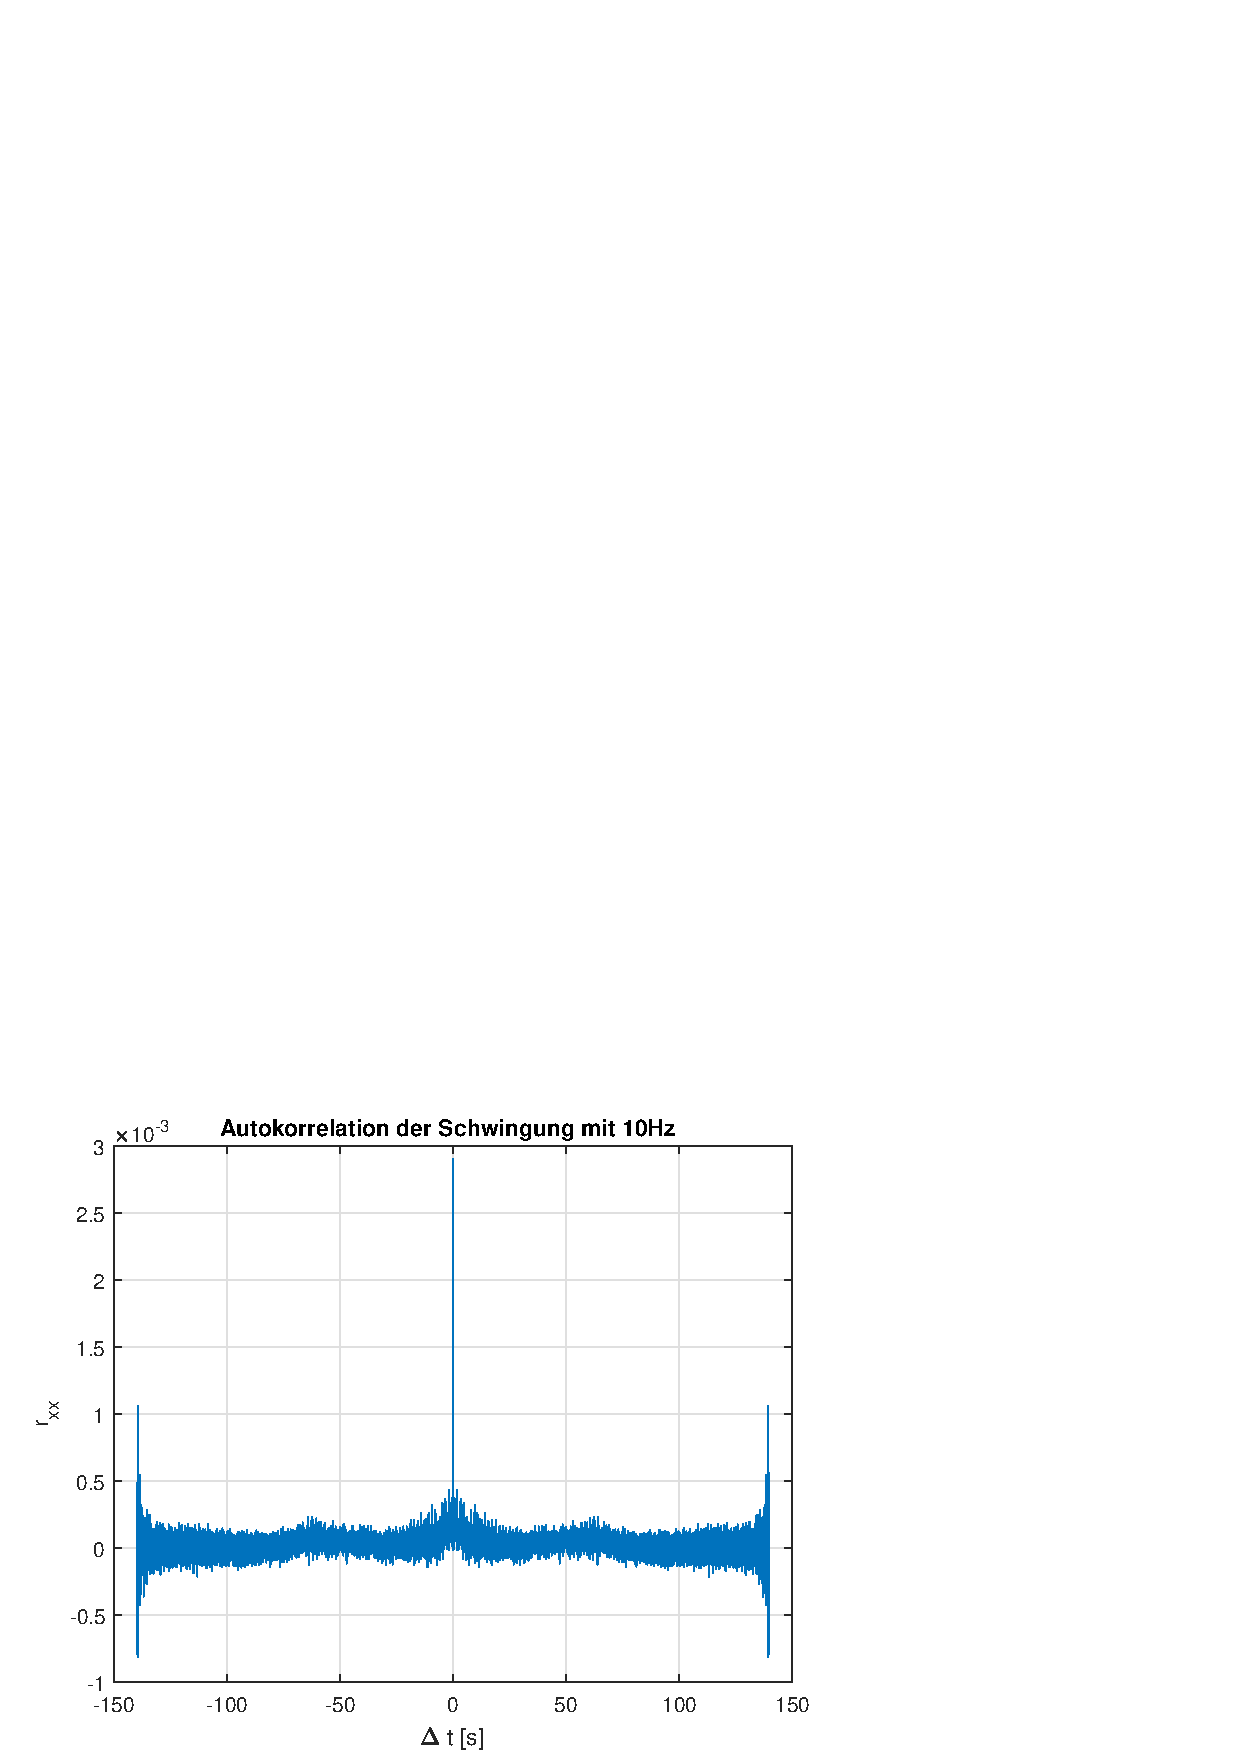
\includegraphics[width=0.5\linewidth]{img/rxx_sinefreq_10}
\end{figure}

\newpage
\subsubsection{Leistungsdichtespektren von $\varphi$ bei $T_M = sin(2\pi\cdot f\cdot t)$}
\begin{figure}[!h]
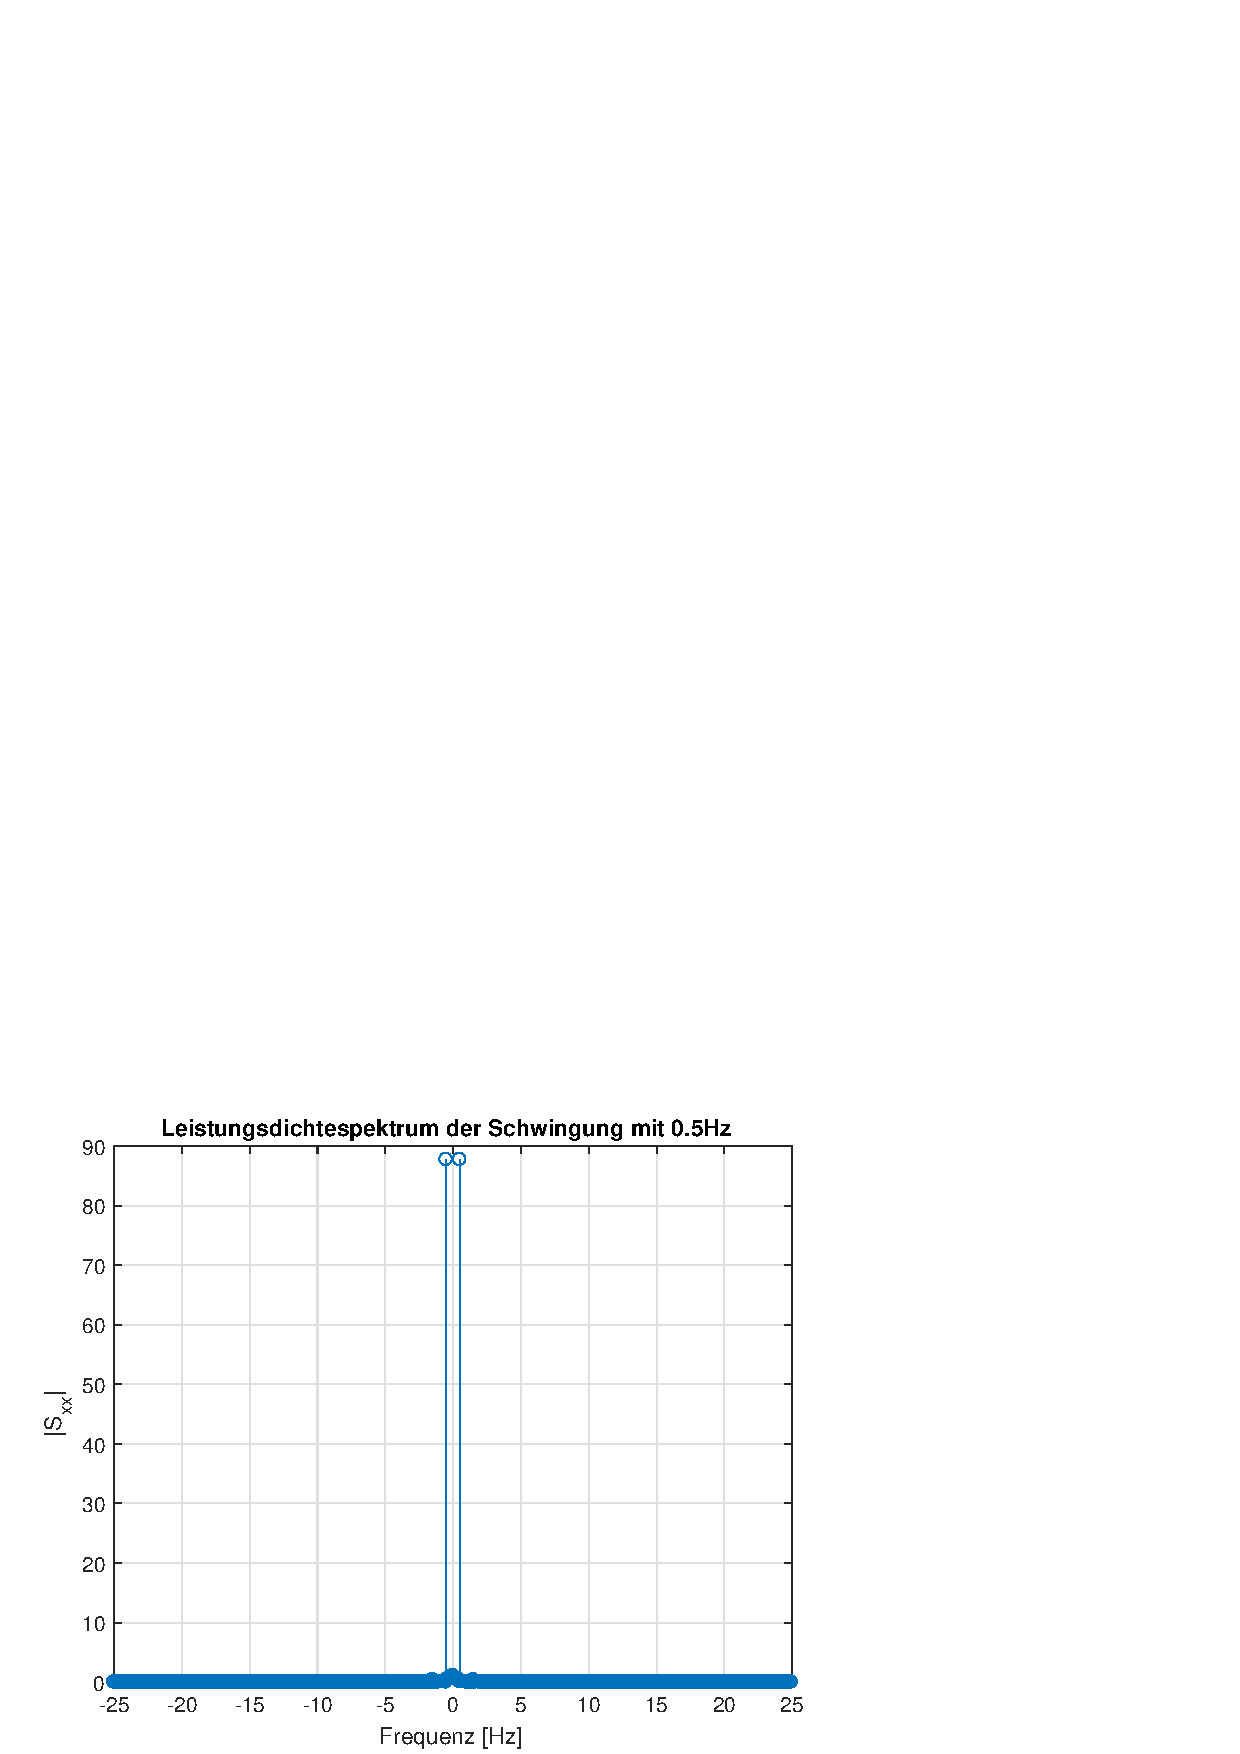
\includegraphics[width=0.5\linewidth]{img/lds_sinefreq_0_5}
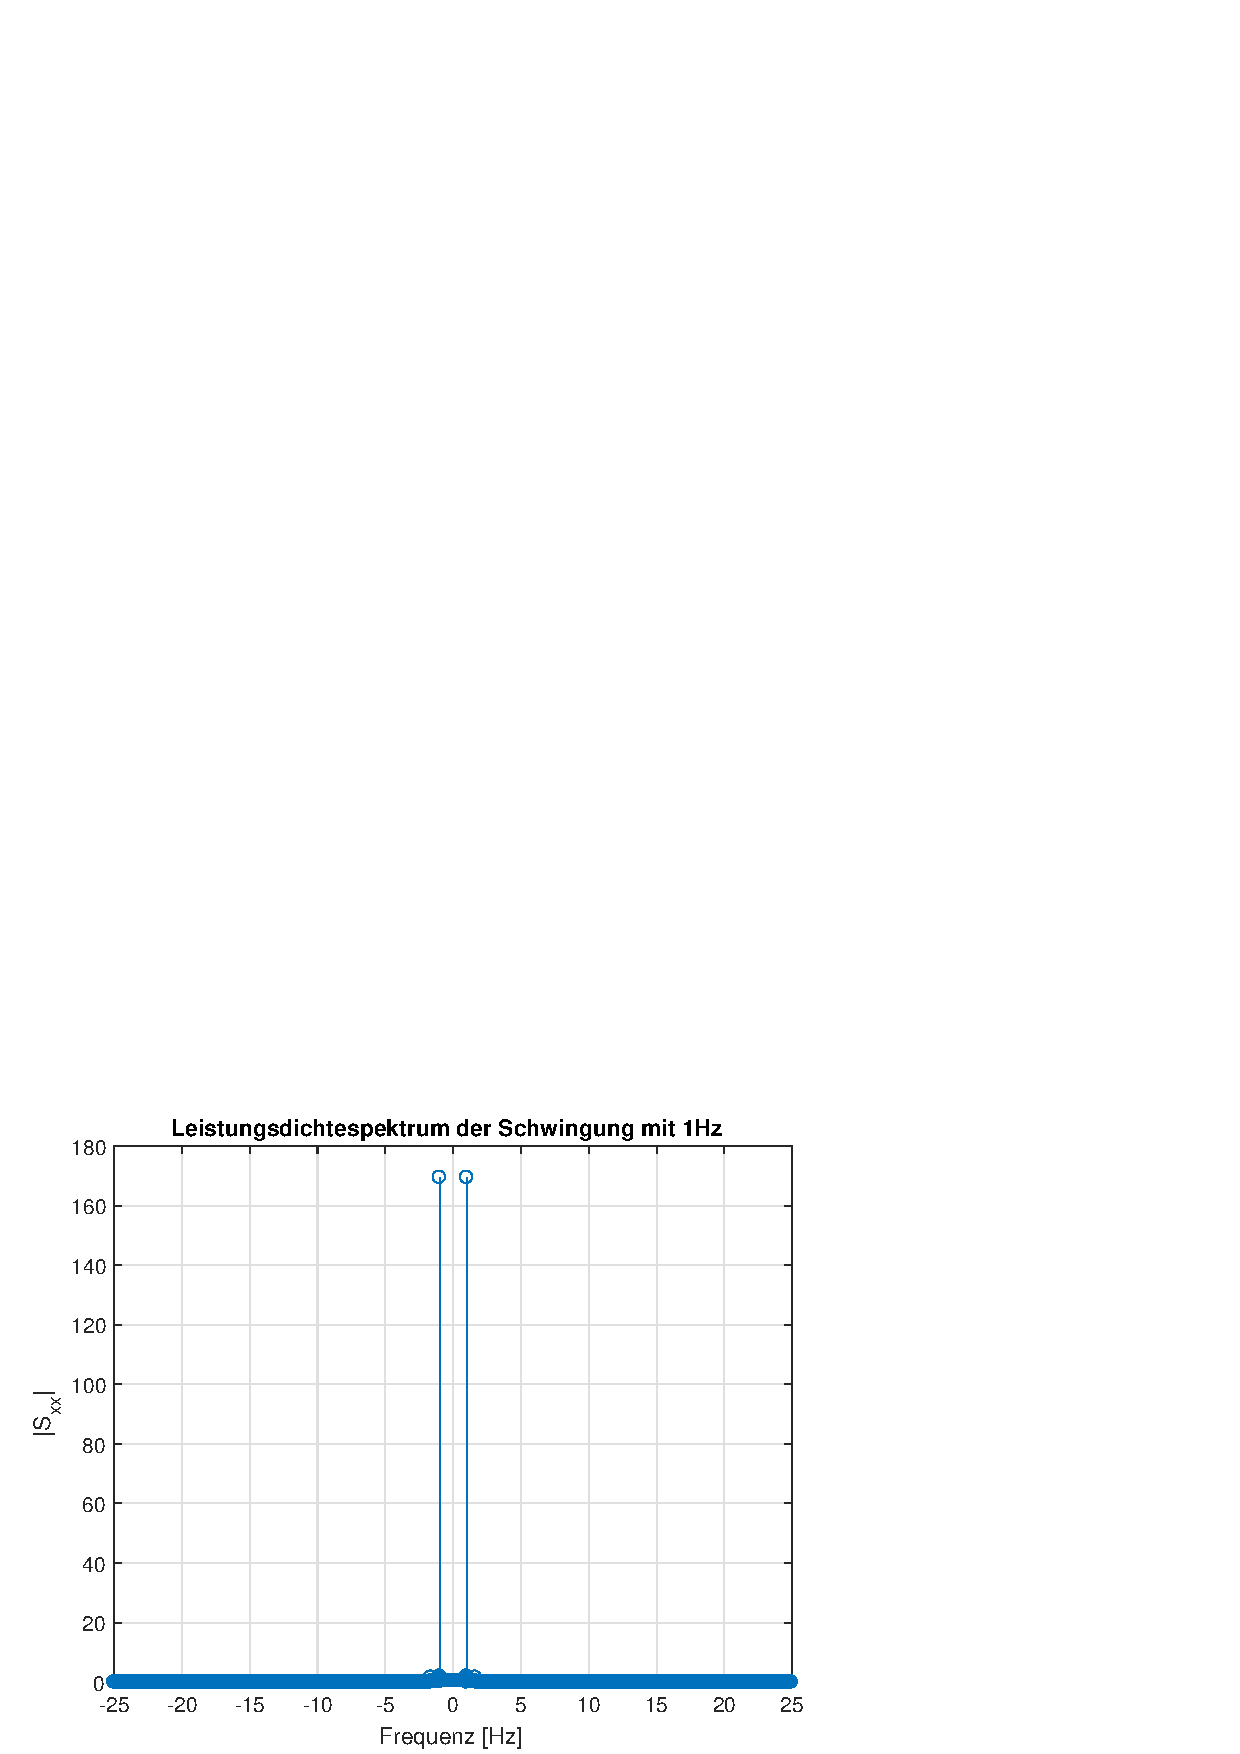
\includegraphics[width=0.5\linewidth]{img/lds_sinefreq_1}
\end{figure}
\begin{figure}[!h]
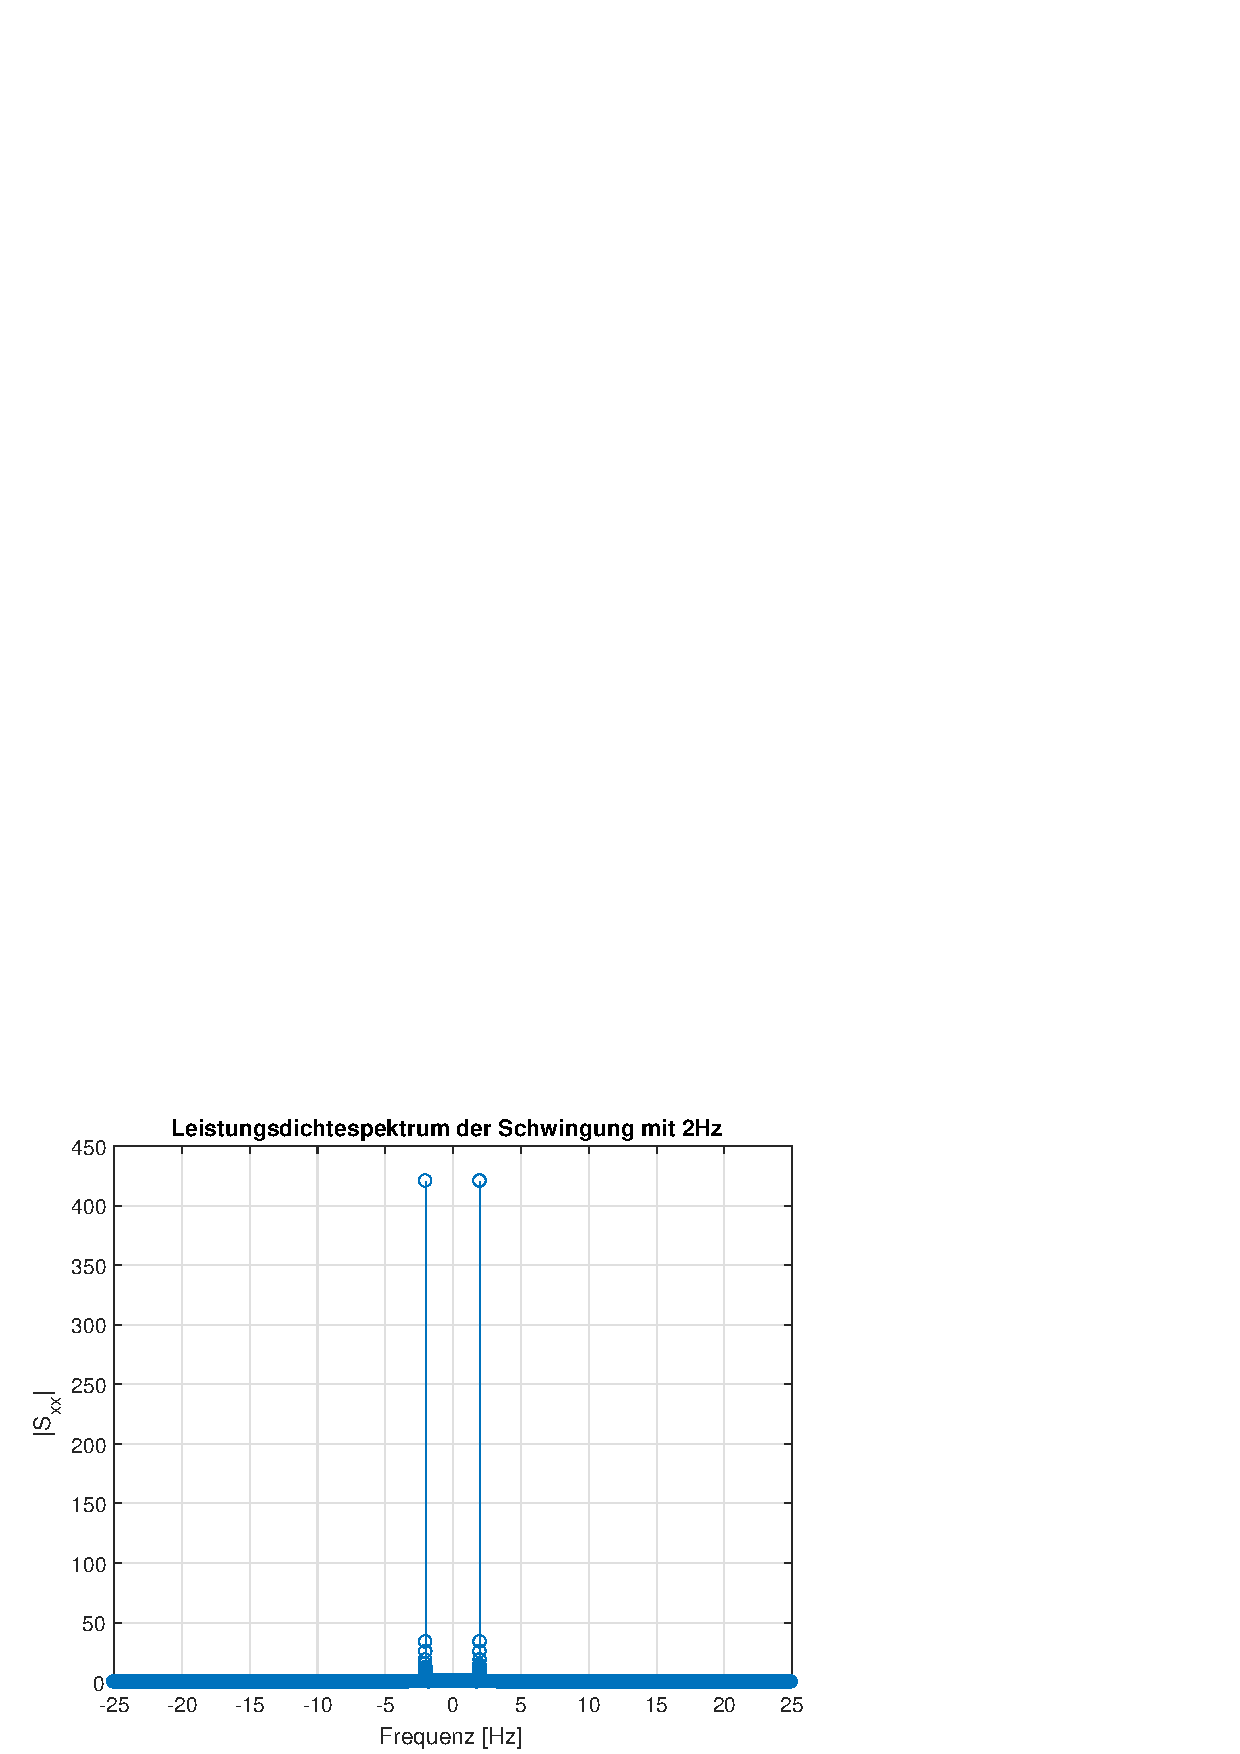
\includegraphics[width=0.5\linewidth]{img/lds_sinefreq_2}
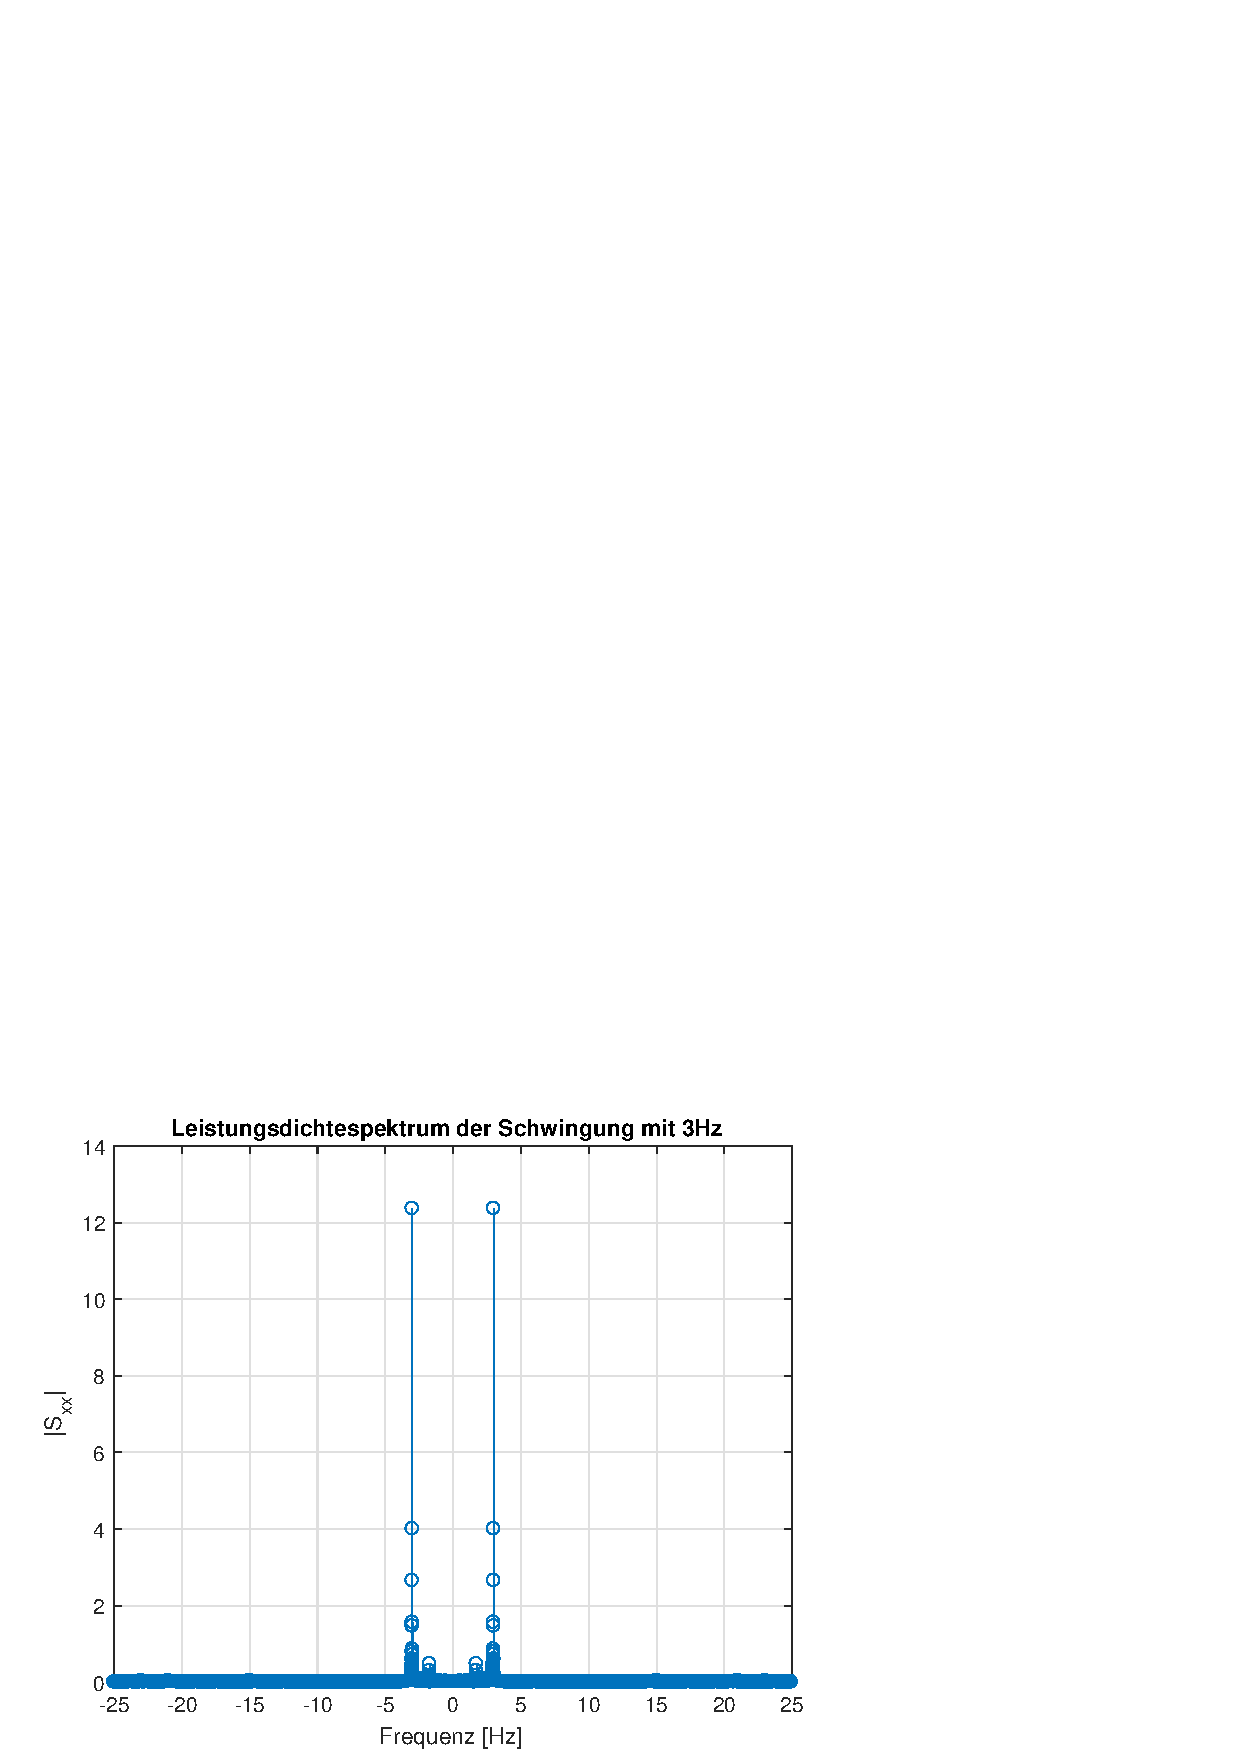
\includegraphics[width=0.5\linewidth]{img/lds_sinefreq_3}
\end{figure}
\begin{figure}[!h]
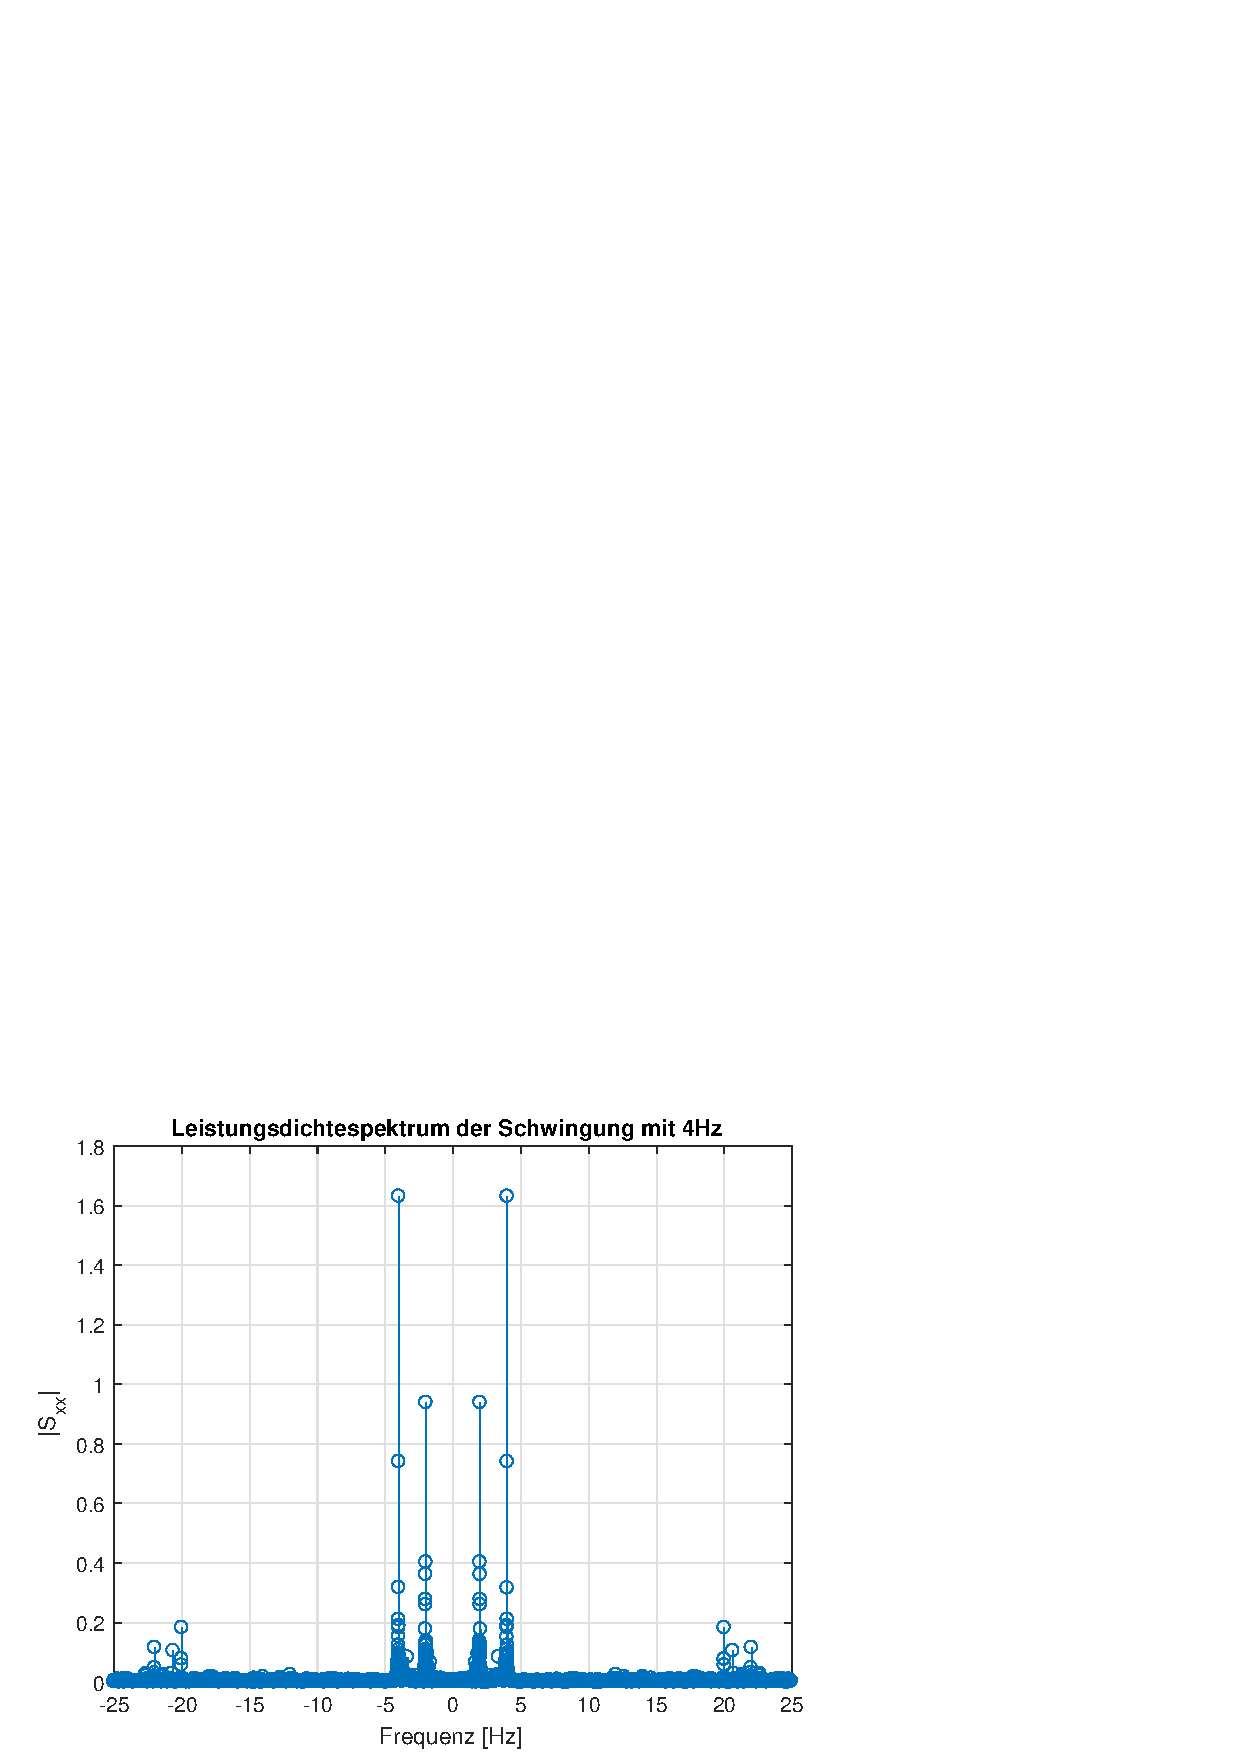
\includegraphics[width=0.5\linewidth]{img/lds_sinefreq_4}
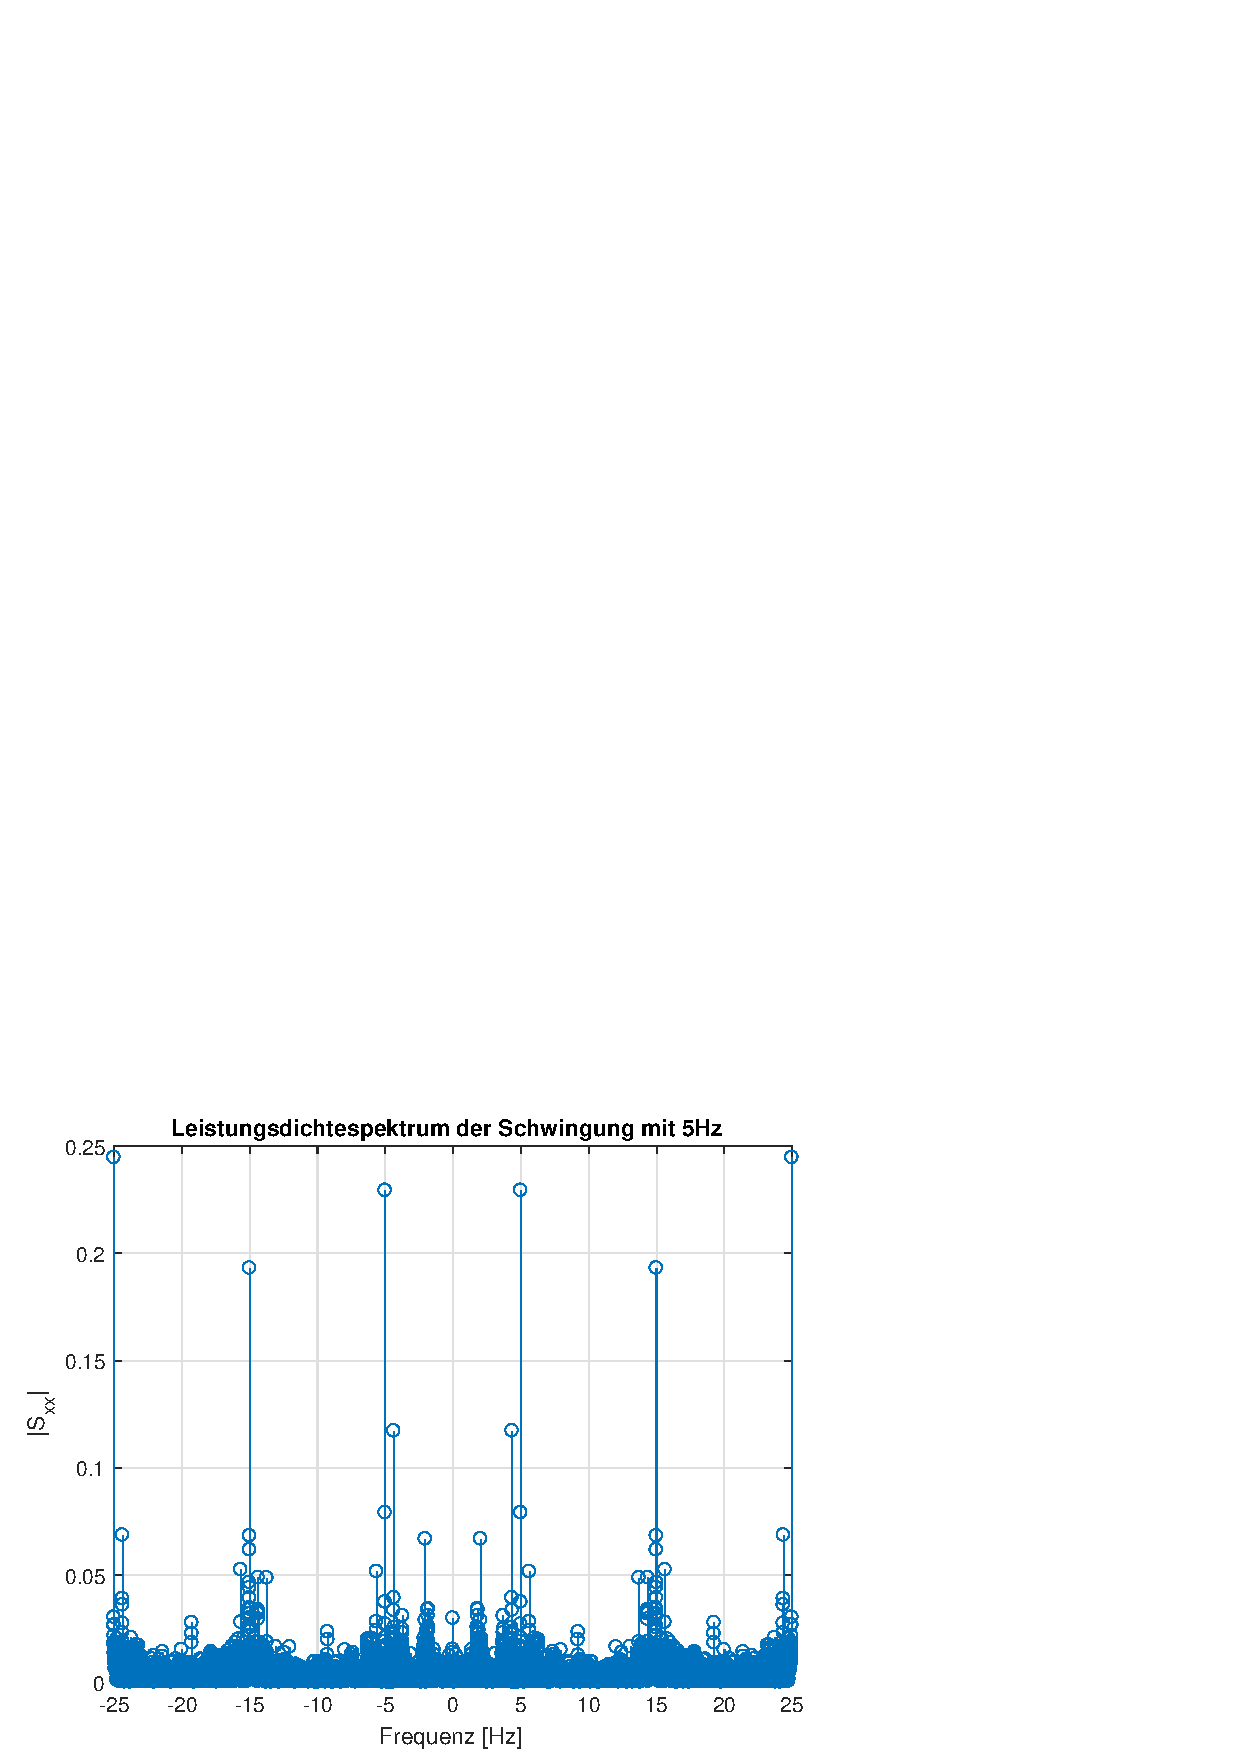
\includegraphics[width=0.5\linewidth]{img/lds_sinefreq_5}
\end{figure}
\begin{figure}[!h]
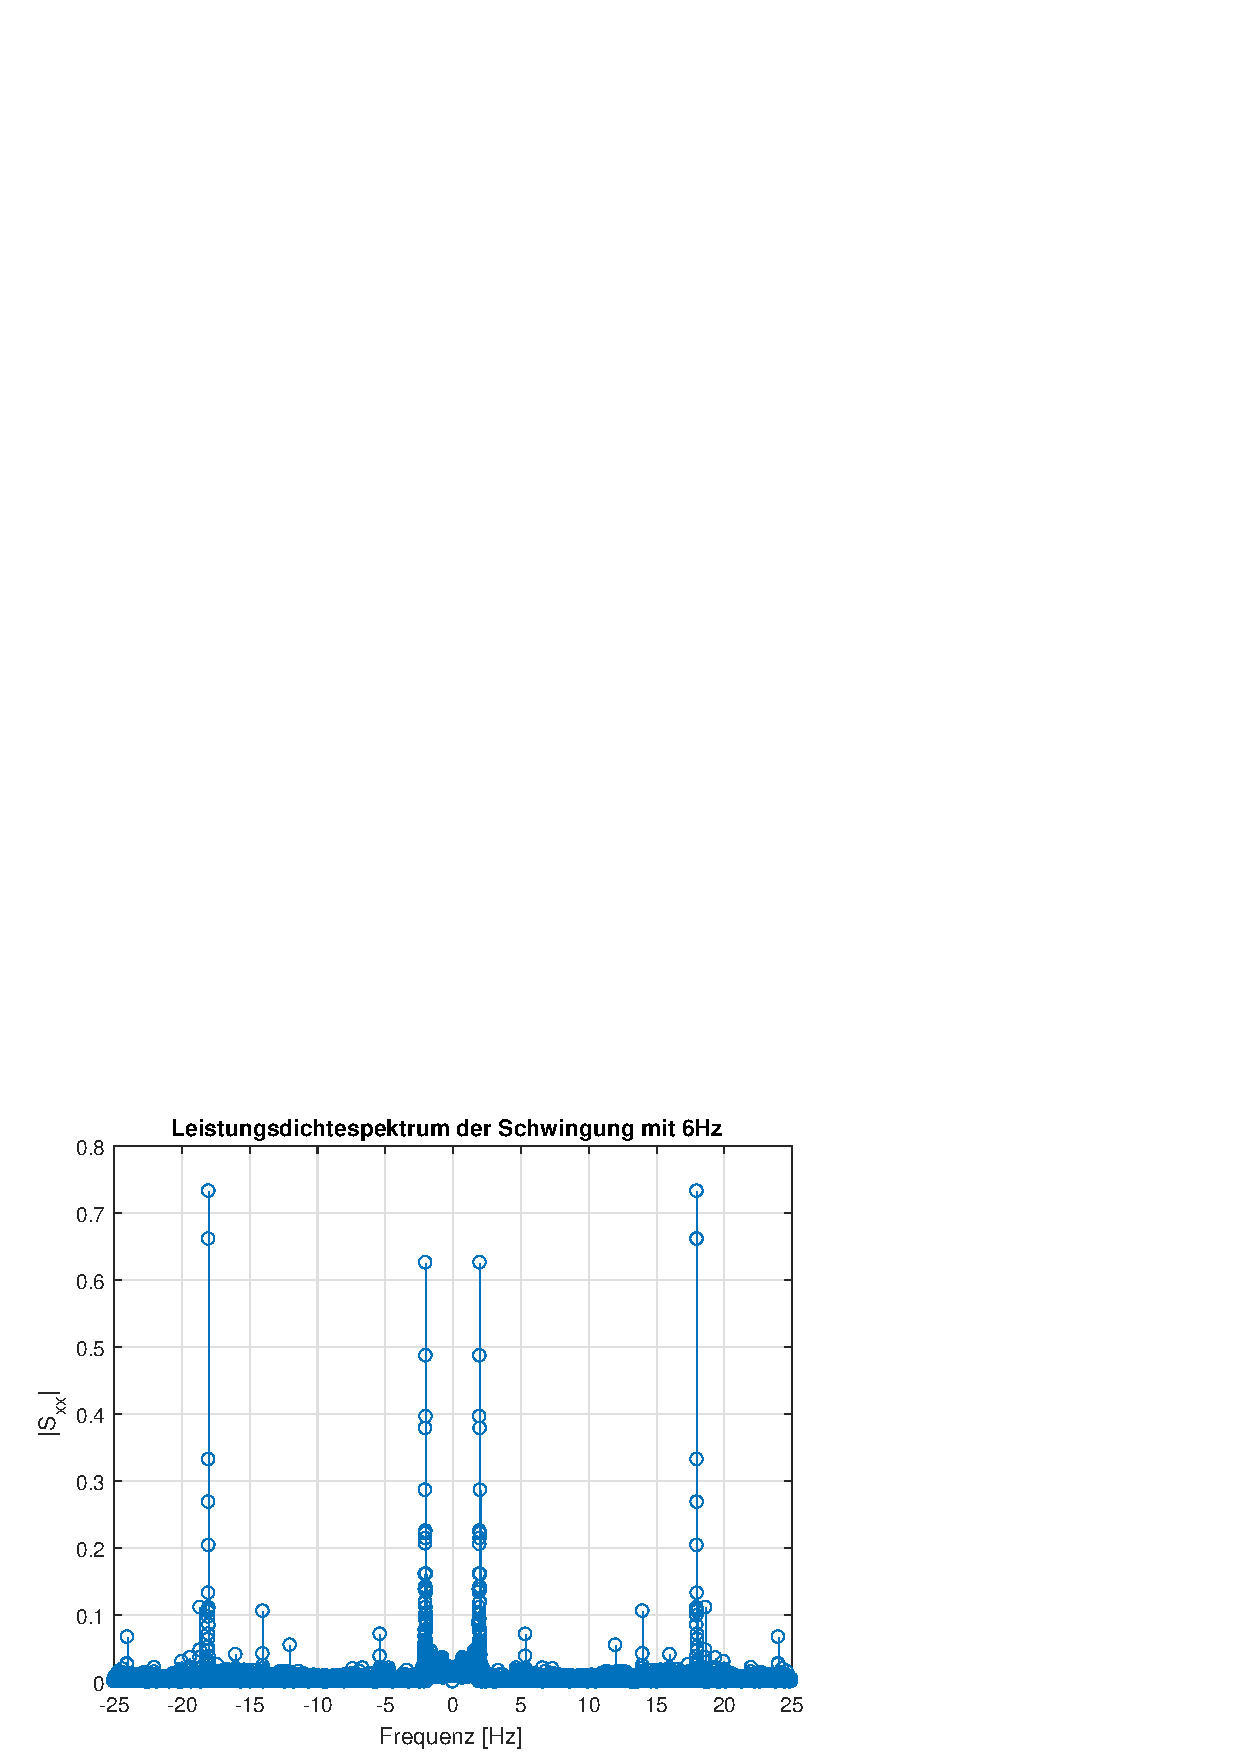
\includegraphics[width=0.5\linewidth]{img/lds_sinefreq_6}
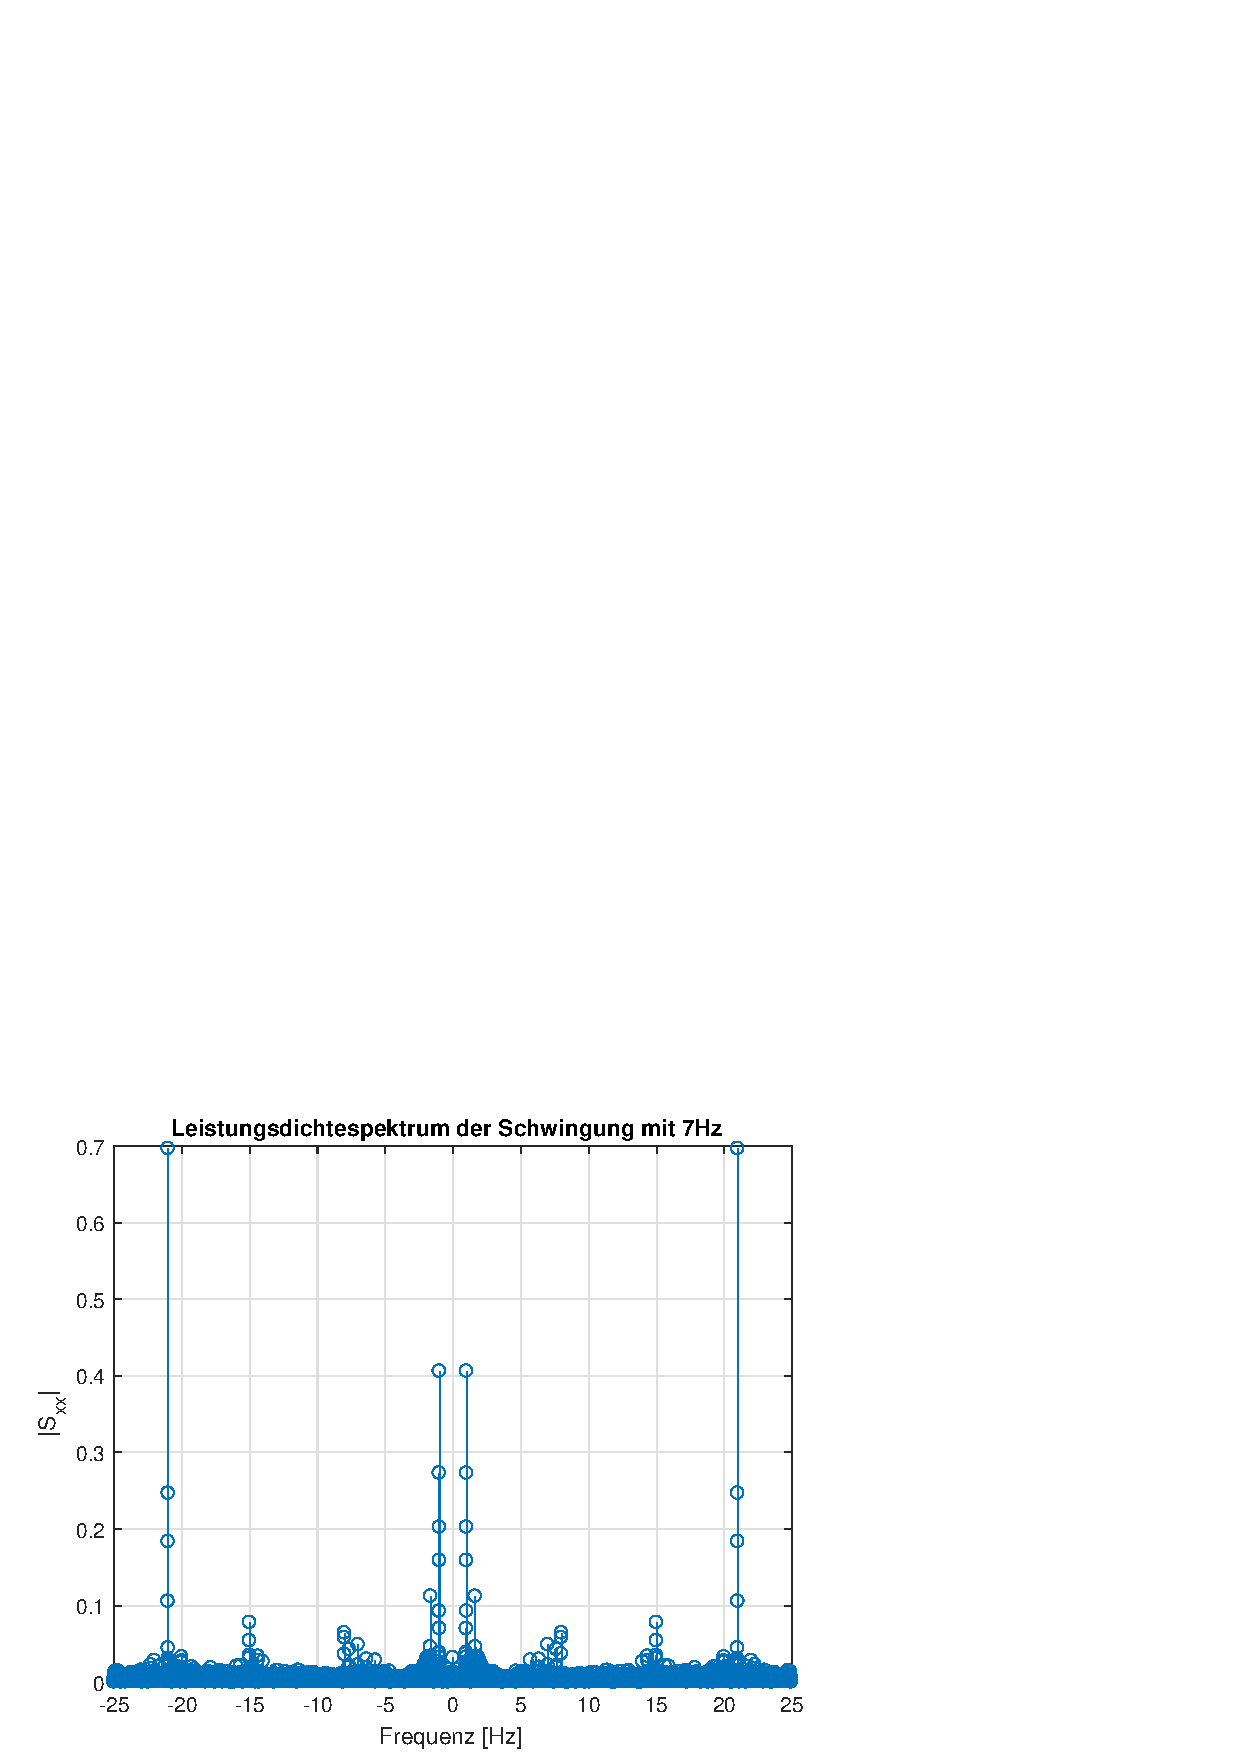
\includegraphics[width=0.5\linewidth]{img/lds_sinefreq_7}
\end{figure}
\begin{figure}[!h]
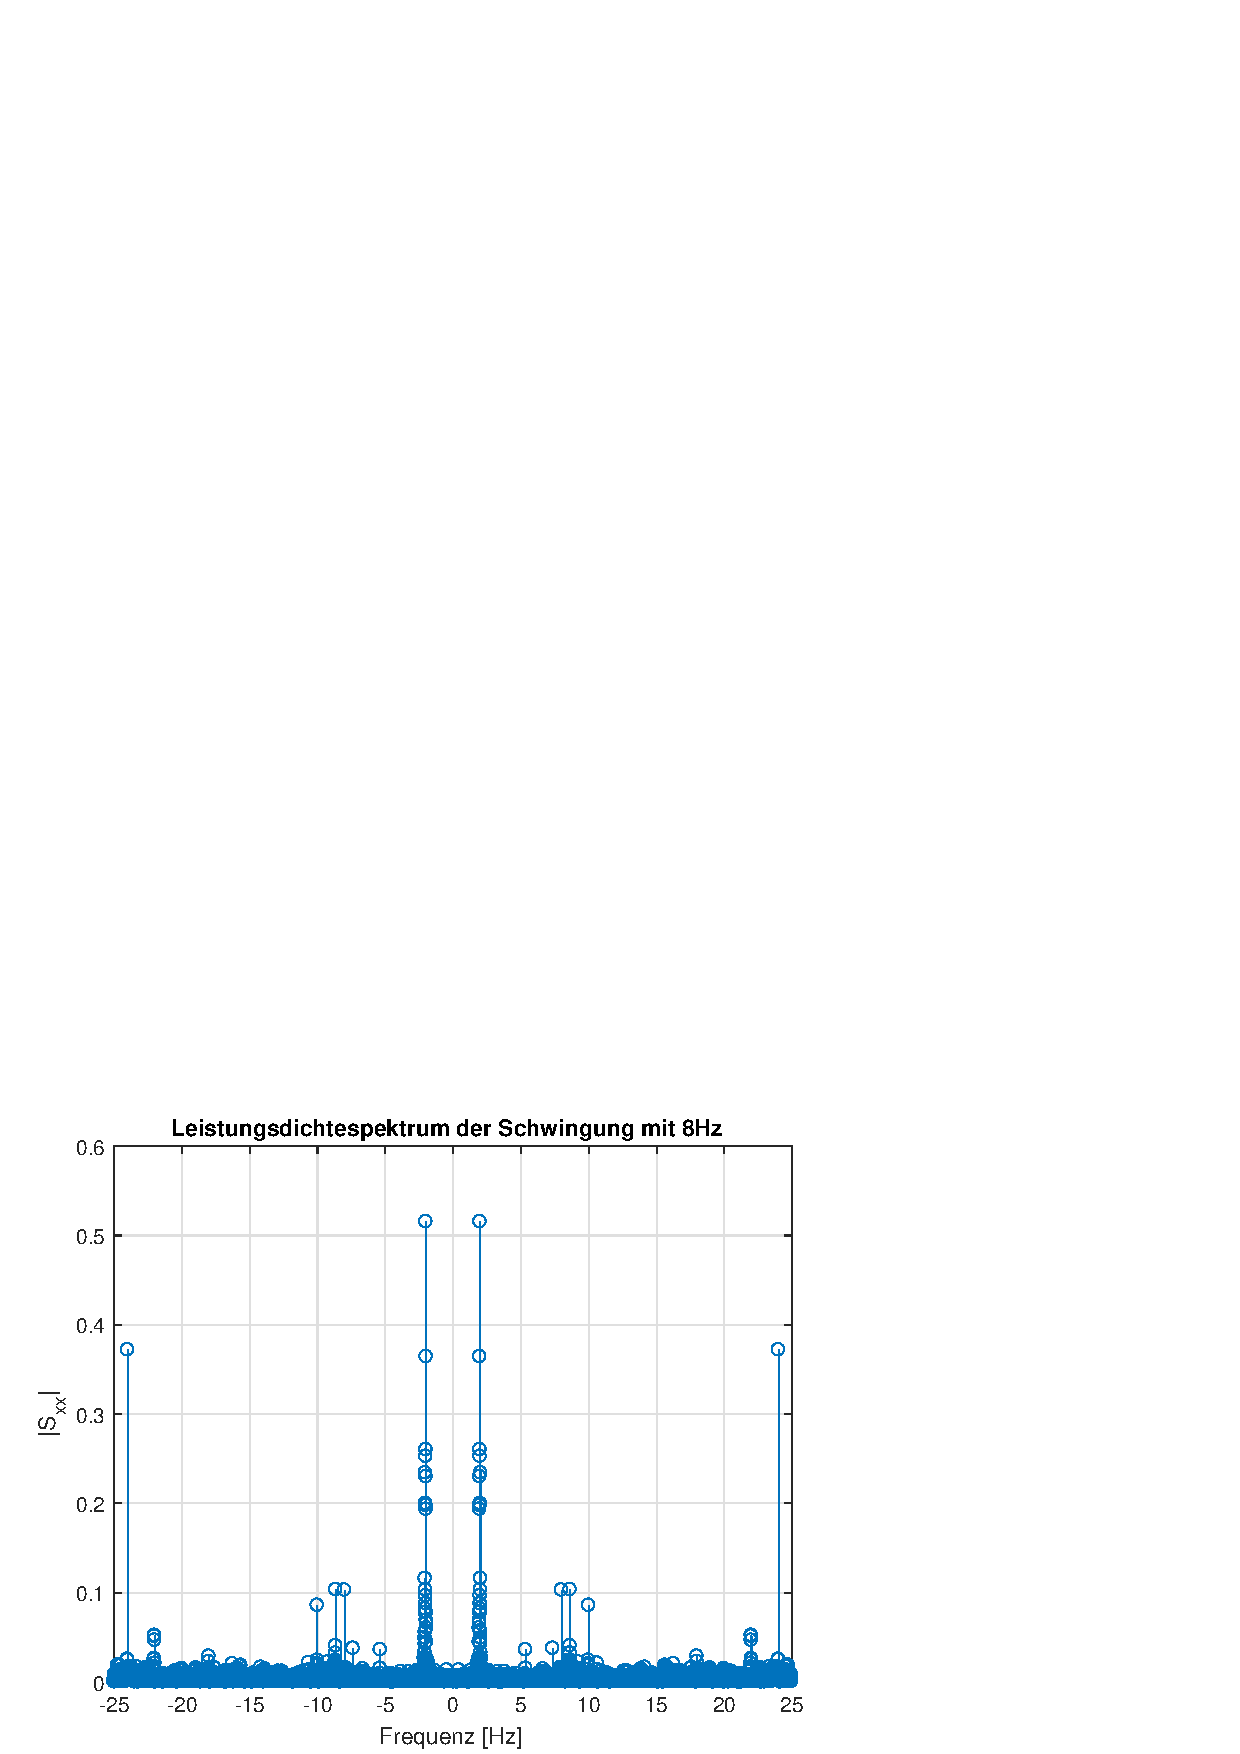
\includegraphics[width=0.5\linewidth]{img/lds_sinefreq_8}
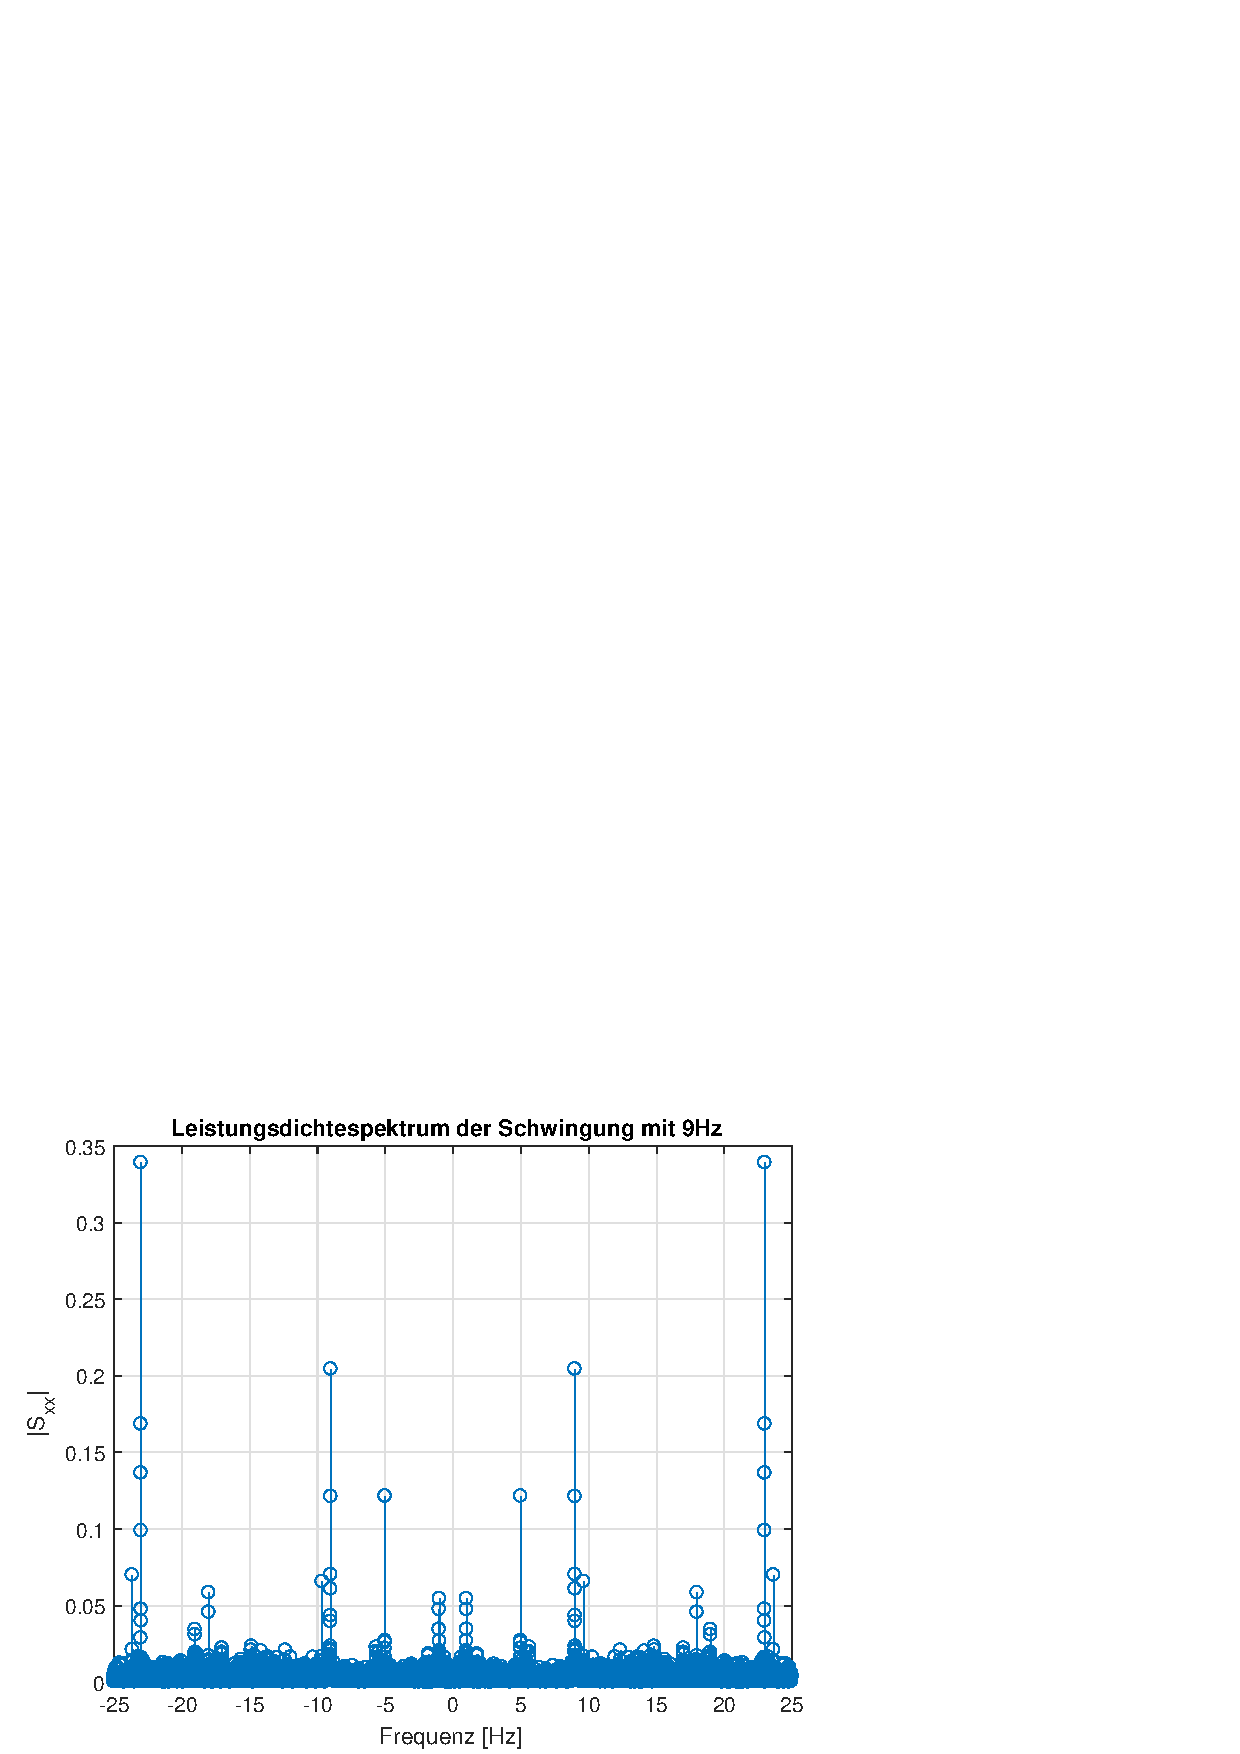
\includegraphics[width=0.5\linewidth]{img/lds_sinefreq_9}
\end{figure}
\begin{figure}[!h]
\centering
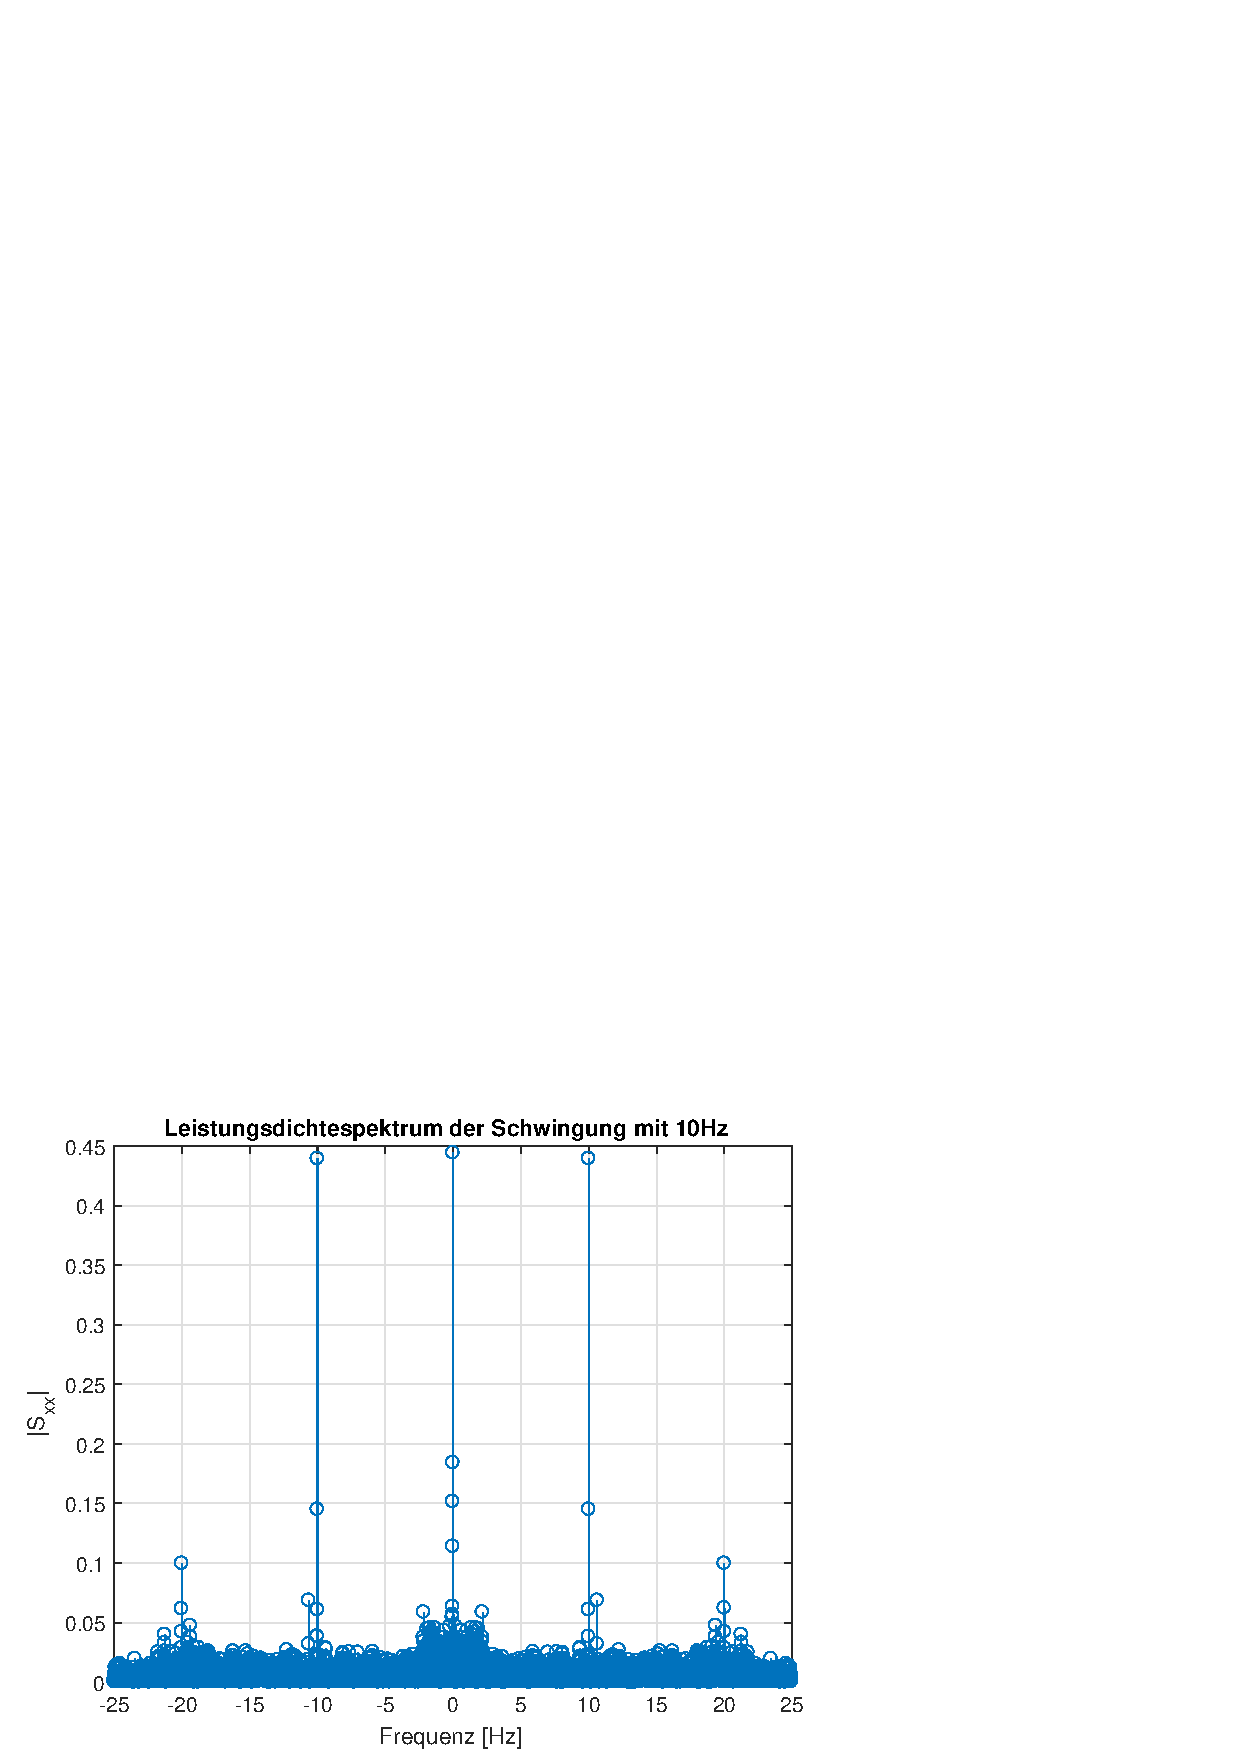
\includegraphics[width=0.5\linewidth]{img/lds_sinefreq_10}
\end{figure}


\newpage
\subsection{Simulationplots $varphi$}
\subsubsection{Verlauf von $\varphi$ bei $T_M = sin(2\pi\cdot f \cdot t)$}
\begin{figure}[!h]
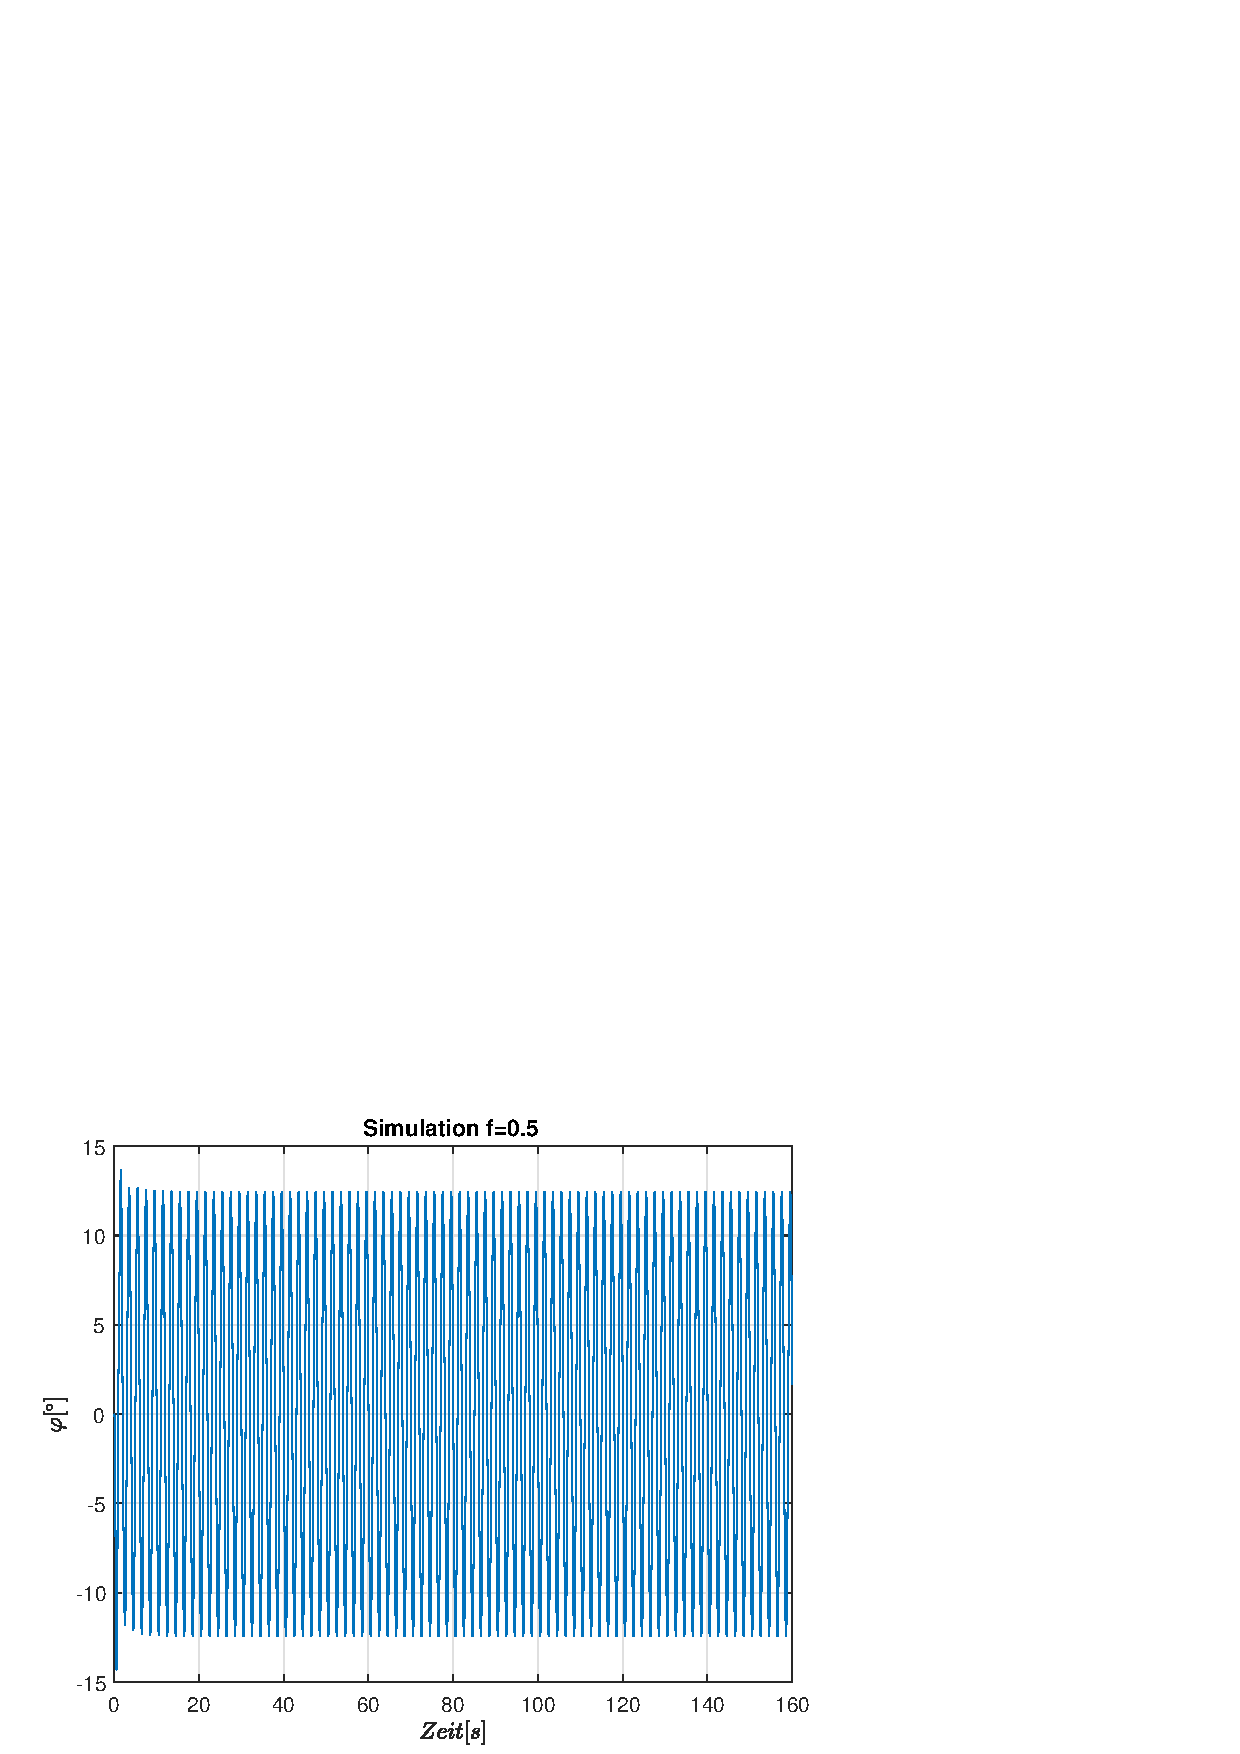
\includegraphics[width=0.5\linewidth]{img/sim_phi_sine_freq_0_5}
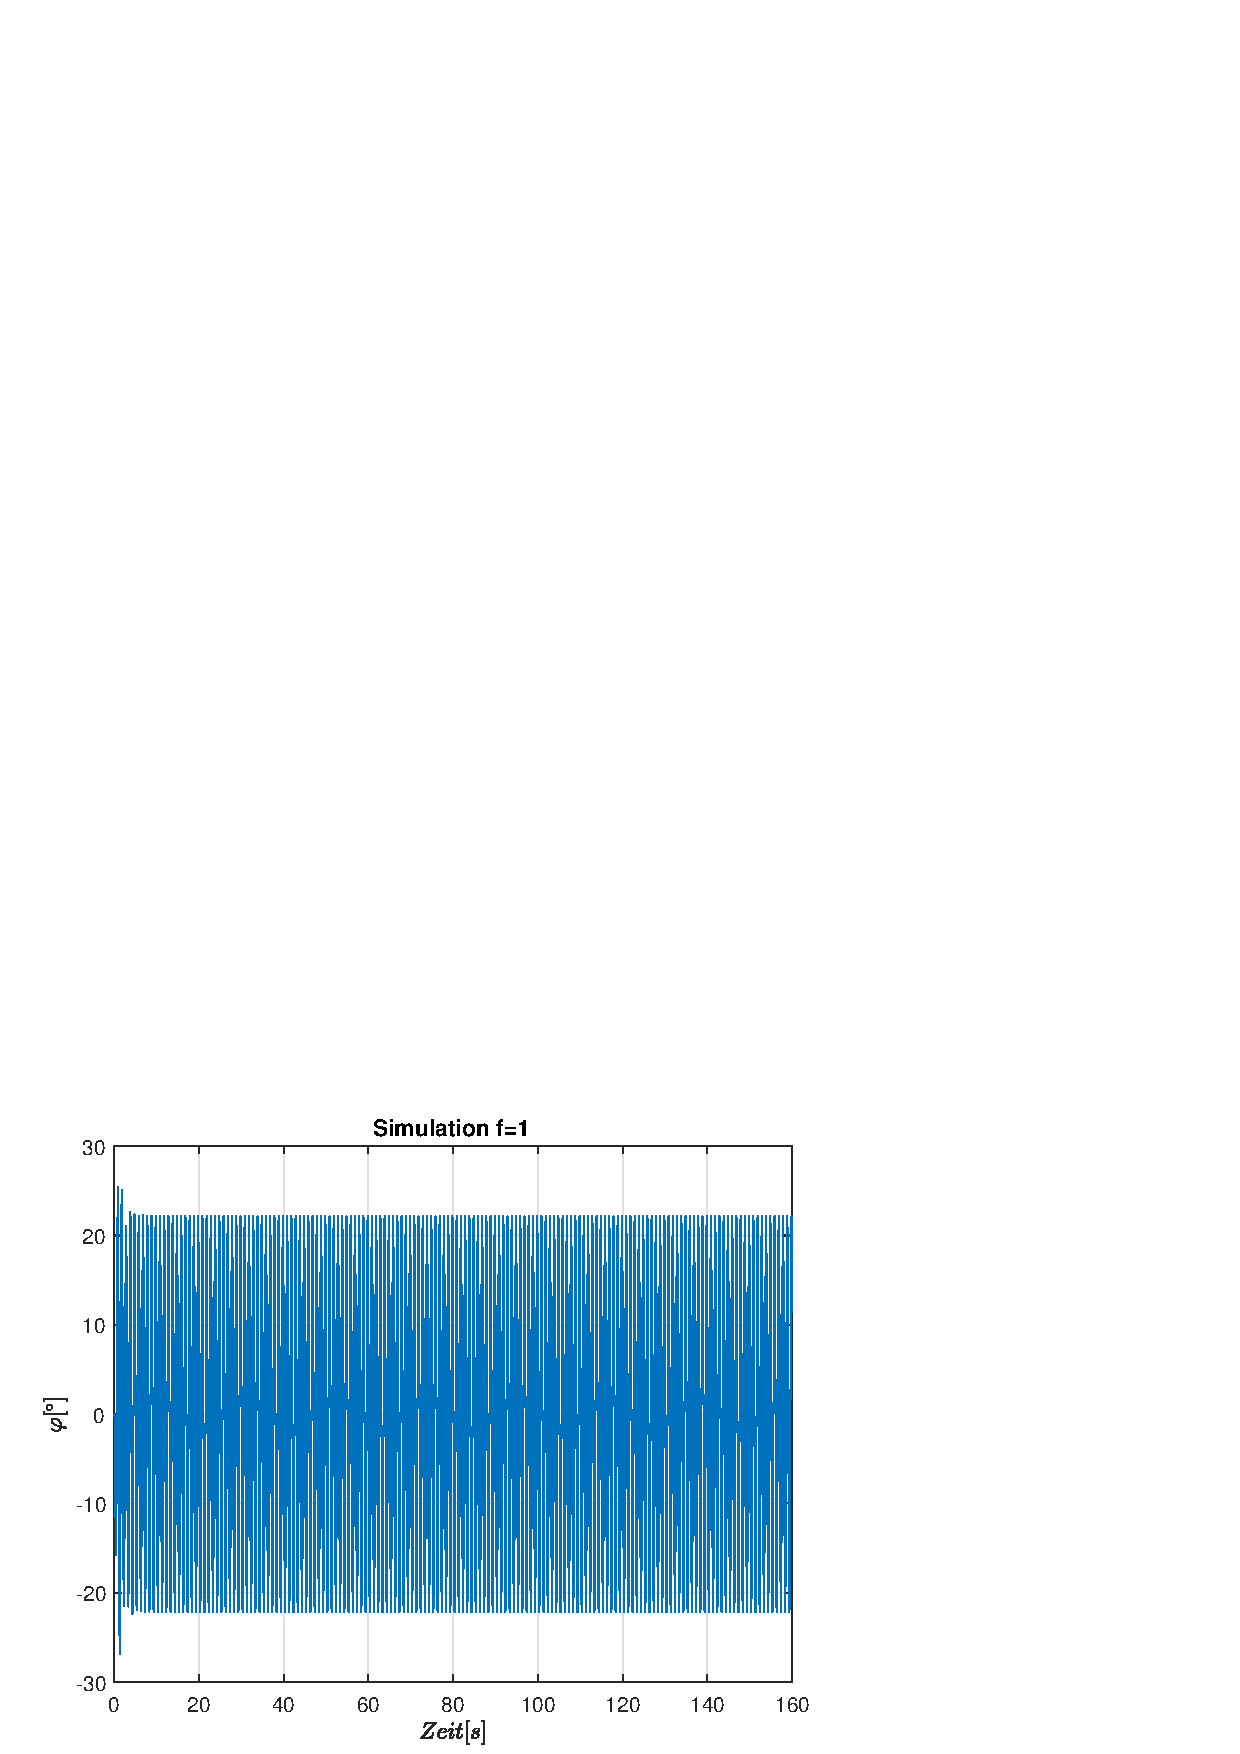
\includegraphics[width=0.5\linewidth]{img/sim_phi_sine_freq_1}
\end{figure}
\begin{figure}[!h]
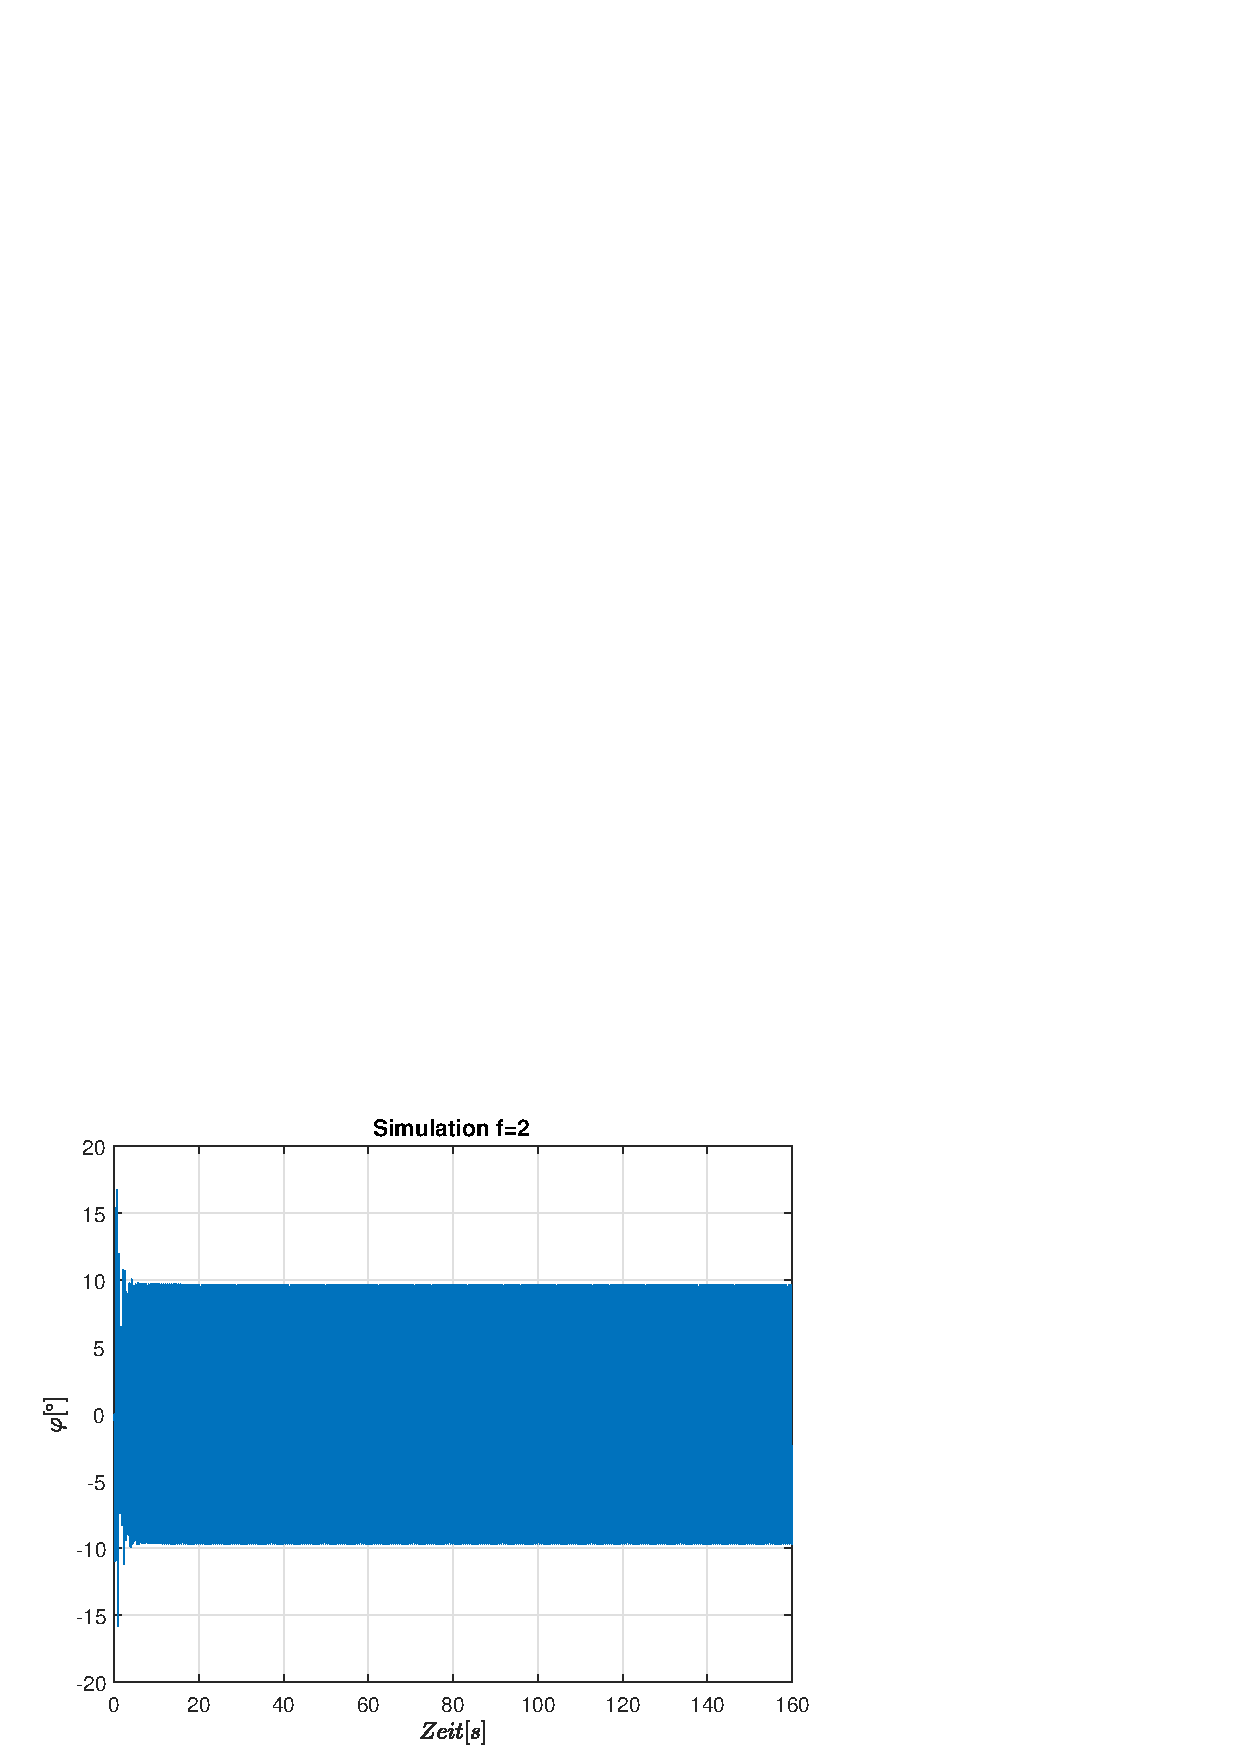
\includegraphics[width=0.5\linewidth]{img/sim_phi_sine_freq_2}
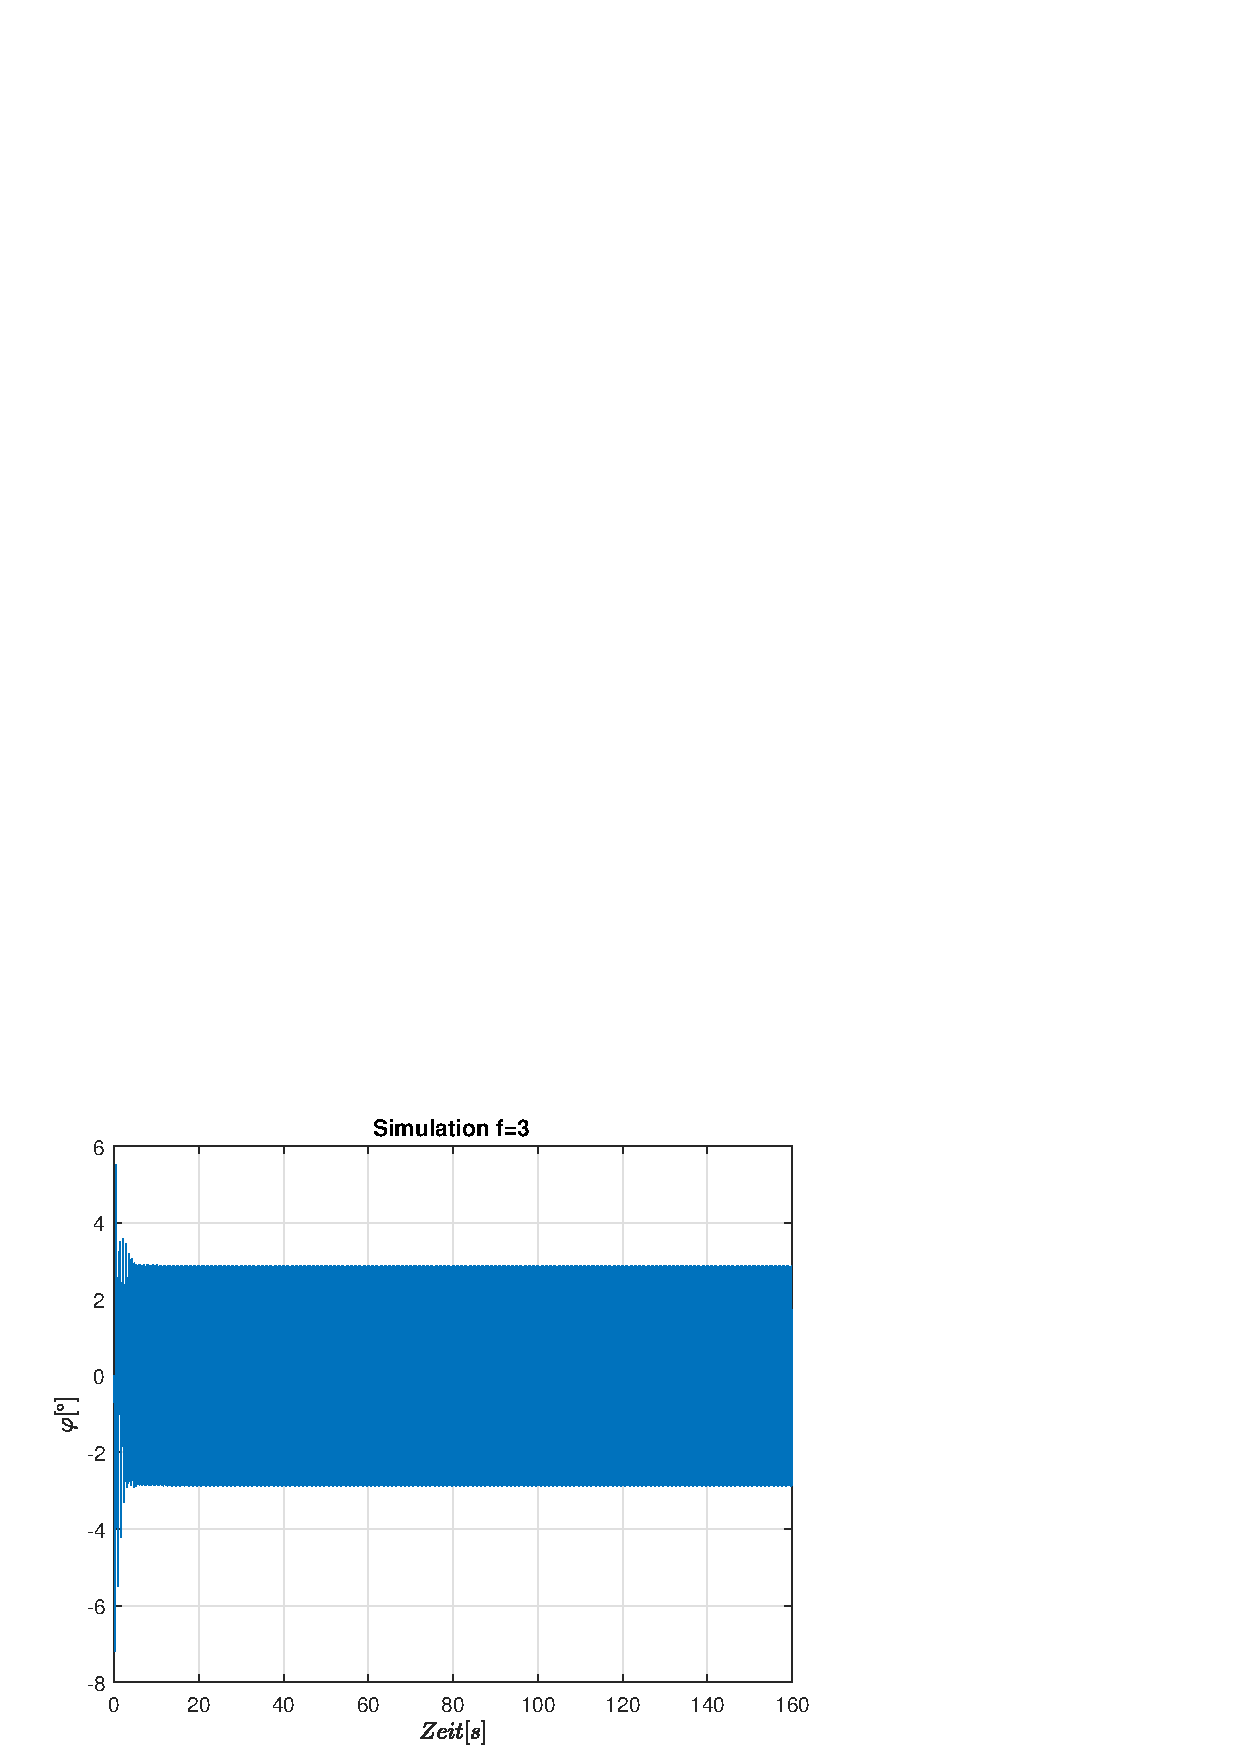
\includegraphics[width=0.5\linewidth]{img/sim_phi_sine_freq_3}
\end{figure}
\begin{figure}[!h]
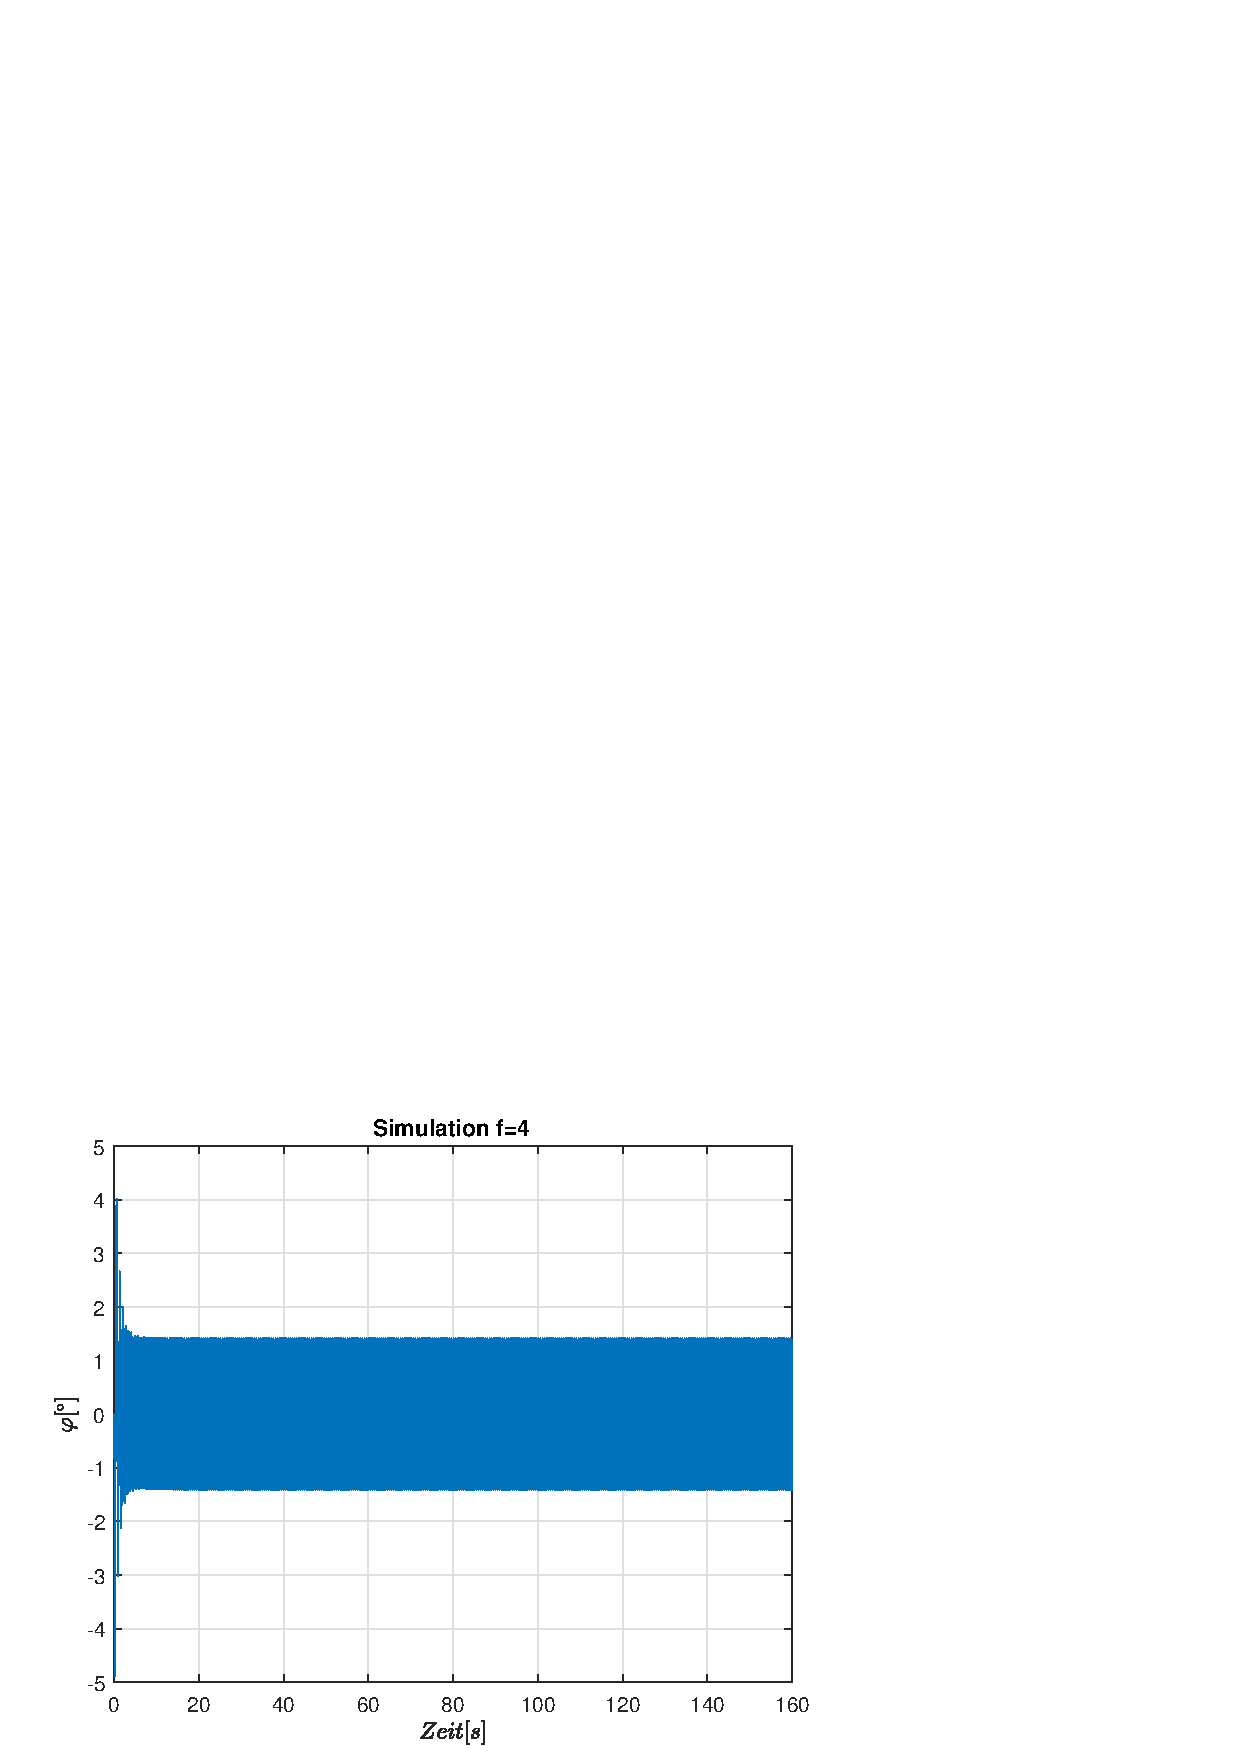
\includegraphics[width=0.5\linewidth]{img/sim_phi_sine_freq_4}
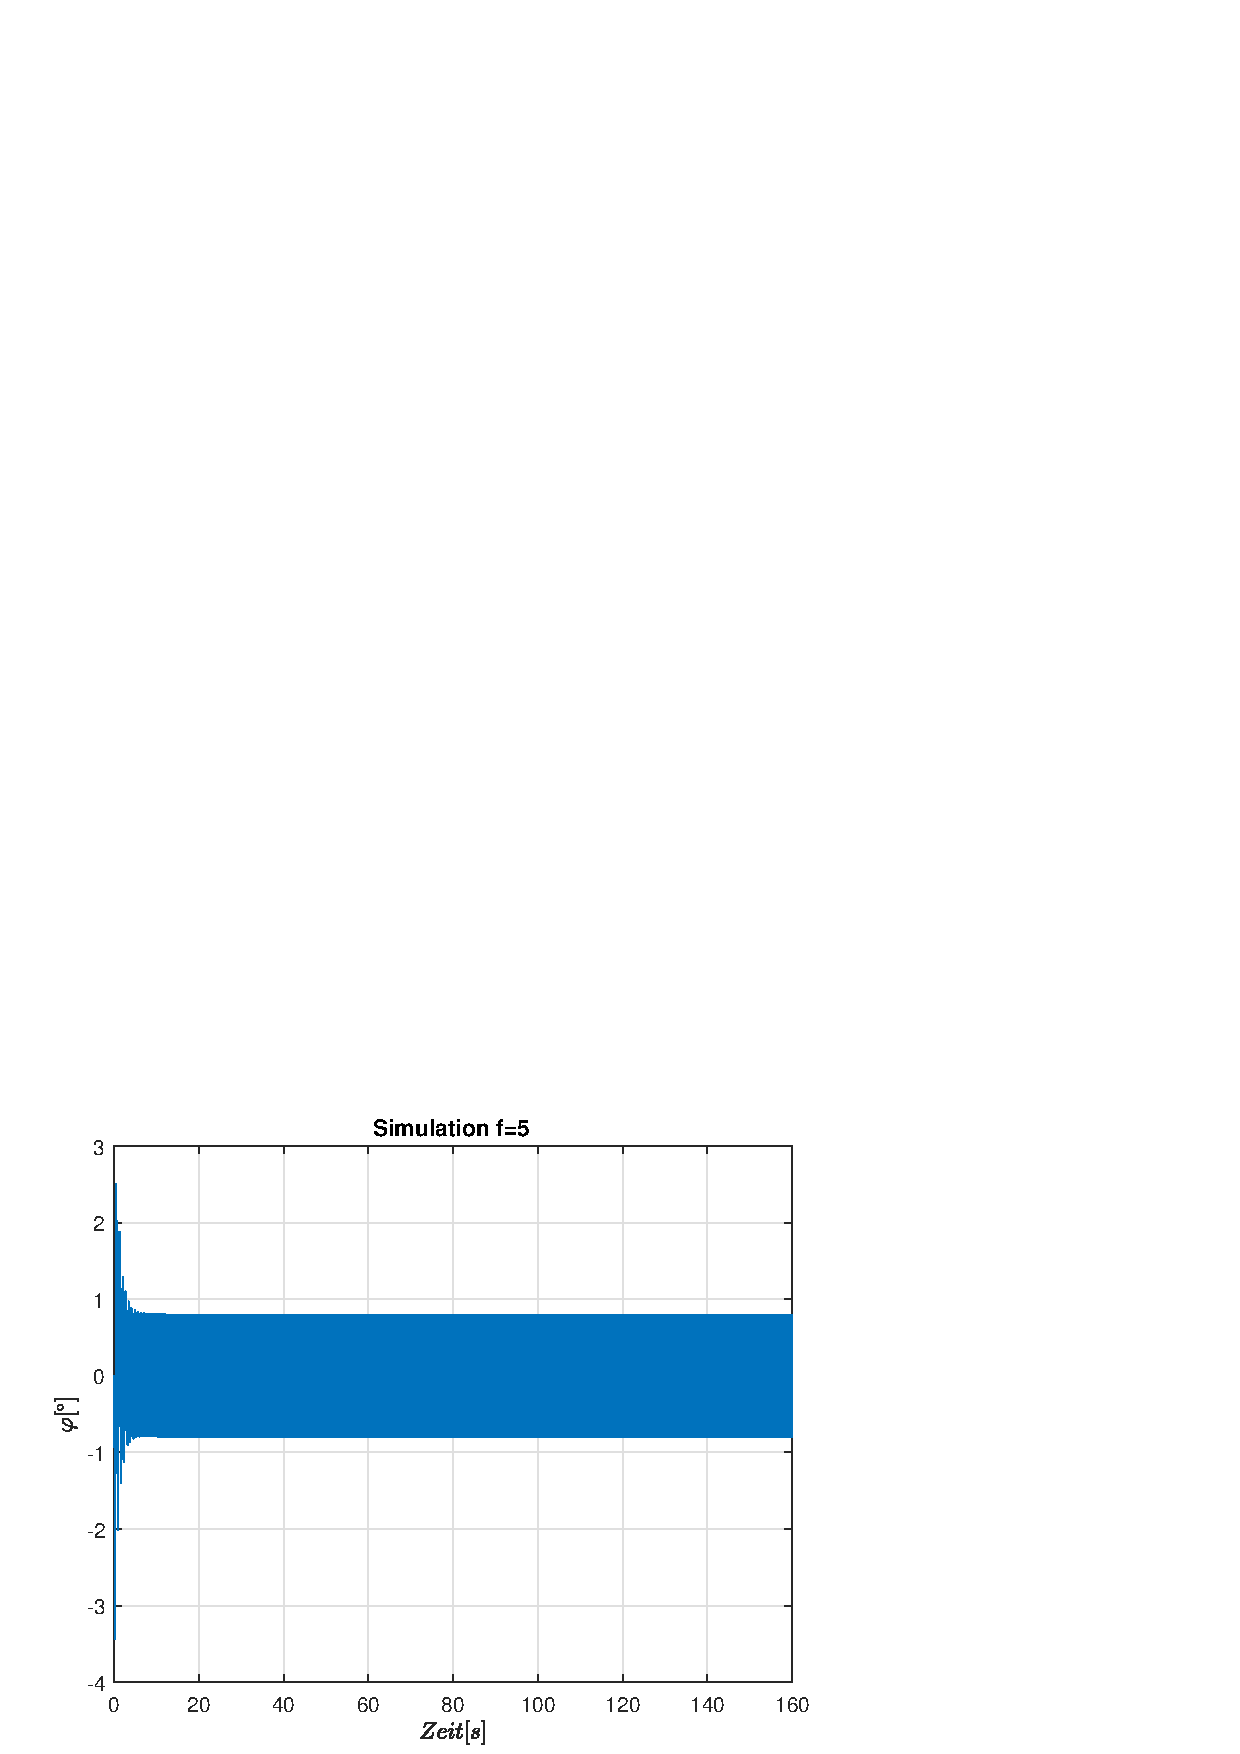
\includegraphics[width=0.5\linewidth]{img/sim_phi_sine_freq_5}
\end{figure}
\begin{figure}[!h]
\includegraphics[width=0.5\linewidth]{img/sim_phi_sine_freq_6}
\includegraphics[width=0.5\linewidth]{img/sim_phi_sine_freq_7}
\end{figure}
\begin{figure}[!h]
\includegraphics[width=0.5\linewidth]{img/sim_phi_sine_freq_8}
\includegraphics[width=0.5\linewidth]{img/sim_phi_sine_freq_9}
\end{figure}
\begin{figure}[!h]
\centering
\includegraphics[width=0.5\linewidth]{img/sim_phi_sine_freq_10}
\end{figure}

\newpage
\subsubsection{DFT-Spektren von $\varphi$ bei $T_M = sin(2\pi\cdot f \cdot t)$}
\begin{figure}[!h]
\includegraphics[width=0.5\linewidth]{img/sim_fft_sine_freq_0_5}
\includegraphics[width=0.5\linewidth]{img/sim_fft_sine_freq_1}
\end{figure}
\begin{figure}[!h]
\includegraphics[width=0.5\linewidth]{img/sim_fft_sine_freq_2}
\includegraphics[width=0.5\linewidth]{img/sim_fft_sine_freq_3}
\end{figure}
\begin{figure}[!h]
\includegraphics[width=0.5\linewidth]{img/sim_fft_sine_freq_4}
\includegraphics[width=0.5\linewidth]{img/sim_fft_sine_freq_5}
\end{figure}
\begin{figure}[!h]
\includegraphics[width=0.5\linewidth]{img/sim_fft_sine_freq_6}
\includegraphics[width=0.5\linewidth]{img/sim_fft_sine_freq_7}
\end{figure}
\begin{figure}[!h]
\includegraphics[width=0.5\linewidth]{img/sim_fft_sine_freq_8}
\includegraphics[width=0.5\linewidth]{img/sim_fft_sine_freq_9}
\end{figure}
\begin{figure}[!h]
\centering
\includegraphics[width=0.5\linewidth]{img/sim_fft_sine_freq_10}
\end{figure}


\newpage
\subsubsection{Autokorelleation von $\varphi$ bei $T_M = sin(2\pi\cdot f\cdot t)$}
\begin{figure}[!h]
\includegraphics[width=0.5\linewidth]{img/sim_rxx_sine_freq_0_5}
\includegraphics[width=0.5\linewidth]{img/sim_rxx_sine_freq_1}
\end{figure}
\begin{figure}[!h]
\includegraphics[width=0.5\linewidth]{img/sim_rxx_sine_freq_2}
\includegraphics[width=0.5\linewidth]{img/sim_rxx_sine_freq_3}
\end{figure}
\begin{figure}[!h]
\includegraphics[width=0.5\linewidth]{img/sim_rxx_sine_freq_4}
\includegraphics[width=0.5\linewidth]{img/sim_rxx_sine_freq_5}
\end{figure}
\begin{figure}[!h]
\includegraphics[width=0.5\linewidth]{img/sim_rxx_sine_freq_6}
\includegraphics[width=0.5\linewidth]{img/sim_rxx_sine_freq_7}
\end{figure}
\begin{figure}[!h]
\includegraphics[width=0.5\linewidth]{img/sim_rxx_sine_freq_8}
\includegraphics[width=0.5\linewidth]{img/sim_rxx_sine_freq_9}
\end{figure}
\begin{figure}[!h]
\centering
\includegraphics[width=0.5\linewidth]{img/sim_rxx_sine_freq_10}
\end{figure}

\newpage
\subsubsection{Leistungsdichtespektren von $\varphi$ bei $T_M = sin(2\pi\cdot f\cdot t)$}
\begin{figure}[!h]
\includegraphics[width=0.5\linewidth]{img/sim_lds_sine_freq_0_5}
\includegraphics[width=0.5\linewidth]{img/sim_lds_sine_freq_1}
\end{figure}
\begin{figure}[!h]
\includegraphics[width=0.5\linewidth]{img/sim_lds_sine_freq_2}
\includegraphics[width=0.5\linewidth]{img/sim_lds_sine_freq_3}
\end{figure}
\begin{figure}[!h]
\includegraphics[width=0.5\linewidth]{img/sim_lds_sine_freq_4}
\includegraphics[width=0.5\linewidth]{img/sim_lds_sine_freq_5}
\end{figure}
\begin{figure}[!h]
\includegraphics[width=0.5\linewidth]{img/sim_lds_sine_freq_6}
\includegraphics[width=0.5\linewidth]{img/sim_lds_sine_freq_7}
\end{figure}
\begin{figure}[!h]
\includegraphics[width=0.5\linewidth]{img/sim_lds_sine_freq_8}
\includegraphics[width=0.5\linewidth]{img/sim_lds_sine_freq_9}
\end{figure}
\begin{figure}[!h]
\centering
\includegraphics[width=0.5\linewidth]{img/sim_lds_sine_freq_10}
\end{figure}



\end{document}